\documentclass[fontsize=12pt,paper=letter,cleardoublepage=plain,twoside=false]{scrbook}

% adapted from https://github.com/jonhoo/thesis/

% for 1.5 line spacing
\usepackage{setspace}
\onehalfspacing
% single spacing for table of contents
\AfterTOCHead{\singlespacing}

% recompute page layout based on the above
\recalctypearea

% more colors (like RedOrange)
\usepackage[dvipsnames]{xcolor}

% qualitative colors
% subset of https://jfly.uni-koeln.de/color/
% that is also distinctive in grayscale
\definecolor{set1}{HTML}{0071b2} % blue
\definecolor{set2}{HTML}{e59c00} % orange
\definecolor{set3}{HTML}{009e73} % green
\definecolor{set4}{HTML}{efe440} % yellow

% so we can splice in PDFs
\usepackage{pdfpages}

% set up bibliography
\usepackage[square,comma,numbers,sort&compress]{natbib}

% enumerate* and itemize*
\usepackage[inline]{enumitem}

% for \begin{comment}
\usepackage{verbatim}

% for source-code listings
\usepackage[newfloat,draft=false]{minted}

% for formulas
\usepackage{mathtools}

% to split lists into multiple columns
\usepackage{multicol}

% for "on page NN" reference
\usepackage[nospace]{varioref}

% for \sfrac
\usepackage{xfrac}

% for \ifoptionfinal
\usepackage{ifdraft}

\usepackage[breaklinks, pdfborder={0 0 0}]{hyperref}
\usepackage[nameinlink]{cleveref}

% for \num, used in \loc macro
\usepackage[group-separator={,}]{siunitx}

% do not reset page numbers at \mainmatter
\let\mainmatterorig\mainmatter
\renewcommand\mainmatter
 {\edef\p{\arabic{page}}%
  \mainmatterorig
  % we need to compute the actual current page number. we know the page number
  % from _before_ we called \mainmatter. but what is it now? well, it is
  % certainly that +1. but we also need to account for the next chapter starting
  % on a "right" (odd) page. we do this by adding the page number modulo two.
  % TODO: double check before final version
  \setcounter{page}{\p+1+(\p-\p/2*2)}%
 }

% an environment for todos
\newenvironment{inprogress}
  {\vspace{.5em} \color{set2} \noindent \textbf{TODO}}
  {\vspace{.5em}}
\newcommand{\insertnote}[3]{\noindent\textcolor{#1}{\textbf{#2:} #3}}
\newcommand{\note}[1]{\insertnote{blue}{NOTE}{#1}}
\newcommand{\todo}[1]{\insertnote{red}{TODO}{#1}}

% a command to indicate current editing progress
\newcommand{\resume}{
  \begin{center}
    \color{set2}
    \hrule
    \vspace{1pt}
    \hrule
    \hrule
    \vspace{10pt}
    \textbf{This section is not yet complete.}
    \vspace{10pt}
    \hrule
    \hrule
    \vspace{1pt}
    \hrule
  \end{center}
}

\usepackage{relsize}
\renewcommand{\ttdefault}{pxtt}
\newcommand{\horizontalrule}{\rule{\textwidth}{0.5pt}}

%% semantic formatting
\newcommand{\code}[1]{\texttt{\detokenize{#1}}}
\newcommand{\cc}[1]{\mbox{\smaller[0.5]\texttt{\detokenize{#1}}}}
\newcommand{\scc}[1]{\mbox{\textsc{\detokenize{#1}}}}
\npthousandsep{,}
\newcommand{\loc}[1]{\numprint{#1}}

% \newidentmacro{foobar} creates \foobar that expands to foobar, with the right
% formatting to be an identifier.
\newcommand{\newidentmacro}[1]{\csdef{#1}{\mathtt{#1}}}
% \newdefmacro{foobar} is like \newidentmacro but it uses textlog to format the
% identifier
\newcommand{\newdefmacro}[1]{\csdef{#1}{\textlog{#1}}}

\newcommand{\tightenspace}{\vspace{-\baselineskip}}

%% Code

\newcommand{\load}[1]{\operatorname{Load}(#1)}
\newcommand{\store}[2]{\operatorname{Store}(#1, #2)}

%% notation

% https://tex.stackexchange.com/questions/4194/how-to-typeset-haskell-operator-and-friends
\newcommand\mdoubleplus{\ensuremath{\mathbin{+\mkern-10mu+}}}
\newcommand{\mapupd}[2]{[#1 \mapsto #2]}

%% iris.sty extensions for Perennial

\newcommand{\sep}{*}

% \newcommand{\wpc}[3]{\operatorname{wpc} \, #1 \, \{#2\} \, \{#3\}}
\NewDocumentCommand\wpc{O{} m O{} o m m}%
  {\textlog{\syntax{wpc}}^{#1}_{#3\IfValueT{#4}{,#4}}\spac#2\spac{\syntaxbraced{#5}}\spac{\syntaxbraced{#6}}}

\newcommand{\recoverwith}{\circlearrowleft}
\NewDocumentCommand\wpr{O{} m m O{} m m}%
  {\textlog{\syntax{wpr}}^{#1}_{#4}\spac#2 \recoverwith #3 \spac{\syntaxbraced{#5}}\spac{\syntaxbraced{#6}}}

\newcommand{\wpcw}{\textlog{wpc}\xspace}
\newcommand{\wprw}{\textlog{wpr}\xspace}
\newcommand{\wpw}{\textlog{wp}\xspace}

\newcommand{\notval}[1]{\neg \textlog{value(#1)}}
\newcommand{\cbmask}{\textlog{B}}

\NewDocumentCommand \hoareC {m m m m}{
  \curlybracket{#1}\spac #2 \spac \curlybracket{#3}\curlybracket{#4}%
}

\NewDocumentCommand \hoareCV {O{c} m m m m}{
  {\begin{aligned}[#1]
      &\curlybracket{#2} \\
      &\quad{#3} \\
      &\curlybracket{#4} \\
      &\curlybracket{#5}
    \end{aligned}}%
}

\newcommand{\postcrash}{\mathop{\blacklozenge}}
\newcommand*{\preborrow}{\textlog{preborrow}}
%\newcommand*{\cInv}[2]{{\boxedassert{#1 \mathop{|} #2}}^{\lightning}}
\newcommand*{\cInv}[2]{{\boxedassert{#1 \mathop{|} #2}}}
%\NewDocumentCommand \cfupd {O{} O{}} {\mathord{{}^\lightning\kern-1.15ex\vsGen[]{{\mid\kern-0.5ex\Rrightarrow\kern-0.25ex}}^{#1}_{#2}\kern0.2ex}}

\newcommand{\SKIP}{\mathit{noop}}
\renewcommand{\Ret}[1]{\text{\textbf{ret}}\,\, #1,\,}

%% more Perennial stuff

\newcommand{\lock}[1]{\textlog{acquire}(#1)}
\newcommand{\unlock}[1]{\textlog{release}(#1)}
\newcommand{\newlock}{\textlog{newlock}()}

\newcommand{\prelock}[1]{\textlog{preLock}(#1)}
\newcommand{\islock}[2]{\textlog{isLock}(#1, #2)}
\newcommand{\locked}[1]{\textlog{locked}(#1)}

%\newcommand{\precrashlock}[1]{\textlog{preCrashLock}(#1)}
\newcommand{\iscrashlockNoArgs}{\textlog{isCrashLock}}
\newcommand{\iscrashlock}[3]{\iscrashlockNoArgs(#1, #2, #3)}
\newcommand{\crashlockedNoArgs}{\textlog{crashLocked}}
\newcommand{\crashlocked}[3]{\crashlockedNoArgs(#1, #2, #3)}
\newcommand{\precrashlock}[1]{\textlog{preCrashLock}(#1)}

% Disk FFI
\newcommand{\diskwriteNoArgs}{\textlog{DiskWrite}}
\newcommand{\diskreadNoArgs}{\textlog{DiskRead}}
\newcommand{\diskwrite}[2]{\diskwriteNoArgs(#1, #2)}
\newcommand{\diskread}[1]{\diskreadNoArgs(#1)}
\newcommand{\dmapsto}{\mapsto_\textsf{d}}
\newcommand{\vals}{vs}
\newcommand{\block}{b}
\newcommand{\addr}{a}

\newcommand{\memory}{m}
\newcommand{\disk}{d}

% newly defined here (durable(P) := P |- post_crash(P))
\newcommand{\durable}{\textlog{durable}}

%%% GoJournal

% abbreviations
\newcommand{\fstar}{F${}^\star$\xspace}
\newcommand{\lowstar}{Low${}^\star$\xspace}
\newcommand{\lambdarust}{$\lambda_{\mathrm{Rust}}$\xspace}
\newcommand{\safe}{\mathrm{safe}}

% GoJournal total
\newcommand{\gotxnLOC}{\loc{1345}}
\newcommand{\gotxnLOP}{\loc{25797}}
%

%%% DaisyNFS

% soundness definitions
\newcommand{\refines}{\sqsubseteq}
\newcommand{\progeq}{\approx}

% ``type arg'', to write something like Goose<L>. I'm using angle brackets to
% match C++ and Rust.
\newcommand{\targ}[1]{\langle #1 \rangle}
\newcommand{\layer}{L}
% the type of operations O
\newcommand{\OP}{\mathcal{O}}
\newcommand{\crash}{\operatorname{crash}}
\newcommand{\gooselayervar}[1]{\ensuremath{\mathtt{Go}\targ{\mathit{#1}}}}
\newcommand{\gooselayer}[1]{\ensuremath{\mathtt{Go}\targ{\mathrm{#1}}}}
\newcommand{\compile}{C}
\newcommand{\impl}{I}
\newcommand{\init}{\operatorname{init}}

\newcommand{\server}{\texttt{s}}
\newcommand{\sdfy}{\ensuremath{\server_{\mathrm{dfy}}}}
\newcommand{\sdfyAlt}{\ensuremath{\tilde{\server}_{\mathrm{dfy}}}}
\newcommand{\stxn}{\sdfy}
\newcommand{\ssys}{\ensuremath{\server_{\mathrm{sys}}}}
\newcommand{\snfs}{\ensuremath{\server_{\mathrm{NFS}}}}
\newcommand{\infs}{\ensuremath{i_{\mathrm{NFS}}}}
\newcommand{\txncode}{\texttt{txn}}
\newcommand{\linked}[1]{\ensuremath{\mathrm{link}(#1, \txncode)}}
\newcommand{\linkedcode}{\linked{\sdfy}}
\newcommand{\Sys}{\mathit{Sys}}
% op as a variable
\newcommand{\opv}{\mathit{op}}

\newcommand{\seqrefinement}{\operatorname{seq\_refinement}}
\newcommand{\seqrefinementdfy}{\seqrefinement_{\mathrm{dfy}}}

\newcommand{\atomically}[1]{\ensuremath{\mathtt{atomically}\,\{\, #1 \,\}}}
\newcommand{\atomiccomp}{\mathtt{atomically}\circ}

%%% Goose

% spacing for application
\newcommand{\app}{\:}
\newcommand{\seq}{;\,}
\newcommand{\defeq}{\triangleq}
\newcommand{\lappend}{\mdoubleplus}

\newcommand{\goosedef}[1]{\mathsf{#1}}
\newcommand{\goosekw}[1]{\ensuremath{\goosedef{\textcolor{blue}{#1}}}}
\newcommand{\goosetrue}{\goosekw{true}}
\newcommand{\goosefalse}{\goosekw{false}}

% \gooseif{c}{e1}{e2} -> if c then e1 else e2
\newcommand{\gooseif}[3]{\goosekw{if} \app #1 \app%
  \goosekw{then} \app #2 \app \goosekw{else} \app #3}

% \gooselet{x}{e1}{e2} -> let x = e1 in e2
% the random extra {}'s around the = are so that LaTeX doesn't group anything
% with it (eg, let tmp = !x)
\newcommand{\gooselet}[3]{\goosekw{let} \app #1 {} = {} #2 \app \goosekw{in} \app #3}


% for handy reference
%
% paragraph without spacing:
% \setparsizes{0pt}{0pt}{0pt plus 1fil}

% in thesis: titlehead, subject, title, subtitle
\title{Verifying a concurrent, crash-safe file system}
\author{Tej Chajed}
\begin{document}

\frontmatter

% always arabic page numbering (default is roman in \frontmatter)
\pagenumbering{arabic}

\section*{Acknowledgments}
\begin{spacing}{1}
  \ifoptionfinal{\tej{write the acknowledgments}
}{Will be included in the final submission.}
\end{spacing}
\cleardoublepage

\section*{Prior Publication}
Parts of this thesis were previously published in a conference
paper~\cite{chajed:gojournal}.
\cleardoublepage

\tableofcontents

\mainmatter

\chapter{Introduction}%
\label{sec:introduction}
One crucial service in an operating system is its \emph{file system}, the
software that implements the abstraction of files and directories on top of a
disk, which simply stores a long sequence of bytes. File systems are important
because they are used by all applications to store data, and bugs in file
systems are especially costly because they can lead to data loss for any of
these applications. One approach to improve reliability is to use formal
verification, in which the file system is developed along with a proof that it
always follows a high-level specification of its intended behavior. This thesis
develops new techniques to address the key challenges in a file system of
reasoning about \emph{concurrency} and unexpected \emph{crashes} where the whole
computer reboots, a verified transaction system that handles these concerns, and
a file system that uses the transaction system. The final artifact is DaisyNFS,
a verified file system that comes with a proof of correctness and that achieves
good performance.

\section{Motivation}
\label{sec:intro:motivation}

A file system is an especially critical system for
three reasons. First, the file system is widely used --- essentially all applications have
data that is ultimately stored in a file system. Second, implementations are
concurrent and optimized, which increases the potential for bugs. Finally, bugs
are particularly costly since they can lead to permanent data loss for any
application running on top.

Two challenges make implementing a correct file system challenging: crashes and
concurrency. A file system is generally expected to keep application data safe
even if the system stops running at any time, say due to a power failure or
kernel panic. This thesis uses ``crash'' to refer to any of these circumstances
where the computer stops and is rebooted. After a reboot, the file system is
expected to preserve data from before the crash. The second big challenge is
concurrency in the implementation, which complicates approaches for improving
reliability, including both testing and verification.

Bugs are still discovered in widely used file systems like ext4 and btrfs,
despite a long history of developing, testing, and using these file systems. A
recent approach for fuzzing file systems~\cite{kim:hydra} found new crash-safety
issues in both ext4 and btrfs, despite not testing for concurrency issues. A
study conducted in 2013 looked at all patches for Linux file systems from
2005--2013~\cite{lu:fsstudy}, finding hundreds of these patches were to fix bugs
(for example, 450 for ext4 and 358 for btrfs). About 60\% of these bugs lead to
data loss or crash the kernel (and as the study points out, these are much more
serious consequences than most bugs in application software). File systems have
a lot of internal concurrency for performance reasons, which both leads to bugs
and makes testing and fuzzing more challenging.

The approach in this thesis to make a reliable file system is to use formal
verification. In this approach, we write the code, then a specification of the
intended behavior of the code, and finally a mathematical proof that shows the
code always meets the specification. For confidence in the proof itself, the
proof is carried out in a computer and a piece of software called a proof
assistant checks that the proof is valid. The nature of formal verification
forces the proof engineer to systematically cover every corner case in the code.
As a result, they can completely rule out whole classes of bugs, including
low-level bugs like memory safety but also logic errors like returning the wrong
data. Verification does not guarantee that a system is bug-free, because the
specification must be correct and the assumptions in the proof must hold in
practice, but it does help since the specification is smaller than the
implementation, and it isolates debugging to identifying where the specification
is wrong or an assumption was violated.

While the idea of formal verification is not new, there was essentially no
support for reasoning about the combination of crashes and concurrency when this
thesis work started (in 2015). Thus this thesis develops new techniques to
reason about the combination in the first place. We apply these techniques to
DaisyNFS, a verified implementation of the Network File System (NFS) protocol, a
standard file-system interface.

The key to verifying a system with the complexity of DaisyNFS is a design
that splits the file system into two main parts: a transaction system called
GoTxn that makes it easy to get atomicity over the disk, and then the rest of
the file system implemented using a transaction per operation. GoTxn must face
the key challenges of crash safety and concurrency, but it handles them in such
a way that the code on top is verified using comparatively much simpler
sequential reasoning. The file-system code then focuses on implementing features
like the details of the NFS semantics, large files, and efficient data
structures.

\section{State of the art}
\label{sec:intro:related}

Production file systems are generally validated by testing. While testing is
indispensable for development, the nature of a file system makes it difficult to
catch all bugs with only testing. The fundamental difficulty is a high degree of
non-determinism from two sources: crashes in the middle of execution, and
concurrency in the implementation that is needed for good performance.

The importance of file-system correctness has been recognized by the academic
community, thus there are many approaches for increasing confidence with
improved testing. One line of work has explored systematically testing crashes
at intermediate points~\cite{mohan:crashmonkey,pillai:appcrash,yang:explode}. Another line of
work has focused on fuzz testing as a way to induce crash-safety
bugs~\cite{xu:janus,kim:hydra}. These approaches have been successful for
finding bugs, including crash-safety bugs, but they only test sequential
executions, missing bugs due to concurrently issued operations or from crashes
that interrupt multiple operations. Furthermore, unlike formal verification, testing cannot
cover all executions of a program, even without crashes and concurrency,
potentially missing bugs.

The research community has also recognized the value of formal verification for
reasoning about a file-system implementation. The closest related work is
Flashix~\cite{bodenmuller:concurrent-flashix}, a verified, concurrent file
system that runs on flash devices. The techniques
developed to verify Flashix are specialized to its particular file-system
design, especially its write-back cache. Its concurrency is primarily between
regular operations and garbage collection, and read-only concurrency. This
thesis develops a general logic for reasoning about crashes and concurrency and
applies this logic to verify a system with write-write concurrency.

There are other verified file systems, especially the sequential file systems
FSCQ~\cite{chen:fscq} and Yggdrasil~\cite{sigurbjarnarson:yggdrasil} and an
concurrent but in-memory file system AtomFS~\cite{zou:atomfs}. These systems use
verification techniques that do not support both crashes and concurrency, and they
cannot be extended them in a straightforward way to support the other form of reasoning.

\section{Approach}
\label{sec:intro:approach}

What does it mean to give a machine checked, formal proof of a system? At a high
level, program proofs always have three components: an implementation, a
specification, and a proof. When doing machine-checked proofs, all three are
physically represented as code in a verification system. The verification system
checks the proof against the implementation and specification, ensuring that the
proof is complete.

This thesis integrates interactive, foundational proofs using custom
infrastructure (in Coq) as well as automated verification using a
verification-aware programming language (Dafny). These are both machine-checked,
formal proofs, but the interaction models of the two systems are different
enough that this section describes them separately.

In Coq, the core feature is proofs based on dependent type theory, which is
expressive enough to represent essentially any math. A first step when using Coq
is to connect the code to the reasoning in the proof assistant. The particular
approach in this thesis translates executable code to a model in Coq,
implemented by a tool called Goose. The model
and its semantics encodes the
assumptions the proof makes about how the program behaves. The semantics is typically structured as a transition
system, where an execution is a sequence of states the program goes through
along with some notion of observable behavior, like external I/O or return
values. \tej{maybe add a figure of an execution trace}

Once we have a program in Coq, we can reason about it. The goal of
verification is to prove that the program meets its specification, and
where the specification describes the allowed behaviors of the program. The
specifications in this work forbid universally incorrect behavior, like reading an
out-of-bounds address in an array, but more precisely specify what the program
is supposed to do, for example how it responds to user requests.

A common structure to tame the complexity of reasoning about a program is to use
a \emph{program logic}. In principle it might be possible to prove a theorem
about all the behaviors of a program directly, but such a proof would too
complex to be feasible. The program logic organizes the proof with a structured
way of expressing and proving statements about the program, such as breaking the
proof down into theorems about individual functions. The proof in a program
logic will often mirror the structure of the code, since each function has its
own specification and groups of related functions have related specs.

Program logics for concurrency are still an active area of research; only
recently have they reached the maturity to give completely mechanized proofs of
moderate-sized programs. There are few logics that also can reason about crash
safety. Our approach in this thesis is to build a new program logic called Perennial with all the
concurrency-reasoning features of a modern program logic, plus new features for
reasoning about crashes. What makes this feasible is Iris, a modular framework
for concurrency. Iris includes a concurrent program logic which we are able to
extend with crash-safety reasoning while preserving the concurrency reasoning
features, without reimplementing them from scratch.

Using our new program logic, we verified GoTxn, a concurrent transaction system.
The transaction system's correctness theorem says that any program that uses
transactions really has transactional behavior: its execution is equivalent to a
version of the program where the transactions run atomically. The complete
specification includes some important details in order to formalize the
intuition behind atomicity.

Next, because transactions appear to run sequentially, and write to disk all at
once, it is no longer necessary to use a sophisticated program logic like
Perennial to reason about the body of each transaction. Instead, we switch to
using Dafny, a verification-oriented programming language that only supports
sequential code but as a result is highly productive for this use case. The file
system is written and verified in Dafny, then compiled to Go and linked with
GoTxn.

Dafny verification works quite differently from Coq. Dafny is a programming
language with verification features; contrast this with Coq, which supports
general math that can \emph{model} programs. A Dafny method can be annotated
with a specification. The Dafny checker converts a method and its specification
to a logical formula (called a verification condition), which is true if and only if the specification holds for
the method. It then queries a \emph{solver} (Z3, in the case of Dafny) to determine if the formula is true.
Contrast all of this with Coq, where the user manually develops the program
logic and connects the rules of this logic. Checking a program against its specification in Dafny cannot be perfectly
automated because it is impossible to answer whether a general logical formula
is true or not, but the user can insert annotations to help out the solver, and
generally fewer annotations are needed than lines of proof for Coq. The main
downside to this approach is that it fixes a sequential programming language, so
unlike in Coq, it isn't possible to reason about concurrency and crashes.

\Cref{fig:overview} depicts how all of the components of DaisyNFS and its proof
fit together. The left-hand side depicts the implementation, split between GoTxn
and the file-system implemented in Dafny. The Dafny code is compiled to Go and
then the two parts are linked together into one \cc{daisy-nfsd} binary in the
usual Go build process. GoTxn is translated to a model using a tool called
Goose. The right-hand side of the figure depicts all aspects related to the
proof, which is written using the Perennial program logic. All of this happens
in the Coq proof assistant, which checks that the proofs are valid. Meanwhile
the DaisyNFS file-system code is verified in Dafny, which integrates
implementing, specifying, and verifying code. This proof is checked by the Dafny
verifier. Finally, the proof of GoTxn is written in such a way that it can be
composed with the proof of DaisyNFS for a theorem about the whole
\cc{daisy-nfsd} binary. This is a conceptual composition, not one in either
Dafny or Coq.

\begin{figure}[ht]
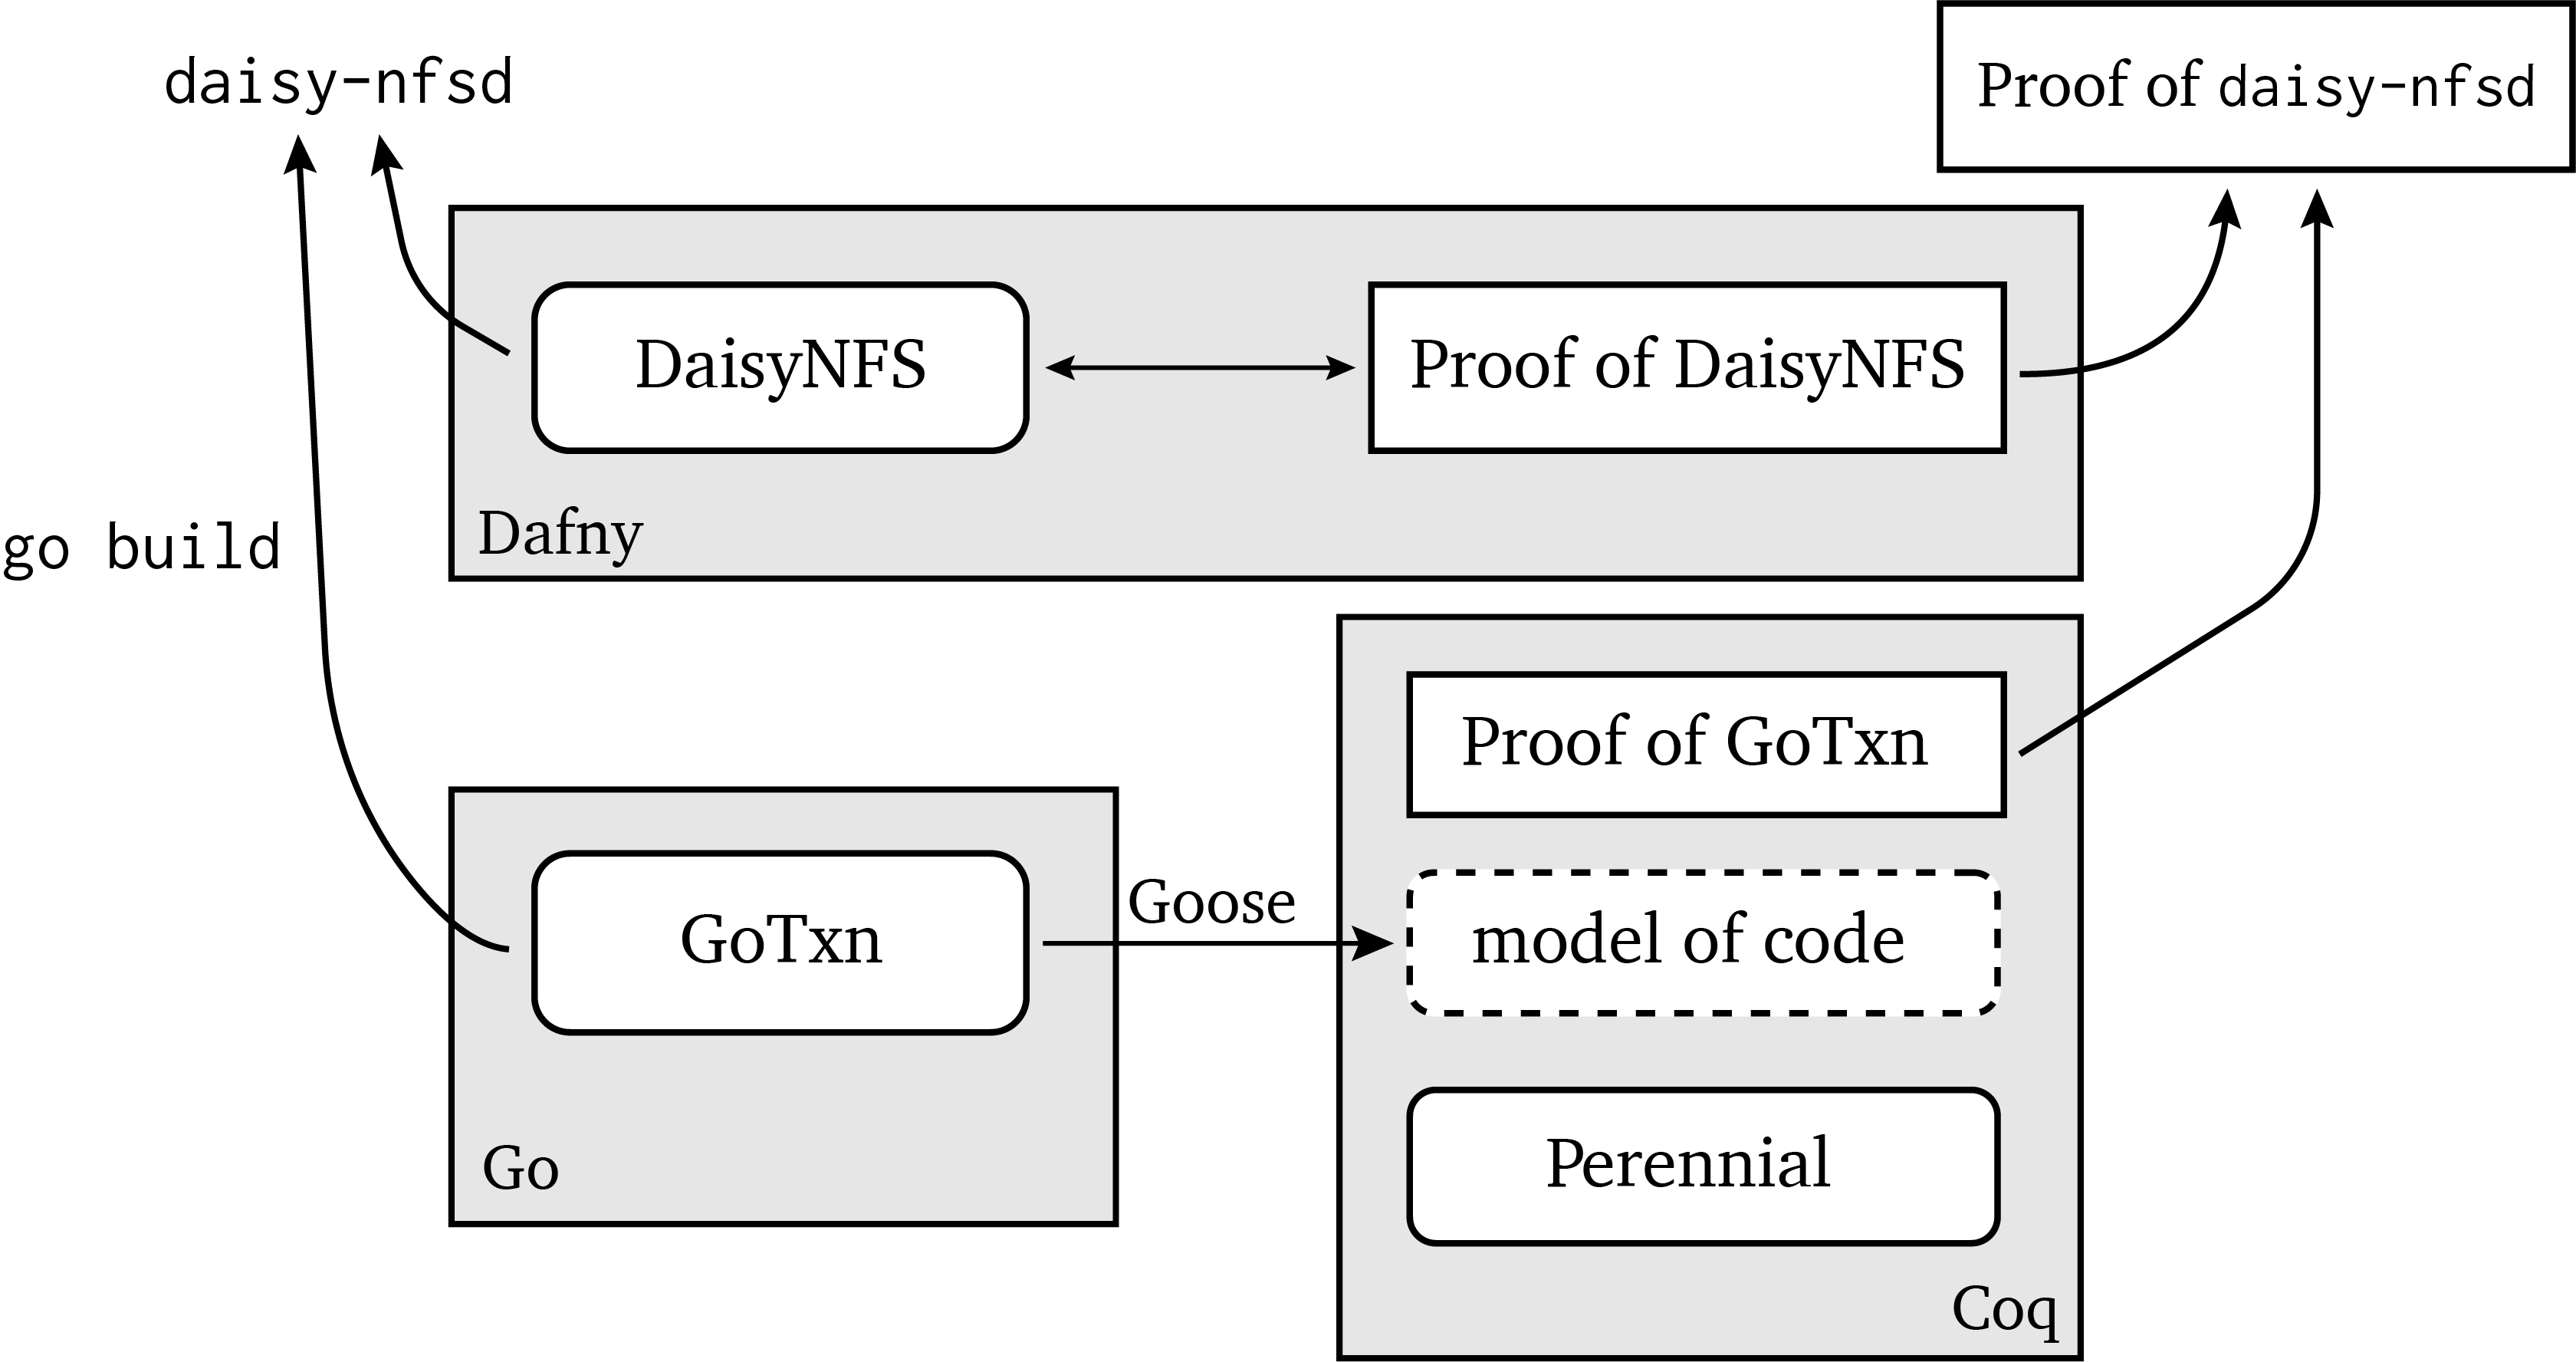
\includegraphics{fig/overview.png}
\caption{Overview of how GoTxn, DaisyNFS, and the proofs fit together.}
\label{fig:overview}
\end{figure}

One of the contributions of this thesis is that the file-system design isolates
concurrency and crash safety into the transaction system. This structure leaves
the rest of the implementation only to \emph{sequentially} implement the
file-system logic and data structures. Because this is sequential, crash-free
execution, we use Dafny to implement and verify each operation, then run this
code wrapped in a transaction. Intuitively what the file-system proof shows is
that it correctly implements the NFS protocol.

In order to connect the file system's sequential proofs to its concurrent
execution, we prove a general theorem about the transaction system's
implementation. The starting point is the idea of a \emph{simulation} proof,
which shows that a system like the file-system transactions correctly implement an
abstract specification like the NFS protocol. The GoTxn
\emph{simulation-transfer theorem} shows that for any system implemented using
transactions with a sequential simulation proof, the concurrent system running
with GoTxn concurrently simulates its abstract specification where each
operation is atomic. Intuitively this theorem holds because every concurrent
execution of the GoTxn transactions appears to be atomic, and then the
sequential simulation proof shows those atomic transactions implement the
abstract specification. However, the GoTxn theorem formalizes precisely what
conditions are required for the simulation transfer, including restrictions on
the transactions and exactly what crash safety guarantees are achieved.

\section{What is the value of verifying a file system?}

The reader might wonder what the value of this kind of large verification effort
is.

\paragraph{Cost versus benefit.} There are many less formal ways to make
software more reliable, including testing, fuzzing, and code auditing. Formal
verification also has a spectrum; we could potentially apply property-based
testing, model checking, or symbolic execution to parts of the code. Rather than
verifying the implementation, we could instead attempt to model and specify key
parts of the algorithms or system design, then verify those. What is the
additional value of fully machine-checked proofs, all the way down to the code?

Verification in the real world needs to have benefits that outweigh the costs.
The benefit of reliability for file systems is hopefully clear, from the
exposition above. I see this work as lowering the cost of verifying crash-safe
and concurrent systems: formerly, there simply didn't exist techniques for this
kind of proof, and now it is possible (and at least the cost is bounded by a PhD
thesis and not something much larger). Building on these foundations, I hope the
costs come down to make verification an appealing alternative to verification
for the next generation of storage systems.

The real ideal for verification is not just it is worth paying the costs but
that verification enables something that would otherwise not be doable. With
file systems I believe this is possible, since verification might enable a new
file system with more daring optimizations to gain confidence faster than would
otherwise be possible. There aren't that many widely-used file systems --- most
people use one of ext4, btrfs, or XFS on Linux, NTFS on Windows, and APFS on
macOS --- and new file systems are generally adopted very slowly. APFS was
surprising for having only a 3-year development period before Apply widely
deployed it, and this was probably only possible because of Apple's tight
vertical integration. Ext4 is the other ``new'' file system, introduced in 2008
(by extending ext3, which was first released in 2001).

% ext4: 2008
% ext3: 2001
% XFS: 1994 (first released on IRIX OS for SGI)
% NTFS: 1993
% APFS: 2017

\paragraph{Verification guides debugging.} With a verified system, bugs are
still inevitable since there is unverified code surrounding the verified code,
the assumptions of the proof can be violated, and the specification can be
wrong. However, an advantage of formal verification, particularly fully
machine-checked proofs, is that when bugs are discovered it's safe to start
debugging with all the code outside the verification as well as looking at the
specification.

\resume

\section{Contributions}
\label{sec:intro:contributions}

This thesis makes the following contributions that enable its overall goal of a
verified, concurrent file system:

\begin{itemize}
  \item \textbf{Perennial} is a program logic for crash safety
        and concurrency using specifications based on crash weakest
        preconditions. These include crash conditions combined with concurrency
        and reasoning principles for moving ownership to a recovery procedure
        following a crash. \textbf{Logically atomic crash specifications} are a
        pattern using Perennial's crash weakest preconditions for specifying
        libraries that have both concurrent behavior and involve persistent
        state. These are implemented using Perennial and used in the GoTxn
        proof.
  \item GoTxn has a new \textbf{lifting-based specification} for its journaling
        layer to reason about concurrent transactions separately, which is
        challenging since the logical disk can change in the middle of a transaction. Its proof uses a novel
        \textbf{history-based abstract state} for the write-ahead log. This model allowed us to carry
        out a modular proof where the write-ahead logging library hides most of
        its internal complexity, simplifying reasoning about the rest of the GoTxn
        code that uses it. Finally, GoTxn exports a \textbf{program refinement}
        specification that captures how transactions appear to run atomically.
  \item DaisyNFS uses a \textbf{simulation-transfer theorem}, proven on top of
        GoTxn's program refinement specification, which shows that sequential
        reasoning for each transaction in a system implies correctness for the
        whole system when run on top of GoTxn. This justifies using Dafny, a
        sequential verification language, to verify the DaisyNFS implementation.
        The specification for DaisyNFS uses a mathematical formulation of RFC
        1813, the document that (in prose) specifies what a NFSv3 server should
        do.
  \item \textbf{Goose} connects efficient code implemented in Go to a model of
        that code in Perennial. A general contribution here is a design for
        systems verification that enables efficient code and convenient
        reasoning. Goose includes reasoning principles for the models that it
        outputs, to support verifying the translated code.
\end{itemize}

The ideas in Perennial and Goose are applied to GoTxn, but they could be used
for reasoning about other concurrent storage systems. Similarly,
this thesis applied GoTxn to a verified file system, but it could also be used
as the basis for other verified storage systems, like a persistent key-value
store.

\tej{describe limitations at a high level}

\section{Reading guide for the thesis}
\label{sec:intro:reading-guide}

This section briefly outlines the chapters of the thesis, the dependencies
between chapters, and the intended audience. Broadly the thesis is intended for
a systems audience, except for the verification foundations. The support for
concurrency makes all of the formal underpinnings in the thesis more technical
than foundations for sequential systems verification.

\Cref{ch:related} covers related work across Perennial, GoTxn, and DaisyNFS, for
a broad computer-science audience. To keep the Goose chapter self-contained, its
related work is described in the relevant chapter.

\Cref{ch:perennial} is an overview of Perennial. This chapter is oriented
towards a reader interested in the general verification concepts and not
necessarily the systems side. At this level of abstraction Perennial is
independent of both the GoTxn proof and even Goose for verifying Go code. Some
experience with program logics is helpful for understanding the presentation.

\Cref{ch:crash-logatom} describes a style of logically atomic specifications
that capture both concurrency and crash atomicity using Perennial. It uses an
extended example from the GoTxn proof and explains its formal underpinnings at a
high level. This is the most technically involved chapter.

\Cref{ch:txn} describes the design and proof of GoTxn. An important part of GoTxn is its
specification, which captures how transactions are atomic. This chapter does not
require the full Perennial or logical atomicity chapters.

\Cref{ch:daisy-nfs} describes the design and proof of DaisyNFS.\@ This chapter
explains the proof approach that justifies using Dafny to verify DaisyNFS even
though Dafny is a sequential verification tool and DaisyNFS is a concurrent
system.

\Cref{ch:goose} is about Goose and talks about verifying Go code generally, with
nothing specific to GoTxn or even storage systems. This is the first detailed
description of Goose, so this chapter is written to be readable without any of
the other chapters.

\Cref{ch:impl} is a short chapter covering some implementation details in
DaisyNFS, covering both GoTxn and the file-system code.

\Cref{ch:eval} evaluates the whole file system along a few dimensions,
especially performance but also aspects of the proof.


\chapter{Related Work}%
\label{sec:related}
While verifying programs is an old idea, going back at least to Floyd and
Hoare's work in the late 1960s~\cite{floyd:meanings,hoare:logic}, prior to this
thesis (in 2015) there was almost no work on reasoning about a program's
execution in the presence of a crash, let alone the combination of concurrency
and crashes. The full pipeline of systems verification is also quite new:
connecting the formal reasoning to executable programs, writing machine-checked proofs, and scaling up the techniques to
systems with sizable implementations.

The Perennial framework for reasoning about crashes and concurrency draws on two
lines of research: sequential crash safety verification and concurrency
verification, described in
\cref{sec:rel:crashes,sec:rel:concurrency,sec:rel:crashes-concurrency}. DaisyNFS
draws from two other lines of prior work, on verified transactions and file
systems, described in \cref{sec:rel:verified-fs,sec:rel:verified-txn}.

The most closely related work is Flashix, another verified concurrent and
crash-safe file system. \Cref{sec:rel:flashix} compares the two systems'
contributions and results. Finally, \cref{sec:rel:txn} discusses some related work
on using transactions as part of a file system.


\section{Foundations for verifying sequential crash safety}
\label{sec:rel:crashes}

There are a variety of foundational tools for reasoning about crash safety,
largely for sequential systems.

FSCQ~\cite{chen:fscq,chen:dfscq,hchen-phd} is a sequential file
system verified with Crash Hoare Logic (CHL). CHL's basic specifications have
the form $\hoareC{P}{e}{Q}{Q_{c}}$, extending the Hoare triple $\hoare{P}{e}{Q}$
with a \emph{crash condition} $Q_{c}$ that holds at all intermediate points in the
function's execution. Crash conditions handle a core difficulty of crashes,
namely that they stop the system at some intermediate step. There are two
remaining challenges: a crash wipes in-memory state, and the system might crash again
while recovering after a crash. CHL connects the system's crash conditions to a
specification for recovery to handle these two issues. A crash predicate
transformation captures what can be assumed when recovery starts, and for
crashes during recovery CHL requires that recovery be \emph{idempotent} in the
sense that its crash condition implies its own precondition. CHL was used to
specify and verify FSCQ~\cite{chen:fscq} and a more performant successor
DFSCQ~\cite{chen:dfscq}.

Yggdrasil~\cite{sigurbjarnarson:yggdrasil} takes a different approach to crash
safety. The basic definition is \emph{crash refinement}, which says that a
system implements an interface correctly, including a specification for what a
crash followed by recovery is allowed to do. Note that unlike CHL this
specification is about a collection of methods implementing an abstract,
specification transition system, not about individual methods. Yggdrasil uses
crash refinement to specify and verify a file system comparable to the file
system in xv6, a teaching operating system. The implementation uses Z3 to check
crash refinement, which the authors show is able to handle a system of this
complexity by breaking down the implementation into small enough layers.

Argosy~\cite{chajed:argosy}, which I led the development of but is not part of
this thesis, combines aspects of FSCQ and Yggdrasil. The key new idea is to
develop the metatheory for \emph{recovery refinement} that shows how systems
compose when both have recovery procedures --- what is non-trivial to handle is
that a crash in the composed recovery procedure requires starting over from the
beginning. Recovery refinement can be viewed as an extension of crash refinement
with verified metatheory for recovery, largely left implicit in the Yggdrasil
paper. Argosy also shows how to encode the conditions of recovery refinement
using CHL so that a single layer is verified using the CHL program logic.

VeriBetrKV~\cite{hance:veribetrkv} takes yet another approach to reasoning about
crashes, this time friendly to encoding in Dafny, a sequential verification
system with integrated support for programming and verification. The main idea
related to crash safety is to adopt the style from
IronFleet~\cite{hawblitzel:ironfleet} and think of a storage system as a
distributed system made up of the CPU and the storage device. The extension
needed for crash reasoning is to add a crash transition to the storage device
that non-deterministically wipes any buffered but unacknowledged writes, and
then to show that when this happens it corresponds to an appropriate
application-level transition modeling crashes (similar to the crash refinement
definition from Yggdrasil and recovery refinement in Argosy, although this is
associated with a code transition rather than a dedicated recovery procedure).
VeriBetrKV is used to verify a persistent key-value store based on
B\textsuperscript{$\epsilon$} trees, a data structure that also underlies
BetrFS~\cite{jannen:betrfs}.

Perennial has crash conditions that look similar to CHL's crash conditions,
albeit as part of a concurrent program logic rather than a sequential one. We do
carry out a refinement proof in the style of Argosy, which is similar to the
specification style in VeriBetrKV and Yggdrasil, but because it is connected to
concurrent reasoning the proof techniques are more sophisticated.

\section{Foundations for verifying concurrent programs}
\label{sec:rel:concurrency}

There are a number of approaches proposed to verifying concurrent programs, and
Iris in particular is the basis for Perennial. It
would be hard to do justice to the historical development of concurrency
reasoning. Looking at approaches that are actively used in research and
connected to executable implementation, two broad strategies are commonly used:
developing concurrent \emph{program logics}, and using \emph{refinement}-based
techniques.

Many refinement-based techniques are based on the idea of \emph{reduction},
which appeared originally in Lipton's theory of ``movers''~\cite{lipton:movers}.
The idea behind reduction is to reason about a program through program
transformations that show the program is equivalent to a simpler program. These
techniques can reason about concurrency by showing that a concurrent program is
equivalent to a program with sequential or atomic regions. These ideas have been
used as part of the CIVL verifier~\cite{hawblitzel:civl,kragl:civl-layers} and
Armada~\cite{lorch:armada}; my own prior work on CSPEC~\cite{chajed:cspec} was
also based on movers, before starting Perennial. Reduction-based techniques
generally reason about a program through a series of transformations, each
making the program slightly simpler, keeping the proof of each transformation's
correctness more manageable.

One large verified system, CertiKOS, is based on a custom verification
infrastructure called Certified Concurrent Abstraction
Layers~\cite{gu:certikos-ccal} which based on refinement but not reduction. This
work is notable for verifying a system (a simple operating system) not just at
an abstract protocol level but all the way down to concurrent code. The proof
composes with the CompCert compiler correctness theorem to carry the guarantees
down to the assembly code of the operating system.

Program logics are an alternative approach based on giving specifications to
each function in the program, within a logic that has useful rules for proving
and composing specifications. Hoare logic is a classic program
logic for sequential programs that based on pre- and post-conditions.
Concurrency makes it harder to construct a logic that can usefully reason about
many concurrency patterns (completeness) while also giving specifications that
hold in the presence of concurrent threads (soundness). One productive line of
work has been based on concurrent separation logic (CSL)~\cite{brookes:csl}.

The Verified Software Toolchain is notable for connecting a CSL-based logic
(VST-Floyd) down to proofs of C code, including a connection to CompCert to
carry these guarantees down to assembly~\cite{cao:vst-floyd}. It has been used
for a number of sequential verified C programs and recently to some shared
memory C libraries.

Microsoft VCC~\cite{cohen:vcc,cohen:vcc-local} is another verification system
that is based on annotating C code with pre- and post-conditions and so-called
two-state invariants that are similar to rely-guarantee
reasoning~\cite{jones:rg,feng:lrg}. VCC is typically used to encode a form
of concurrent refinement reasoning while also using specifications similar to
that of a program logic. The system was used to verify a portion of Hyper-V. The
system is implemented as a verification-condition generator; unlike the program
logics described in this section, VCC has no soundness argument (even on paper)
to specify what its specifications mean and argue that it enforces the right
conditions for that meaning to hold.

Perennial builds directly on Iris~\cite{jung:iris-jfp}. Iris is a general
framework for concurrency, featuring a base logic with key features for
concurrency (step indexing and separation-logic resources, including
\emph{higher-order} resources used to define invariants for example) and a
program logic built on the base logic. This decomposition was valuable for
Perennial because we made two core changes to Iris: first, the program logic
itself is extended with crash safety reasoning, and second, the framework is
applied to our GooseLang models of Go code. In both cases the generality of Iris
was valuable, as the framework is not tied to reasoning about a particular
programming language or even to its usual program logic. Prior to this work,
Iris had not typically been used for reasoning about executable code (though
projects like RefinedC~\cite{sammler:refinedc} and our own work on Goose are
changing that).

\section{Reasoning about crashes and concurrency}
\label{sec:rel:crashes-concurrency}

Program logics other than Perennial have been developed for formal reasoning
about concurrent, crash-safe systems. Fault-Tolerant Concurrent Separation Logic
(FTCSL)~\cite{ntzik:faults} extends the Views~\cite{dinsdale:views} concurrency
logic to incorporate crash-safety. POG~\cite{raad:pog} is a program logic for
reasoning about the interaction of x86-TSO weak-memory consistency and
non-volatile memory. Both of these logics are only defined on paper, and do not
support mechanized proof. Perennial goes beyond their reasoning principles: it
includes ownership reasoning and its interaction with crashes, and a style of
logically atomic crash specifications for modularly specifying libraries and
composing their proofs. FTCSL and POG have no mechanism of modular proofs of
layers, which we found essential to scale verification to a file system.

In the case of x86-TSO with persistence, POG required a line of research to
define the semantics at the
ISA level, validating this semantics against the hardware and in conversations
with Intel engineers~\cite{raad:px86,raad:px86-extended}. A similar semantics effort defines the
semantics of ext4 under crashes, but without an accompanying program
logic~\cite{kokologiannakis:persevere}. It would be an interesting direction for
future work to combine the persistency semantics of x86 with Perennial, to
verify libraries that use non-volatile memory.

\section{Verified transaction systems}
\label{sec:rel:verified-txn}

As far as we know, GoTxn is the first transaction system that makes data durable
and has a verified implementation. There is much related work on verifying
aspects of transaction systems with and without durability, and on unverified
transaction systems.

\citet{ChkliaevHS99} verify serializability of two-phase locking and other
transaction concurrency control mechanisms in the PVS theorem prover. Their
proof formalizes two-phase locking as an abstract protocol consisting of
sequences of read, write, and locking operations, as opposed to a concrete
implementation as in GoTxn. \citet{pollak-2PL} uses a variant of the
CAP separation logic~\citep{dinsdale:cap} to give a pen-and-paper
proof of serializability for an abstract, protocol-level description of
two-phase locking, connecting the protocol to atomic reasoning about
transactions.

\citet{mohsen:stm} developed a framework for verifying software transactional memory algorithms, modeled
as I/O automata. They applied their framework to sophisticated STM algorithms, such as
NOrec algorithm~\cite{dalessandro:norec}. The STM algorithms considered do not
handle persistence, so the framework does not address crash-safety reasoning.

A specification called the Push/Pull model of
transactions~\cite{koskinen:pushpull} is similar to the \emph{lifting} technique
in the journal system's specification~(\cref{sec:txn:lifting}) --- the core
problem addressed is that a journal operation atomically modifies a small number
of objects, but other objects can change between the start of the operation and when
it commits. The Push/Pull model also discusses reasoning on top of the
specification, using Lipton's reduction~\cite{lipton:movers} rather than
separation-logic ownership to handle concurrency. However that work is about
on-paper specifications and proofs, while we also prove an implementation meets
our specification and proved DaisyNFS on top.

DFSCQ~\cite{chen:dfscq} verifies a high-performance file system built on top of
a logging system with asynchronous disks and log-bypass writes, which are
challenging optimizations that GoTxn does not support. ARIES is a database
write-ahead logging protocol that was verified (with a pen-and-paper proof) in
FTCSL~\cite{ntzik:faults}; it is more sophisticated than GoTxn's write-ahead log
in that it can both undo and redo operations.

An important but unverified journaling system is jbd2, the ``journaling block
device'' that underpins ext3 and ext4 in Linux. The design of jbd2 is broadly
similar to that of GoTxn's journaling layer; GoTxn goes one step further and
also has automatic locking for transactions. One difference in the interfaces of
GoTxn and jbd2 is that in jbd2, transactions can reserve space ahead of time.
This has the benefit that a transaction can start writing to the journal on disk
while it is being prepared, potentially improving performance, but it also means
that a concurrent transaction must wait for all previously started transactions
to finish before becoming persistent, since a journaled operation can only be
logically completed when all prior operations are finished. This is a reasonable
tradeoff for a file system since transactions are generally short-lived, but it
sacrifices a bit of tail latency when an operation must be persisted, for
example when an application issues an \cc{fsync()}.

\section{Verified file systems}
\label{sec:rel:verified-fs}

The Dafny side of DaisyNFS is a new implementation but its design and aspects of
the proof strategy were inspired by other verified file systems like
DFSCQ~\cite{chen:dfscq} (especially its indirect block implementation described
in Alex Konradi's master's thesis~\cite{akonradi-meng}) and
Yggdrasil~\cite{sigurbjarnarson:yggdrasil}.

AtomFS~\cite{zou:atomfs} is a verified, concurrent file system, but its
implementation does not store data durably. The proof structure is quite
different from DaisyNFS in that all of the concurrency reasoning is part of the
file-system operations and there is no interaction between persistence and
concurrency. AtomFS is verified using a relational logic with rely-guarantee
reasoning; unlike separation logic, the basic specification in this logic is a
refinement statement that relates an implementation to a (simpler) specification
program.

We chose to verify an NFS server because it is widely used in practice and the
expected behavior of NFS operations is well documented in RFCs. FUSE is an
alternative for implementing file systems in user space that was used for the
verified file systems mentioned above, but its operations have a less clear
specification. FUSE also increases the trusted code to include both the FUSE
kernel component and the user-space library that connects the implementation to
the kernel.

\section{The Flashix file system}
\label{sec:rel:flashix}

The Flashix project deserves special attention since it also develops a verified
concurrent and crash-safe file system~\cite{bodenmuller:concurrent-flashix}.
Flashix targets flash storage, a lower-level storage technology than the drives
that DaisyNFS targets. The project has different goals around concurrency,
extending a sequential verified file system with limited concurrency. Flashix
has an idiosyncratic approach to reasoning about concurrency and crashes
specific to their file-system design, as opposed to Perennial's general
reasoning principles. Flashix is implemented using abstract data types in a
high-level language; a code generator transforms this code into executable C,
but this process is both not verified and has difficulty producing the most
efficient code using in-place updates.

While Flashix does have mechanized proofs, the approaches for both concurrency
and crash safety are layered on top in such a way that the top-level
specification and proof are not entirely within the proof assistant. Perennial
on the other hand formalizes the complete specification down to a simple
semantics for crashes and concurrency. Flashix also effectively has crash
reasoning throughout the system, whereas DaisyNFS factors out this reasoning to
GoTxn and then layers sequential proofs on top.

The Flashix project reports that components ``intertwined'' and could not be
separated as cleanly for reasoning purposes as they would have
liked~\cite[\S 8]{bodenmuller:concurrent-flashix}.
We had a similar experience within the transaction system, where
performance constrained the APIs of internal layers and forced us to export
complicated APIs. The  GoTxn was perhaps trickier than the components of Flashix
because we model code at a lower level of abstraction, so even issues like
concurrency and memory safety show up in each interface. We were inspired to
develop the DaisyNFS design to get truly sequential reasoning from the
experience of working in Perennial compared to automated verification in \fstar
and Dafny, and found modularity and clean abstractions much easier once
code ran within a transaction.

Where it lacks in generality, Flashix does make up for in verifying a taller
storage stack than DaisyNFS. Flash storage has a more limited API than a
standard drive --- in particular flash blocks must be completely erased before
being reused. A flash file system works around this limitation with \emph{garbage
collection}, where occasionally the system identifies a mostly-unused block,
moves its valid data elsewhere, and then erases it to reclaim space. This is
implemented by maintaining a logical-to-physical block mapping, similar to
virtual memory. DaisyNFS does not require any of this code, since we run on
devices that internally implement these features.


\section{Transactions to simplify system design}
\label{sec:rel:txn}

To be conducive to verification, DaisyNFS is implemented differently than
many NFS servers; in particular using two-phase locking is not common
practice.  Other user-level NFS servers are typically implemented on
top of an existing file system, relying on the underlying file system
for logging and locking. Ext3 and ext4 use a journaling system underneath, but
the file system and VFS layers perform locking. This locking is inherited when
these file systems are exported with the Linux NFS server. WAFL~\cite{wafl:hitz}
is an NFS appliance that provides snapshots and logs NFS requests to
NVRAM.\@  It has evolved its locking plan to obtain good
parallelism~\cite{curtis:wafl}.  Both the Linux NFS server and WAFL
are more complicated and have more features than DaisyNFS.\@

Isotope~\cite{shin:isotope} is a block-level transaction system similar to GoTxn
in its API, but without formal verification, which was used to implement a file
system called IsoFS. Its logging design is based on
multi-version concurrency control (MVCC) rather than our use of pessimistic
locking. The Isotope paper uses Isotope not only for the IsoFS file system but
also two persistent key-value stores. While GoTxn is in principle also suitable to implement a
key-value store, we have so far only used it in combination with DaisyNFS.\@

IsoFS has a similar design to DaisyNFS: it factors out isolation and atomicity to the transaction
system, making it easy to handle crashes and concurrency. Unlike GoTxn and
DaisyNFS, Isotope is still prone to subtle concurrency bugs in the transaction
system and bugs in the IsoFS code, whereas we use this split design to verify
both the transaction system and file-system code. The transaction API provided
by Isotope has an interesting performance optimization that GoTxn could support:
the API includes a \cc{please_cache} call that keeps an address in the
transaction system's cache, used for small but frequently-accessed metadata like
the allocator state in the file system.


\chapter{DaisyNFS}%
\label{sec:daisy-nfs}
DaisyNFS is a verified, concurrent, and crash-safe file system, built on top of
GoTxn. This chapter describes its specification, implementation, and proof. A
key aspect of DaisyNFS is that the proofs of the file-system code use \emph{sequential
reasoning}, even though DaisyNFS is a concurrent file system --- this is possible
due to a \emph{simulation-transfer theorem}. The theorem uses the strong
guarantee of GoTxn to enable verifying a system written with transactions using
entirely different techniques, so that the file-system proofs are carried out in
Dafny, a sequential verification-oriented programming language.

\section{Introduction}

File systems are important to implement correctly because applications rely on
them to safely store user data. Formal verification offers a promise of showing
that an implementation always meets its specification, including a crash safety
property that says the file system recovers correctly from a sudden crash and
reboot. However, efficient implementations are internally complicated,
especially because they support concurrency and aim to minimize disk writes.
This poses a challenge for formal verification: how can a proof cover
concurrency, crash safety, and functional behavior while remaining tractable for
a program the size of a file system?

Crash safety poses a challenge even without verification, so many file systems
use a technique called \emph{journaling} (sometimes called write-ahead logging)
to atomically write multiple objects to disk. An efficient journaling system
goes a long way towards correctness, but it does not protect the programmer from
all concurrency and crash safety reasoning. For example, consider allocating a
block using a combination of an in-memory allocator an on-disk state (to recover
the allocator state on reboot). Suppose one operation is freeing a block from a
file while a concurrent operation is allocating and using it. If the system
crashes, it is possible that the allocation and its writes succeed but the
freeing is aborted, resulting in the same block being part of two files.

The main contribution of this paper is a file-system design that \emph{isolates
crash safety and concurrency reasoning} to a transaction-system
implementation. We take inspiration from databases, which provide SQL
transactions to applications to avoid such tricky concurrency and crash
reasoning when using the database, except in this case the transactions help the
file-system implementation safely access the disk. Unlike existing designs, we
wrap all the file-system data structures and logic inside a transaction. The
benefit of this design is that it is especially verification friendly since it
supports \emph{sequential proofs} for the body of each transaction. Sequential
proofs keep the proof burden manageable even with an efficient implementation
which supports many features, such as large files and in-place updates of
serialized metadata.

There are two challenges in realizing this design. First, how can the entire
file system be implemented using transactions? Ordinarily file systems have some
shared mutable state that is independent of the journal --- the allocator is one
such piece of state that gives rise to the running bug example. We address this
issue by not relying on atomicity of the allocator and instead validating its
results with the journal (experiments demonstrate this has only a small
performance impact). Some operations, like freeing, can require a large number
of disk writes that might not fit in a transaction. We implement freeing using
multiple transactions; a first transaction logically deletes a file, and then
asynchronously the implementation can run transactions that recover space from
the file but have no other visible effect.

The second challenge is how to implement and prove the transaction system
itself. The performance and concurrency of the overall system can only be as
good as the transaction system, so efficiency and fine-grained locking are
important. To that end we start with GoJournal~\cite{chajed:gojournal}, a
verified journaling system that gets good performance and supports concurrent
access to objects smaller than the disk's block size (assumed to be 4KB).
GoJournal leaves concurrency control to the caller, which our transaction system
implements using a standard two-phase locking implementation.

There are two difficulties in proving the transaction system correct using the
GoJournal specificationh. First, this implementation cannot make all
transactions appear sequential; consider a simple example of a transaction that
increments a global variable unknown to the two-phase locking code. Instead, we
formalize a contract specifying rules for which transactions are legal and
assume the caller issues legal transactions in the correctness proof. Second,
most textbook proofs of two-phase locking work by showing that a global conflict
graph between transactions is cycle-free, which implies that the transactions
are serializable. Our proof needs to be tied to the implementation and in
particular the GoJournal specification based on separation logic, so we give a
new proof of two-phase locking's correctness using lock invariants and local
rather than global reasoning.

The verified artifact from this work is \sys, which implements a Network File
System (NFS) server on top of a bare disk and comes with a proof that clients
observe that each operation follows the NFS specification as laid out in RFC
1813. Operations appear atomic despite concurrency and crashes. Clients can use
the Linux or macOS NFS client to mount \sys like any other file system and
interact with it using the usual POSIX API.
As an end-to-end check that our formalization of NFS is
accurate and the implementation is reasonably complete, we tested with both Linux
and macOS clients running a variety of programs and under interactive usage.

A significant benefit of this file-system design is that it permits using the
sharpest tool for each part of the proof: while we use
Perennial~\cite{chajed:gojournal}, a program logic for crash safety and concurrency, for the
transaction system's proof, we use Dafny~\cite{leino:dafny}, a verification-aware
programming language with powerful automation, for the file-system operations.
Dafny is a purely sequential language, but we are able to use it despite this
limitation since the transaction system's proof guarantees transactions behave
sequentially. The value of
sequential proofs can be seen in the proof-to-code ratio for the transaction
system, which is $18\times$, versus the Dafny proofs which required about
$2\times$ as many lines of proof as code. Further evidence can be seen in the
incremental development of DaisyNFS, which we elaborate on in
\autoref{sec:eval:incremental}.

% \joe{Should some of this paragraph's ideas move up to the part where we first argue for the split and describe Dafny as the best tool for the other side?}
% The verification approach we propose makes the proof much simpler. The
% productivity from doing the proofs in Dafny enabled us to rapidly prototype and
% add features incrementally, including triply-indirect blocks, directories, and
% efficient in-memory data structures. These features were important to get good
% performance and support a range of applications. As some quantitative evidence
% for simpler proofs, \sys's \sys's proof is about $2\times$ as many lines as its
% implementation, a rough measure of proof complexity. For comparison, this is
% significantly lower than the overhead in our transaction system (about
% $18\times$) and comparable to the proof:code ratio for the three prior systems
% verified in Dafny, IronClad~\cite{hawblitzel:ironclad} with $4.8\times$,
% IronFleet~\cite{hawblitzel:ironfleet} with $3.6\times$, and VeriBetrKV~\cite{hance:veribetrkv} with
% $4\times$.\footnote{These numbers exclude refinement proofs in these systems
% written on top of the implementation specs, since \sys does not have any
% comparable proofs.}

To evaluate DaisyNFS's performance, we compare it to that of the Linux NFS server
exporting an ext4 file system. \sys achieves almost the same performance as
Linux with the ext4 \cc{data=journal} option (which gives the same crash-safety
guarantees as \sys), across a variety of benchmarks run on top of a fast NVMe
drive. The comparable performance is due to the efficiency of GoJournal and
adding little overhead in the file-system code (e.g., updating data structures
in place to avoid copying). We do note that ext4's default \cc{data=ordered}
mode can get about $2\times$ better throughput for data-heavy workloads, at the
cost of relaxed guarantees on crash.

The contributions of this paper are:
\begin{itemize}
  \item A file-system design that uses transactions in a principled way to
  isolate crash safety and concurrency to the transaction system and use
  sequential proofs for file-system logic.
  \item A contract formalizing which transactions the transaction system can
  make atomic, and a proof of its correctness under this contract.
  \item DaisyNFS, a verified file system and transaction system that implement
  these ideas. A performance evaluation shows that DaisyNFS gets performance
  comparable to Linux ext4 exported over NFS.
\end{itemize}

Our approach and DaisyNFS have some limitations. We do not support NFS unstable
writes, which improve performance by not committing writes to stable storage
until explicitly requested. The proof approach relies on showing that
transactions appear to execute sequentially; this prevents us from modifying state
outside the transaction system (and reasoning about the interaction) where that
would get better performance. The transaction system does not have a proof of
liveness, and we do not prove that transactions avoid deadlock. Our NFS
implementation does not cover the entire API, such as symbolic and hard links,
the ``weak-cache consistency'' metadata to support client-side caching, or
paginated \cc{READDIR}; we believe all of these could be implemented and
specified with the same approach, but have not done so in our prototype.

\section{System design}%
\label{sec:system}

% \begin{figure}
%   \center
%   \includegraphics{drawn-diagrams/system-overview.png}
%   \caption{The structure of the code.}
%   \label{fig:system}
% \end{figure}

\begin{figure}
  \center
  \begin{tikzpicture}[>=latex, node distance=1.25cm]

 \tikzset{
    genericnode/.style={rectangle,draw,minimum width=2cm, minimum height=.85cm, align=center,},
    layer/.style={
      genericnode,
      alias=genericnode,% <- alias added
      label={[anchor=south west,shift={(genericnode.north west)},inner sep=2pt]{\tiny #1}}% position the label using the alias
    }}

%\tikzstyle{layer}=[rectangle, draw, minimum width=2cm, minimum height=.85cm, align=center];
\tikzstyle{genlayer}=[dashed, layer={}];
\tikzstyle{edge}=[->,thick];

\draw node (dispatch) [layer=Go] {Dispatch Loop};
\draw node (goout) [genlayer,below of=dispatch] {Go output};
\draw node (txn) [layer=Go,below of=goout] {GoTxn};

\draw node (coq) [left=1.5cm of txn, align=center] {Verification \\ in Perennial};
\draw node (dafny) [left=1.25cm of goout, layer=Dafny] {File-system \\ Operations};

\draw node (out) [below=1cm of txn] {\texttt{daisy-nfsd} binary};

\draw [thick] (dispatch.south) -- (goout.north);
\draw [thick] (goout.south) -- (txn.north);
\draw [edge] (txn.south) -- node[right] {\texttt{go build}} (out.north);
\draw [edge] (txn.west) -- (coq.east);

\draw [edge] (dafny.east) -- node[above] {\texttt{dafny}} (goout.west);


\end{tikzpicture}

  \caption{The structure of the code.}
  \label{fig:system}
\end{figure}

As shown in \autoref{fig:system}, \sys is implemented in three layers:
1) a dispatch loop that speaks the NFS wire protocol and calls the
appropriate method for each operation; 2) a Dafny class that
implements each method; and 3) a transaction system that applies the
updates of each method to the disk atomically.  The dispatch loop is
unverified; we assume that the server correctly decodes messages,
calls the right method for an operation, and encodes the response. The
middle layer implementing the file-system operations is implemented
and verified in Dafny, which has a backend for Go.  The
third layer is directly written in Go and verified using Coq and
Perennial.  By implementing the file system on top of the transaction
system, we can implement each NFS method in Dafny as sequential code
calling into a concurrent transaction system library. The NFS
operations supported by \sys are listed in \autoref{fig:nfs}.

\subsection{Dafny file system}

%% We focus on the
%% design of the transaction system here, but the file system also has several
%% internal abstractions. These abstractions are primarily interesting in a
%% verification context so we discuss them later in \autoref{sec:design}.

%% The file-system implementation calls the transaction system to store all
%% file-system data, ensuring that it is written atomically and durably.

% \begin{figure}
%   \begin{center}
%   \includegraphics[width=\columnwidth]{drawn-diagrams/disk-layout.png}
%   \end{center}
%   \caption{The layout of the file system on top of the transaction system's
%     disk. The number of inode blocks and data bitmap blocks is a compile-time
%     constant, but easy to change without affecting the proofs.}
%   \label{fig:layout}
% \end{figure}

\begin{figure}
  %\includegraphics[width=\columnwidth]{drawn-diagrams/disk-layout.png}
  \begin{tikzpicture}[>=latex]

  \tikzstyle{circlog}=[thick,rectangle, draw,minimum height=1cm, align=center];

  \node[circlog,minimum width=1cm,
       label={[label position=below, align=center]Super\\block}] (logger) {};
  \node[circlog,minimum width=1.7cm, right=0cm of logger,
    inner sep=0pt,
    rectangle split,
    rectangle split every empty part={},
    rectangle split parts=6,
    rectangle split empty part width={.2cm},
    rectangle split horizontal,
       label={[label position=below, align=center]20 inode\\ blocks}] (installer) {};

  \node[circlog, right=0cm of installer,
    inner sep=0pt,
    rectangle split,
    rectangle split every empty part={},
    rectangle split parts=20,
    rectangle split empty part width={.1cm},
    rectangle split horizontal,
       label={[label position=below, align=center]30 allocator\\ bitmap blocks}] (log) {};


  \node[circlog,minimum width=3.2cm, right=0cm of log,
    inner sep=0pt,
    rectangle split,
    rectangle split every empty part={},
    rectangle split parts=3,
    rectangle split empty part width={1.15cm},
    rectangle split horizontal,
       label={[label position=below, align=center]data blocks\\ (remainder of disk)}] (log2) {};

  \draw [line width=.05cm,black,transform canvas={yshift=.25cm}] (installer.south west)+(0,-.5cm) -- (installer.north west);
  \draw [line width=.05cm,black,transform canvas={yshift=.25cm}] (log.south west)+(0,-.5cm) -- (log.north west);
  \draw [line width=.05cm,black,transform canvas={yshift=.25cm}] (log2.south west)+(0,-.5cm) -- (log2.north west);

%  \tikzstyle{circlog}=[thick,rectangle, draw,minimum height=1.5cm, align=center];
%
%  \node[circlog,minimum width=1.2cm,
%       label={[label position=below, align=center]Super\\block}] (logger) {};
%  \node[circlog,minimum width=1.7cm, right=0cm of logger,
%       label={[label position=below, align=center]20 inode\\ blocks}] (installer) {};
%
%  \node[circlog,minimum width=2.0cm, right=0cm of installer,
%       label={[label position=below, align=center]30 allocator\\ bitmap blocks}] (log) {};
%
%  \node[circlog,minimum width=3.4cm, right=0cm of log,
%       label={[label position=below, align=center]data blocks\\ (remainder of disk)}] (log) {};

%  \node[] at (-0.45cm,-1cm) {$\uparrow$ 0};
%  \node[] at (4.2cm,-1cm) {$\uparrow$ 513};

%  \draw [decorate,decoration={brace,mirror,amplitude=10pt},xshift=-4pt,yshift=0pt]
%    (-0.45cm,-1.2cm) -- (4cm,-1.2cm) node [black,midway,yshift=-0.6cm]
%    {\scc{circular}};

\end{tikzpicture}

  \caption{The layout of the file system on top of the transaction system's
    disk. The number of inode blocks and data bitmap blocks is a compile-time
    constant, but easy to change without affecting the proofs.}
  \label{fig:layout}
\end{figure}

The file system is responsible for implementing files and directories
onto an array of disk blocks that is exported by the transaction
system.  The disk layout used by the file system is shown in
\autoref{fig:layout}, with regions for inode blocks, bitmap blocks,
and data blocks for files and directories. This figure is in terms of
the disk exported by the transaction system; the transaction system
itself has a 513-block write-ahead log to support multi-block atomic
writes to the disk.

The high-level organization of the file system separates three concerns, each
building upon the previous: (1) implementing large (about 512GB), fixed-size
files with zeros in place of unallocated data; (2) implementing files with
byte-level granularity by tracking a size field; and (3) implementing
directories by encoding them as files with a special type together with
operations to manipulate those files. \autoref{sec:design} explains the
internals of the file-system design in more detail, alongside the structure of
the Dafny proof.

%% Each
%% operation takes place in a single transaction at run time, but this transaction
%% is built up by calling methods through several abstraction layers before
%% eventually producing a sequence of transactional reads and writes.

% The proof requires that each 4KB block be accessed with a consistent size. We
% represent that in the specification with a fixed ``schema'' specifying the
% size of every block address, which is fixed by the caller while calling the
% initialization function. The schema is never passed to the code and only used
% to enforce the consistent-size restriction in the precondition of \cc{Read}
% and \cc{Write}. These restrictions are reflected by representing the
% transaction system not as an array of bytes but as a mapping from
% ``addresses'' specifying a block number and offset to ``objects'' which can be
% either a boolean or a list of bytes. The schema is a static mapping from block
% number to size such that all the objects are of that size.

\subsection{Transaction system}


\begin{figure}
\begin{verbatim}
type Addr struct {
  Blkno  uint64
  Offset uint64
}

// starting and stopping a transaction
func Begin() *Txn
func Abort(tx *Txn)
func Commit(tx *Txn)

// operations within a transaction
func Read(tx *Txn, a Addr, sz uint64) []byte
func ReadBit(tx *Txn, a Addr) bool
func Write(tx *Txn, a Addr, d []byte)
func WriteBit(tx *Txn, a Addr, d bool)

// allocator API
func NewAllocator(max uint64) *Allocator
func Alloc(a *Allocator) uint64
func Free(a *Allocator, n uint64)
\end{verbatim}
  \caption{The API for the transaction system and allocator, both of which are
    available within the Dafny file-system implementation. Reads and writes
    between \cc{Begin} and \cc{Commit} appears to execute atomically on disk and
    for other threads, while \cc{Abort} guarantees the transaction has no
    effect. The allocator's \cc{Alloc} and \cc{Free} operations are safe to call
    concurrently.}
\label{fig:txn-api}
\end{figure}

The transaction system handles concurrency and crash safety, and its
API is listed in full in \autoref{fig:txn-api}.  The file system
creates an empty transaction by calling \cc{Begin()}. The entire
transaction appears to execute atomically when the caller finishes
with \cc{Commit}, or the transaction is discarded with no effect on
\cc{Abort}. Reads and writes operate on addresses which specify a
position by giving a block number and an offset in bits (always less
than $4096 \cdot 8$, the number of bits in a block). The \cc{Read}
method requires an explicit size argument while the size of a
\cc{Write} is implicit in the size of the \cc{data} slice. We separate
out the bit-sized operations to \cc{ReadBit} and \cc{WriteBit} (rather
than using a single-element byte slice) to simplify the specification.

\autoref{fig:txn-api} also shows the allocator API alongside the
transaction API because its implementation is also part of the
concurrent code that the Dafny file system has access to.

%% The state of the transaction system (the transactional disk transactions
%% manipulate) looks much like a flat array of bytes.
%% However, the caller cannot
%% read and write arbitrary regions of this array due to restrictions in the
%% gojournal code and proof. all reads and writes must be within a single 4kb block
%% on disk, and of a power-of-two number of bytes or a single bit.

% In practice the file system uses three kinds of objects: full blocks are used
% for data (both for directories and data files), bit objects comprise the inode
% and block allocators, and 128-byte objects are used to represent inodes. The
% file-system statically allocates regions for the inodes, allocator bitmaps,
% and data blocks, so that object sizes never change.

The transaction system uses two-phase locking and GoJournal, which was
verified in prior work~\cite{chajed:gojournal}, to implement
transactions.  While a transaction is running, it acquires locks for
any addresses it reads or writes, and on abort or commit, it releases
all locks held. Transactions that don't conflict can prepare in
parallel, and GoJournal will batch concurrently committed
transactions for efficiency.

Acquiring multiple locks during a transaction creates the possibility
for deadlocks, if two threads acquire a pair of locks in the opposite
order. The two-phase locking implementation does not implement a
specific lock acquisition order, leaving it to the file system to
avoid deadlock --- for example, the implementation of \cc{RENAME}
makes sure to lock the smaller inode number first if the rename is
between different directories.

%% The journal provides a way to write multiple addresses atomically,
%% but it is illegal to access the same address concurrently from two different
%% transactions.

\section{Specifying \sys}%
\label{sec:daisy:spec}

RFC 1813 specifies the NFS protocol, which we make mathematically precise with a
state-machine representation defined in Dafny.
The formalization requires first
defining what state operations modify, and then a transition for each
NFS operation that specifies how it changes the state and what return
values are allowed. While most of the specification is deterministic,
some operations have to be specified with non-determinism; for
example, we allow returning an out-of-space error in many operations,
and the specification allows any timestamp to be picked for the
current time. The RFC is precise about arguments and allowed return
values, and the text is good about explaining the intended behavior,
but it does not describe the state an NFS server maintains.  We define
the NFS server state as shown in \cref{fig:dafny-state}.

\begin{figure}[h]
\begin{small}
\begin{verbatim}
type Ino = uint64
type Path = seq<byte>
datatype Attrs = Attrs(mode: uint32, ...)
datatype File =
  | ByteFile(data: seq<byte>, attrs: Attrs)
  | Dir(dir: map<Path, Ino>, attrs: Attrs)

// the abstract state of the file system
type FilesysData = map<Ino, File>
\end{verbatim}
\end{small}
\vspace{-\baselineskip}
\caption{Dafny definition of the NFS server state (simplified).}
\label{fig:dafny-state}
\end{figure}

This definition says that an NFS server conceptually maintains a mapping from
inode numbers to files, where a file can either be a regular file with
bytes, or a directory. Both types of files have a number of attributes, storing
metadata like the file's mode (permission bits) and modification time. A
directory is a partial map from file names
(which are just bytes) to inode numbers. Note that \sys doesn't
represent the file system as a tree but as a collection of
links, which is sufficient to model all NFS operations, because
NFS clients resolve pathnames.

% \mfk{the rest of this
%   paragraph is lacking a clear narrative.}
% In any case a
% tree wouldn't be a sufficient state for NFS since modifying one file
% affects any other hard links to the same file (note though that \sys
% does not currently support hard links).

The NFS state machine models each operation as a non-deterministic transition
that answers when it is allowed for an operation to change the state from
\cc{fs} to \cc{fs'} and return \cc{r}. The return value is always wrapped in a
\cc{Result} type, which can be either \cc{Ok(v)} for a normal return or an error
code for one of the errors defined in the standard. We systematically guarantee
that the state is unchanged when an operation returns an error (though this is
stronger than the text of the RFC); the transaction system makes this easy to
achieve by aborting the whole transaction. For example,
\cref{fig:getsz} shows the
specification for a (hypothetical) \cc{GETSZ} operation that returns the size of
the inode \cc{ino}.

\begin{figure}
\small
\begin{verbatim}
predicate GETSZ_spec(ino: Ino, fs: FilesysData,
  fs': FilesysData, r: Result<uint64>)
{
  fs' == fs &&
  (r.ErrBadHandle? ==> ino !in fs) &&
  (r.ErrIsDir? ==> ino in fs && fs[ino].Dir?) &&
  (r.Ok? ==> ino in fs && fs[ino].ByteFile? &&
             r.v == |fs[ino].data|)
}
\end{verbatim}
\vspace{-\baselineskip}
\caption{Specification of a hypothetical \cc{GETSZ} operation, a simplification
  of the real \cc{GETATTR} operation.}
\label{fig:getsz}
\end{figure}

There are four clauses in the specification. The first just says that this
operation is read-only. The second is one possible error: if the server returns
\cc{ErrBadHandle}, then \cc{ino} is not allocated. The third is a different
error, which says this operation might return \cc{ErrIsDir} for directories.
Finally the final case says that if the operation is successful, it returns the
length of the data in \cc{fs[ino]}. Dafny checks several consistency properties
of this specification itself; for example, a use of \cc{fs[ino]} will not even
compile if the specification does not earlier imply \cc{ino in fs}.

We developed a state-machine model of the regular file and directory operations
in NFS in this style, including specifying what certain errors
signify. \Cref{fig:nfs} lists the entire NFS API and what parts we verified.

\renewcommand{\check}{\textcolor{ForestGreen}{\checkmark}}
\newcommand{\nope}{\textcolor{Maroon}{\ding{55}}}

\begin{figure}
\small \centering
\begin{tabular}{@{~}ll@{}c@{~}}
  \toprule
  \bf Category & \bf Operations & \bf Verified \\
  \midrule
  \textit{File and directory ops}
  & \cc{GETATTR}, \cc{SETATTR}, \cc{READ}, \cc{WRITE} & \check \\
  & \cc{CREATE}, \cc{REMOVE}, \cc{MKDIR}, \cc{RENAME} & \check \\
  & \cc{LOOKUP}, \cc{READDIR} & \check \\

  \textit{Unsupported features}
  & \cc{READLINK}, \cc{SYMLINK}, \cc{LINK}, \cc{MKNOD} & \nope \\
  & \cc{READDIRPLUS}, \cc{ACCESS} & \nope \\

  \textit{Configuration}
  & \cc{FSINFO}, \cc{PATHCONF}, \cc{FSSTAT} & \nope \\

  \textit{Trivial operations}
  & \cc{NULL}, \cc{COMMIT} & \check \\

  \bottomrule
\end{tabular}
\caption{NFS API and which operations \sys supports and verifies.}
\label{fig:nfs}
\end{figure}

\sys implements \cc{FSINFO} and \cc{PATHCONF}, which give the client static
configuration information about the file system (for example, the maximum size
of a write or the maximum path length). These return constants and thus have no
specification. \sys also implements \cc{FSSTAT} to report total and free space,
but it does not have a meaningful specification.

\sys could support some of the remaining operations with some more effort.
Symlinks are essentially a file that holds a path, which can be read with
\cc{READLINK}. \cc{MKNOD} similarly creates a new type of special file.
Specifying these operations would require mostly mechanical changes to the
specification to accommodate the new file types.
\cc{LINK} is more complicated because in addition to tracking
the link count of every file in the state, the specification for \cc{REMOVE}
needs to say that the link count is decremented and that the file is deleted if
its link count drops to zero.

\section{Verifying DaisyNFS using Dafny}
\label{sec:daisy:proof}

A key contribution of DaisyNFS is a proof structure that isolates concurrency and crash
reasoning to the transaction system. The proof works in two steps. First, a
\emph{simulation transfer} theorem extends GoTxn's program refinement to show
how transactions enable sequential reasoning for an arbitrary system implemented
top (\cref{sec:daisy:simulation-transfer}). Second, the sequential reasoning
is implemented and verified in Dafny for the specific case of DaisyNFS and its
NFS specification (\cref{sec:daisy:proof-dafny}).

\subsection{Simulation transfer}%
\label{sec:daisy:simulation-transfer}

The GoTxn specification from \cref{sec:txn:spec} uses program refinement to
capture that transactions are atomic in the sense that every interleaved
execution has a corresponding execution where each transaction runs all at once.
This section describes a \emph{simulation transfer} theorem, proven in Coq, that
uses program refinement to show how GoTxn enables \emph{sequential
reasoning} for a system implemented with transactions on top.

The idea behind the simulation transfer specification is to express that a system
verified using sequential reasoning for each transaction is also correct when
run concurrently through GoTxn --- intuitively, this follows from the atomicity
provided by program refinement.
% , at which point the sequential reasoning
% applies, but we have a more precise and formal proof in Coq.
To make this precise, we define formally what we mean by
``sequential reasoning''. Suppose we have an
implementation of layer $S$ using operations from $T$. Note that all the proofs
about the transaction system are for an arbitrary system with operations in $S$. The implementation $i$
consists of a function $i(op) : \gooselayer{T}$ for each operation $op \in S$. The statement
$\seqrefinement \targ{T, S}(i)$ says that $i$ is a correct sequential
implementation of $S$ using $T$. To specify correctness under crashes, this
definition refers to $\operatorname{crash}(\sigma, \sigma')$, which is a
layer-specific crash transition that models, for example, clearing the
contents of memory.

\begin{definition}
  The implementation $i : S \to \gooselayer{T}$ is a \emph{sequential
    refinement}, written
  $\seqrefinement \targ{T, S}(i)$, if there exists an abstraction relation
  $R : \Sigma_{S} \to \Sigma_{T} \to \textdom{bool}$ such that: \newline
(1) for every operation
  $op \in S$, the following sequential Hoare triple holds:
  \[
    \hoare{R(\sigma)}{i(op)}{\exists \sigma'.\, R(\sigma') \land \sigma \overset{op}{\leadsto} \sigma'},
  \]
(2) $\mathrm{init}(\sigma_{S}, \sigma_{T})$ implies
$R(\sigma_{S}, \sigma_{T})$, and \\
(3) if $R(\sigma_{T}, \sigma_{S})$ holds and $\operatorname{crash}(\sigma_{T}$, $\sigma_{T}')$,
then there exists a $\sigma_{S}'$ such that $R(\sigma_{T}', \sigma_{S}')$ and
$\operatorname{crash}(\sigma_{S}, \sigma_{S}')$.%
  \label{def:seqrefinement}
\end{definition}
%
Conditions (1) and (2) in this definition are standard for sequential
verification of refinement, while condition (3) is a standard condition for sequential crash-safety~\citep{chajed:argosy}. Though condition (3) requires the
abstraction relation to be preserved by crashes, the proof engineer does \emph{not} have to reason about crashes in the middle of operations.
% is a standard condition for sequential crash-safety~\cite{chajed:argosy}
% for sequential crash safety~\cite{chajed:argosy}.
The
diagram in \cref{fig:refinement} depicts the main
refinement condition (1) diagrammatically.
% For example, it is fairly easy to use them to show
% that for any sequential program $p : \gooselayer{S}$, the traces of the code
% $\mathrm{link}(p, i)$ are a subset of the traces of the spec $p$ (we will not
% use exactly this theorem since we are interested in concurrent code using
% transactions).
% \tej{I mentioned this but maybe we don't want/need to say it?}. Such reasoning would be familiar in previous sequential verified
% systems like FSCQ~\cite{chen:fscq}, IronFleet~\cite{hawblitzel:ironfleet}, and
% VeriBetrKV~\cite{hance:veribetrkv}.

The correctness theorem for GoTxn takes a proof of \emph{sequential} refinement
conditions for a system implemented using transactions and derives a \emph{concurrent and crash-safe} refinement.
A transaction must satisfy some conditions to ensure atomicity. We write
$\mathrm{safe}(p)$ to say that $p$ is a valid transaction. The main
restriction is that $p$ cannot access global state such as the heap, since
the transaction system does not make such accesses atomic; further details are
discussed in \cref{sec:txn:program-refinement}.

The theorem uses
$\atomiccomp i$ to represent a substitution that replaces each operation with
its implementation as a transaction; that is,
$(\atomiccomp i)(op) = \atomically{i(op)}$. $\atomically{i(op)}$ represents an
abstract transaction at the Txn layer, which corresponds to a pattern like the
following when linked with the actual GoTxn implementation (this code snippet
uses Go's support for generics, introduced in version 1.18):

\begin{minted}{go}
type txnBody[T] =
  func(tx *Txn) (v T, ok bool)
func runTxn[T](f txnBody[T]) (v T, ok bool) {
  tx := Begin()
  v, ok := f(tx)
  if ok {
    tx.Commit()
  } else {
    tx.Abort()
  }
  return v, ok
}
\end{minted}

\begin{theorem}[Simulation transfer]
  Let $\textdom{Sys}$ be a layer implemented using transactions with
$i : \textdom{Sys} \to \gooselayer{Txn}$, such that
$\seqrefinement\targ{\gooselayer{Txn}, \textdom{Sys}}(i)$ and
$\forall op.\, \mathrm{safe}(i(op))$ hold. Then
\[
  \forall p : \gooselayer{Sys}, \linked{\mathrm{link}(p, \atomiccomp i)} \refines p.
\]
\label{thm:gotxn-transfer}
\end{theorem}

The theorem assumes only an implementation $i$ which gives the body of each
operation in $\mathit{Sys}$ as a transaction. It then gives a refinement in the
style of program refinement for an arbitrary program $p$ that uses the
$\mathit{Sys}$ API, such as the server loop seen in
\cref{sec:daisy:refinement-spec}. The conclusion is a refinement whose
right-hand side is the program $p$ at the top-most abstraction level of the
system. The left-hand side is the executable code for this program, derived in
two steps: first $\mathrm{link}(p, \atomiccomp i)$ takes each abstract operation
$op$ in $p$ and replaces it with $\atomically{i(op)}$, and second
$\linked{\mathrm{link}(p, \atomiccomp i)}$ takes the result of this process and
further replaces $\atomically{i(op)}$ with executable code that uses the GoTxn
implementation for each call to the Txn API and the \cc{runTxn} pattern above to
make the snippet atomic. The overall refinement says that this executable code
has a subset of behaviors of $p$, so that each operation is not only atomic but
follows the abstract specification of the $\mathit{Sys}$ layer.

\subsection{Using simulation transfer with Dafny}%
\label{sec:daisy:proof-dafny}

\newlength{\stepw}
\newlength{\dstepw}
\newlength{\nfstop}

Simulation transfer reduces verifying DaisyNFS's correctness to reasoning about
the transaction that implements each NFS operation. Because this reasoning is
sequential, we carry it out in Dafny, a verification-oriented programming language.
Let $i_{\mathrm{NFS}} : \mathrm{NFS} \to \gooselayer{Txn}$ denote a model of the
Dafny implementation of each NFS operation, as a program using the GoTxn
interface. Note that this is merely a hypothetical model of the Dafny code,
since Goose does not support enough of Go to explicitly construct these terms in
GooseLang. The Dafny annotations on these methods prove sequential refinement
conditions that we will denote $\seqrefinement_{\mathrm{dfy}}(i)$, as
illustrated in \cref{fig:refinement}. This sequential refinement is intended to
encode as precisely as possible the conditions of sequential refinement in the
simulation-transfer theorem, but formally they are distinct since the
definitions are in different formal systems.

\begin{theorem} $\seqrefinement_{\mathrm{dfy}}(i_{\mathrm{NFS}})$ holds, as checked by Dafny.
  \label{thm:dafny}
\end{theorem}

\begin{figure}
  \centering
  \begin{subfigure}{0.25\textwidth}
    \begin{tikzpicture}[>=latex, every node/.append style={}]

  \tikzstyle{exspecstate}=[circle,draw, dashed,minimum size=2mm,fill=gray!20]
  \tikzstyle{specstate}=[circle,draw,minimum size=2mm,fill=gray!20]
  \tikzstyle{nfsstate}=[circle,draw,minimum size=2mm]
  \tikzstyle{sim}=[-]
  \tikzstyle{exsim}=[-, dashed]
  \tikzstyle{stepr}=[thick,->]
  \tikzstyle{exstepr}=[thick,->, dashed]

  \setlength{\stepw}{.75cm}
  \setlength{\dstepw}{\stepw*2}
  \setlength{\nfstop}{0cm}
  \newlength{\spectop}{1cm}
  \setlength{\spectop}{1cm}

  \draw node (N0) at (0,\nfstop) [nfsstate] {};
  \draw node (N1) at (\stepw,\nfstop) [nfsstate] {};
  \draw node (N2) at (\stepw*2,\nfstop) [nfsstate] {};
  \draw node (N3) at (\stepw*3,\nfstop) [nfsstate] {};

  \draw [stepr] (N0.east) -- (N1.west) node[midway] {};
  \draw [stepr] (N1.east) -- (N2.west) node[midway,below=.3] {\code{CREATE}};
  \draw [stepr] (N2.east) -- (N3.west) node[midway] {};

  \draw node (S0) at (0,\spectop) [specstate] {};
  \draw node (S1) at (\stepw*3,\spectop) [exspecstate] {};
  \draw [exstepr] (S0.east) -- (S1.west) node[midway, above=.2] {\code{nfs3create_spec}};

  \draw [sim] (S0.south) -- (N0.north) node[midway,left=.1] {$R$};
  \draw [exsim] (S1.south) -- (N3.north) node[midway,right=.1] {$R$};

\end{tikzpicture}

  %  \caption{Diagram view of sequential refinement.}%
  %  \label{fig:refinement:diagram}%
  \end{subfigure}~~~\vrule~~~~%
\begin{subfigure}{0.3\textwidth}
  {\small
\begin{verbatim}

method CREATE(d_ino: uint64,
              name: Bytes)
 returns (r: Result<Ino>)
 requires R(txn_disk, fs)
 ensures R(txn_disk, fs)
 ensures r.Ok? ==>
 nfs3create_spec(d_ino, name,
   old(fs), fs, r.v)
\end{verbatim}
}
  %\caption{Dafny encoding}%
  %\label{fig:refinement:dafny}
\end{subfigure}
  \caption[Illustration of sequential refinement and its Dafny encoding]%
  {Illustration of $\seqrefinement(i_{NFS})$ (left) and its encoding
in Dafny $\seqrefinement_{\mathrm{dfy}}(i_{NFS})$ (right), for one particular operation.
In the diagram, the solid parts are assumed, and the
dashed parts must be shown to exist. The complete Dafny spec is more precise about
errors.}
  \label{fig:refinement}
\end{figure}

\tej{now can say what Dafny sequential refinement has to say about
initialization and recovery here}

The crash refinement condition (3) is
straightforward; crashes have no effect in both the Txn layer and the NFS layers
because they do not have ephemeral state.

\begin{theorem}
  DaisyNFS atomically implements the NFS protocol, formally stated as the
  refinement $\linkedcode \refines \snfs$. Note that
  $\sdfy = \mathrm{link}(\snfs, i_{\mathrm{NFS}})$.
  \label{thm:daisy-correctness}
\end{theorem}

This theorem re-states the specification developed in
\cref{sec:daisy:refinement-spec}. Its proof is a simple on-paper argument that
connects \cref{thm:gotxn-transfer} (which \emph{assumes} a sequential
refinement) to \cref{thm:dafny} (which \emph{proves} this sequential refinement).
\Cref{fig:refinement-execs} illustrates
the intuition for this theorem in terms of an example execution of $\snfs$: the transaction system proof guarantees an
atomic execution while the sequential refinement guarantees the transactions
themselves are correct.

\begin{figure}
  %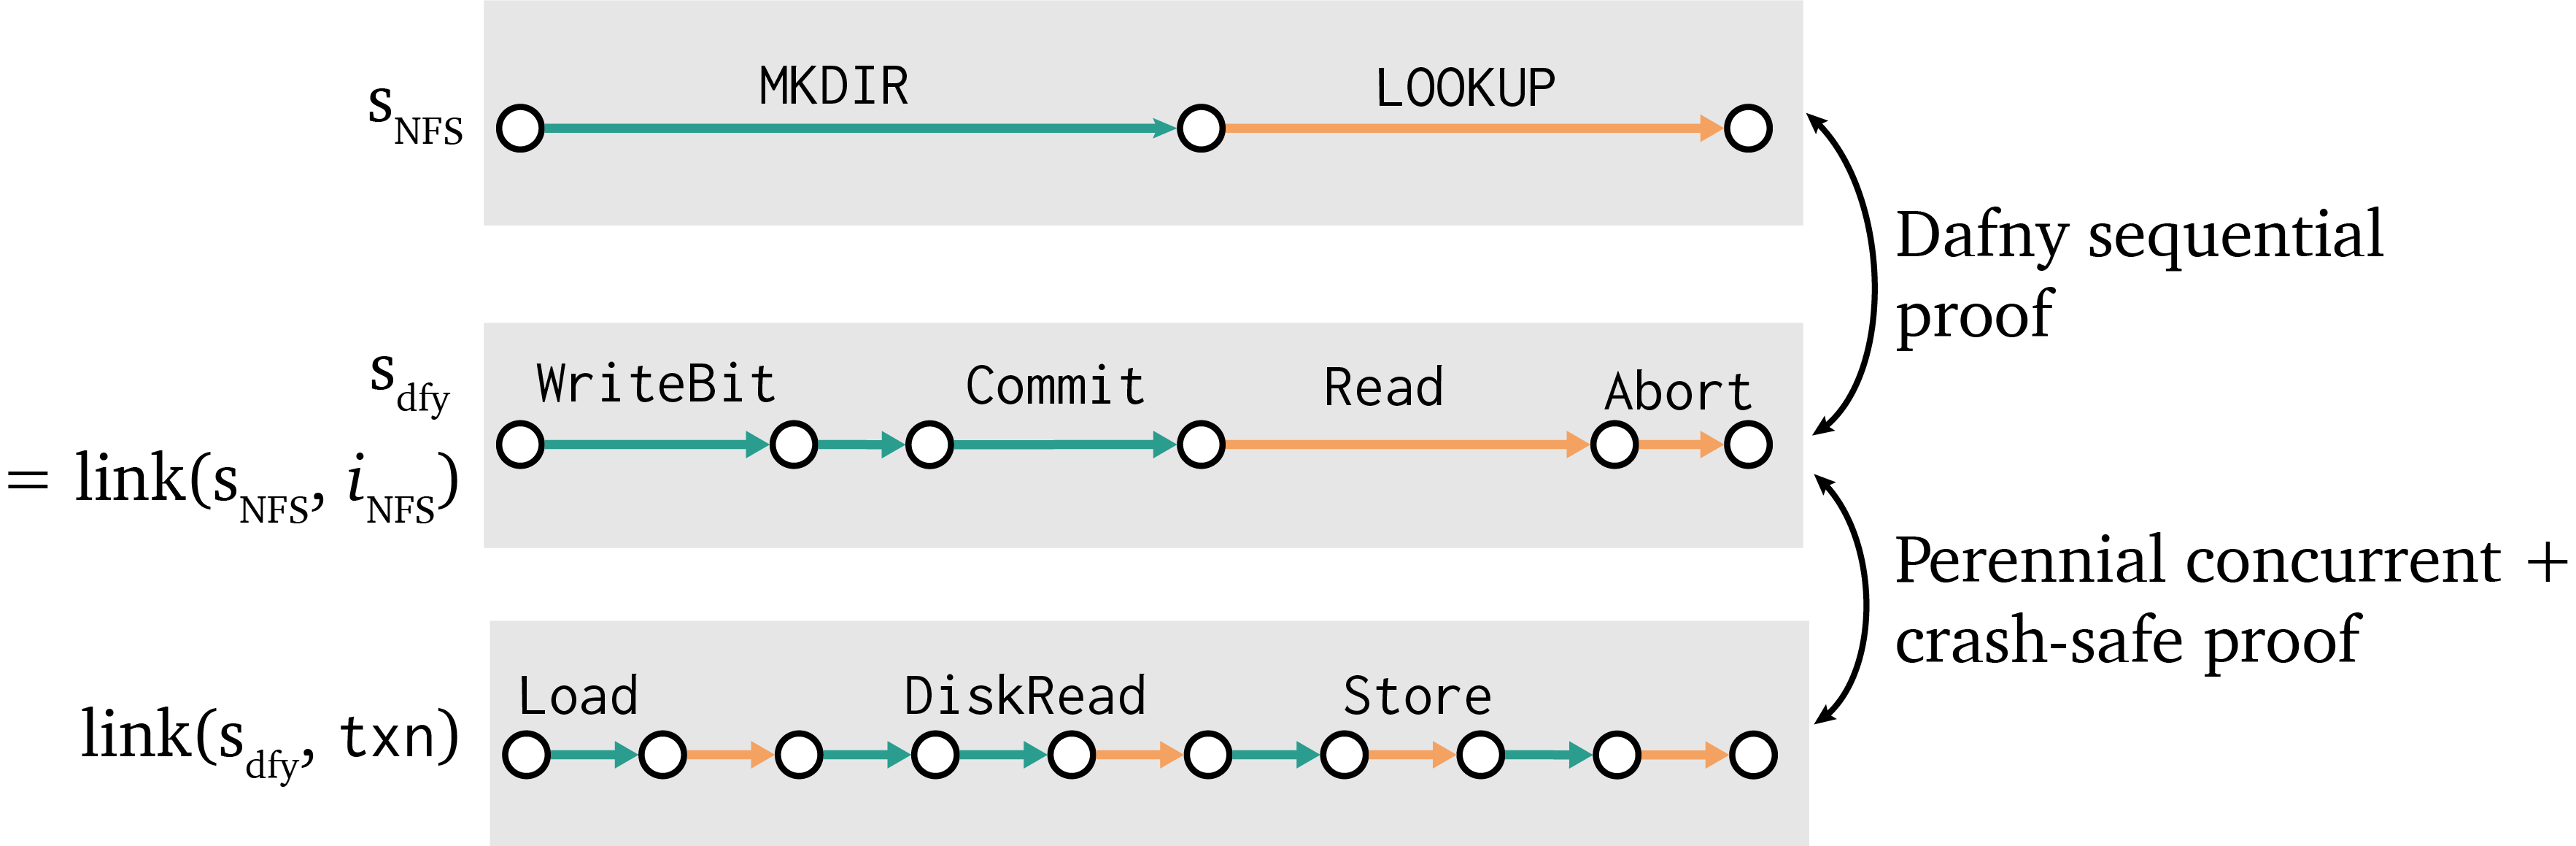
\includegraphics{fig/refinement-execs}
  \begin{center}
  \begin{tikzpicture}[scale=1, >=latex, every node/.append style={}]

  \tikzstyle{txnstate}=[circle,draw,minimum size=2mm,fill=blue!10]
  \tikzstyle{nfsstate}=[circle,draw,minimum size=2mm,fill=yellow!10]
  \tikzstyle{diskstate}=[circle,draw,minimum size=2mm,fill=green!10]
  \tikzstyle{switch}=[->, dashed, dash pattern=on 1.5pt off 2pt]
  \tikzstyle{stepr}=[thick,->]
  \tikzstyle{layer}=[font=\large]

  \setlength{\stepw}{1.25cm}
  \setlength{\dstepw}{\stepw*2}

  \newlength{\nfsbot}
  \newlength{\nfsmid}
  \setlength{\nfstop}{1.5cm}
  \setlength{\nfsbot}{.5cm}
  \setlength{\nfsmid}{(\nfstop+\nfsbot)/2}

  \newlength{\txntop}
  \newlength{\txnbot}
  \newlength{\txnmid}
  \setlength{\txntop}{-.5cm}
  \setlength{\txnbot}{-1.5cm}
  \setlength{\txnmid}{(\txntop+\txnbot)/2}

  \newlength{\disktop}
  \newlength{\diskbot}
  \newlength{\diskmid}
  \setlength{\disktop}{-2.5cm}
  \setlength{\diskbot}{-3.5cm}
  \setlength{\diskmid}{(\disktop+\diskbot)/2}

  \draw node (N0a) at (0,\nfstop) [nfsstate] {};
  \draw node (N1a) at (\dstepw,\nfstop) [nfsstate] {};
  \draw node (N1b) at (\dstepw,\nfsbot) [nfsstate] {};
  \draw node (N2b) at (\dstepw*2,\nfsbot) [nfsstate] {};

  \draw [stepr] (N0a.east) -- (N1a.west) node[midway,above=.2] {\code{LOOKUP}};
  \draw [stepr] (N1b.east) -- (N2b.west) node[midway,above=.2] {\code{CREATE}};
  \draw [switch] (N1a.south) -- (N1b.north);

  \draw node (T0a) at (0,\txntop) [txnstate] {};
  \draw node (T1a) at (\stepw,\txntop) [txnstate] {};
  \draw node (T2a) at (\stepw*2,\txntop) [txnstate] {};
  \draw node (T2b) at (\stepw*2,\txnbot) [txnstate] {};
  \draw node (T3b) at (\stepw*3,\txnbot) [txnstate] {};
  \draw node (T4b) at (\stepw*4,\txnbot) [txnstate] {};

  \draw [stepr] (T0a.east) -- (T1a.west) node[midway,above=.2] {};
  \draw [stepr] (T1a.east) -- (T2a.west) node[midway,above=.2] {\code{Commit}};
  \draw [switch] (T2a.south) -- (T2b.north);
  \draw [stepr] (T2b.east) -- (T3b.west) node[midway,above=.2] {};
  \draw [stepr] (T3b.east) -- (T4b.west) node[midway,above=.2] {\code{Abort}};

  \draw node (D0a) at (0,\disktop) [diskstate] {};
  \draw node (D1a) at (\stepw,\disktop) [diskstate] {};
  \draw node (D1b) at (\stepw,\diskbot) [diskstate] {};
  \draw node (D2b) at (\stepw*2,\diskbot) [diskstate] {};
  \draw node (D3b) at (\stepw*3,\diskbot) [diskstate] {};
  \draw node (D3a) at (\stepw*3,\disktop) [diskstate] {};
  \draw node (D4a) at (\stepw*4,\disktop) [diskstate] {};

  \draw [stepr] (D0a.east) -- (D1a.west) node[midway,above=.2] {\code{Read}};
  \draw [switch] (D1a.south) -- (D1b.north);
  \draw [stepr] (D1b.east) -- (D2b.west) node[midway,above=.2] {\code{Write}};
  \draw [stepr] (D2b.east) -- (D3b.west) node[midway,above=.2] {};
  \draw [switch] (D3b.north) -- (D3a.south);
  \draw [stepr] (D3a.east) -- (D4a.west) node[midway,above=.2] {};

  \draw [align=center] node (NFS) at (\stepw*5.5,\nfsmid) [layer] {$\snfs$ \\ \gooselayer{NFS}};
  \draw [align=center] node (Txn) at (\stepw*5.5,\txnmid) [layer] {$\sdfy$ \\ \gooselayer{Txn}};
  \draw [align=center] node (Disk) at (\stepw*5.5, \diskmid) [layer] {$\linkedcode$ \\ \gooselayer{Disk}};

\end{tikzpicture}

  \end{center}
  \caption[One execution of DaisyNFS at its three abstraction levels]{One possible execution of DaisyNFS, receiving parallel LOOKUP and
    CREATE operations, at its three abstraction levels.
    Within an execution each row is a thread, and dashed arrows indicate
    context switches.
    The proof shows the bottom execution is equivalent to an atomic execution of
    each thread at
    the Txn layer~(in \cref{thm:gotxn-transfer}),
    and sequential reasoning shows each atomic sequence behaves according to the NFS
    specification~(in \cref{thm:dafny}).}
  \label{fig:refinement-execs}
\end{figure}

There are two assumptions needed for the theorems to compose. First,
$\seqrefinement_{\mathrm{dfy}}(i_{NFS})$ should imply $\seqrefinement(i_{NFS})$,
to bridge the assumption and theorem being proven in Dafny. That is, the
encoding of the refinement conditions in Dafny must be correct, but also the
semantics of the transaction system operations modeled in Dafny must match the
Coq proof. Second, every Dafny transaction must be valid, meaning
$\mathrm{safe}(i_{NFS}(op))$. Safety has a static restriction that transactions
should not modify global state, which the Dafny code satisfies because the only
mutable state in the file-system Dafny class is the transaction system, so
file-system operations cannot make mutations other than through GoTxn. The
dynamic restrictions for safety are expressed with preconditions on the GoTxn
interface so that Dafny automatically enforces them.

\tej{subtlety about internal mutable state}

% We have some
% confidence this holds due to a simple check over the Dafny code: the only
% mutable state in the Dafny class that implements the file system is the ghost
% variables and the transaction system, so it cannot make mutations other than
% through GoTxn (ghost variables cannot influence execution due to the design of
% Dafny).

\section{Verifying the Dafny implementation}%
\label{sec:daisy:design}

\Cref{sec:daisy:proof-dafny}
explains how DaisyNFS connects sequential verification in Dafny to concurrency
and crash safety in GoTxn. This instead section focuses on the sequential
verification and file-system design themselves.

% The proof is given by annotating the code with proof steps, which include
% updates to ghost state, assertions to assist the automated verification, and
% calls to lemmas.

DaisyNFS is implemented and verified in several layers of abstraction, depicted
in \cref{fig:dafny-layers}. Each layer is implemented as a class that wraps the
lower layer as a field, until finally the transaction system is an assumed interface in Dafny.
The \cc{daisy-nfsd} binary implements the NFS wire protocol in
unverified Go code and calls the top-level Dafny class and its verified
methods to handle each operation.

\begin{figure}
\small \centering
\begin{tabular}{ll}
  \toprule
  \textbf{Layer} & \textbf{Functionality} \\
  \midrule
  daisy-nfsd & NFS wire protocol. \\
  dir & Directories and top-level NFS API. \\
  typed & Inode allocation. \\
  byte & Implement byte-level operations using blocks. \\
  block & Gather blocks for each file into a single sequence. \\
  indirect & Indirect blocks organized in a tree. \\
  inode & In-memory, high-level inodes; block allocation. \\
  txn & Assumed interface to external transaction system. \\
  \bottomrule
\end{tabular}
\caption{Layers in the Dafny implementation and proof of the file-system
operations.}
\label{fig:dafny-layers}
\end{figure}

The layers of the file system
can be organized into groups that implement three difficult pieces of
functionality: organizing data blocks into metadata and data (the
indirect and block layers), translating byte-level operations into
block operations (the byte and typed layers), and implementing
directories as special files that the file system itself reads and
writes (the dir layer). The modularity was essential to complete the proof in
manageable chunks (to avoid overwhelming the developer and prover), and it would
have been natural even without verification.

\subsection{Implementing the file system using transactions}

The design of DaisyNFS is broadly similar to the file system in xv6~\cite{xv6},
as well as Yggdrasil~\cite{sigurbjarnarson:yggdrasil}, a verified sequential
file system. We also adopt the recursive strategy for implementing and
verifying indirect blocks from DFSCQ~\cite{akonradi-meng}; recursion simplifies
the implementation of triply-indirect blocks, which are needed to reach a
reasonable maximum file size of 512GB.\@ Unlike most file systems, DaisyNFS is designed
to fit every operation into a transaction in order to support our goal of
sequential reasoning. This is a non-standard design and we encountered some
unique challenges in doing so. In this section we highlight difficulties in
fitting two features into transactions: rename and freeing space from deleted
files.

\subsubsection{Rename}
\label{sec:dafny:rename}

The NFS RENAME operation is similar to the \cc{rename} system call: it moves a
source file or directory to a destination location. What makes it tricky is that
it involves more than one inode and hence introduces the possibility for
deadlock.
% , which we would like to avoid even if the theorems do not forbid it.
We
use the standard strategy of enforcing a global ordering where inodes are always
locked in numerical order (smaller inode numbers first); this avoids a deadlock
where a cycle of threads is waiting on each other.

In a rename operation, the source and destination are each specified by a
combination of the parent directory inode and name within that directory. Rename
has an additional functionality of overwriting the destination if the source and
destination are files, or if both are directories and the destination is empty.
It is this latter check that makes deadlock avoidance difficult: it is necessary
to lock the source and destination directories first to lookup the source and
destination names, but those might be files that are earlier in the inode lock
order. We address this in the code by returning an error from the Dafny
transaction before the lock order would be violated. The error comes with the
set of inodes that should have been acquired.  The rename is then re-run with
this set of inodes as a lock hint which are all acquired in the correct
order at the beginning of the operation. The inodes to lock are only a hint and must be compared
against the current source and destination in case those inodes have changed in
the mean time. The rename operation runs in a loop until the lock hint succeeds;
the loop is potentially unbounded, but each iteration can only fail due to
concurrent renames that involve the same inodes.

At this point it is worth discussing the performance considerations that lead to
handling lock ordering in the file
system, rather than generically in GoTxn. The transaction system could
avoid deadlocks by either enforcing a global order over addresses or by
timing-out operations. Enforcing a global order is inefficient for the file
system; data blocks will never cause deadlock because the file system only
accesses a block after locking the (unique) inode that owns it. Timing-out
operations would lead to slow and spurious transaction failures that could more
rapidly be avoided in the higher-level code, hence we do not attempt to detect
deadlock dynamically.


\subsubsection{Freeing space}
\label{sec:dafny:freeing}

Freeing space becomes surprisingly tricky with large files. The problem is that
a large-enough file may reference too many blocks to be
freed in a single transaction. Transactions are bounded by the size of the
on-disk log (which can hold 511 blocks), whereas freeing a file requires
writing 0s to the block allocator for all of its formerly used blocks to mark them as free.
DaisyNFS handles this issue by splitting file removal and space reclamation
into separate transactions. The latter is implemented with an operation
\cc{ZeroFreeSpace(ino)} which frees and zeros the unused space in an inode that
we prove has no effect on the logical file-system state. Because this operation is a
logical no-op, it is safe to call it at any time.

The implementation is careful to call \cc{ZeroFreeSpace} after any operation
that leaves unused blocks, in particular \cc{REMOVE}, which deletes a file, and
\cc{SETATTR}, which can shrink a file by reducing its size. Since
\cc{ZeroFreeSpace} doesn't affect the user-visible data, it can return early to
avoid overflowing a transaction. The unverified code that manages freeing space
runs the operation in a loop until it covers all of the unused space in an
inode.

There is one case where freeing blocks is important for correctness and not just
to reclaim space. Growing a file is supposed to logically fill the new space
with zeros. If the file had old data in that space, it might not be zero but
instead contain previously written and deleted data, which both violates the specification and
is a potential security risk. The way we handle this with background freeing is
with validation: when the \cc{SETATTR} operation grows a file, it checks if the
free space is already zero first, and if not fails with a special error code. The
unverified code uses this error as a signal to immediately call
\cc{ZeroFreeSpace} and try the operation again. The same support also handles
holes created by writing past the end of a file, which are similarly supposed to
be zero.

The freeing implementation is an interesting example of using validation in
verification. The specification for much of the freeing code is loose, allowing
any data to be written to the free space. Only the code that checks if the
zeroing is done needs to be verified against a strong specification. The rest of
the code does still needs to be correct for this check to succeed, but we
aren't required to prove it.

\subsection{Verifying the indirect block implementation}%
\label{sec:dafny:indirect}

DaisyNFS supports large files using indirect blocks. A file's inode has a fixed
number of addresses for block addresses, some of which are used as indirect
blocks that hold another layer of addresses rather than direct blocks that have
file data. A single level of indirection is insufficient for a practical file
system, so DaisyNFS implements support for arbitrarily indirect blocks, and in
practice the file system uses up to triply-indirect blocks to support files up
to 512GB.\@

The indirect and block layers together implement an abstraction of a file as a
sequence of blocks, hiding the fact that some of the blocks are used as
metadata. These sequences are always of the maximum size, and only the next
layer reasons about file sizes. To efficiently represent files of the maximum
size, the code uses a convention that a zero block address is treated implicitly
as encoding a zero block, including for indirect blocks, an idea borrowed from
DFSCQ~\cite{akonradi-meng}. Indirect blocks are implemented recursively, where a
$k$-indirect block is always treated as containing 512 pointers to
$(k-1)$-indirect blocks, and a 0-indirect block contains file data. Zeros are
also treated recursively so that a single zero in an inode for the root of a
triply-indirect block efficiently stores a whole tree corresponding to many
gigabytes of zeros.

An inode has space for twelve 64-bit block addresses, after accounting for space
used by its attributes and type information. In principle all of these addresses
could be uniformly used as triply-indirect blocks. However, this would create a
lot of indirection for small files and lower performance for the common case.
Thus instead of organizing them in this way, the code uses a whole range, with
mostly direct blocks and a handful of indirect blocks. To keep the code general,
the indirection level of each of the twelve blocks is given in a global
indirect-block configuration, and most of the code is generic over the configuration. We currently
configure DaisyNFS with 8 direct blocks, two 1-indirect blocks, a 2-indirect
block, and a 3-indirect block. Just the direct and indirect blocks can address 4
MB fairly efficiently, but the triply-indirect block allows files to be large.

Indirect blocks pose a challenge for verification due to the classic problem of
\emph{aliasing}. The proof must show that modifying a data block or indirect
block has no effect on other files. In the DFSCQ proof, the invariant
captures the non-aliasing between files using separation logic, which makes
disjointness easy to express. In Dafny we have no such logical
technique, so we instead use a standard SMT-friendly trick for the invariant: in
addition to the physical mapping that tracks how to dereference a block address,
the indirect layer proof tracks a ghost \emph{reverse} mapping that tracks where
each in-use block number is stored. The invariant states that the forward and reverse
mappings are inverses of each other, which implies that modifying an address
only affects its owner and nothing else.

To encode the reverse mapping, the code uses a ``position'' datatype \cc{Pos} to
represent the location of a block within an inode. With indirect blocks, the
metadata blocks themselves also need to be considered locations, since the
invariant must also rule out metadata aliasing with data or other metadata. A
\cc{Pos} encodes an inode, an indirection level, and an offset for the blocks at
that indirection level to uniquely identify where a block is used. If we imagine
that an inode's block pointers are organized in a tree, the roots are stored
directly in the inode while the leaves are direct blocks. An indirection level
which is higher than the leaf level describes a metadata block.

The indirect block proof is split into the indirect and blocks layers. In the
indirect layer, the abstract state maps a \cc{Pos} to a block, and separately
tracks the size and attributes of each inode. The invariant also expresses that
the block allocator's used blocks have an associated \cc{Pos} and that the free
ones do not. The interface for the indirect layer exposes reads and writes for
positions, regardless of whether they are metadata or data blocks. The block
layer above instead exposes a map from inode number to a flat sequence of blocks by
mapping each leaf position to its linear index within the inode. Separating
these two made it easier to work on the indirect layer while exposing a much
more natural abstraction of a file as a sequence of blocks for the rest of the
file-system implementation.


% \subsection{Random notes on development process}
%
% \begin{itemize}
%   \item Used inefficient functional Dafny code at first, then slowly migrated to
%         in-memory data structures and improved performance.
%   \item Hard to debug and fix timeouts. Profiling verification performance is
%         hard.
%   \item Profiling Go code is great as usual. The generated code looks strange,
%         but I think after code generation it's pretty ordinary (the weird things
%         are mostly bad variable names, lot of unused assignments, and anonymous
%         functions that are immediately called).
%   \item Used some unit tests, but very few and only at the top level. Mainly
%         debugged Go compilation issues and cases where errors were
%         unintentionally being returned.
%   \item Trusted code isn't easy, had bugs in it before testing it thoroughly.
%         Also violated preconditions in top-level specs, triggering memory-safety
%         bugs.
% \end{itemize}



\chapter{Goose}%
\label{sec:goose}
A key component of any infrastructure for systems verification is the connection
between the proof and the executable code. The rest of this thesis focuses on
crash safety and concurrency as challenges to reasoning about storage systems.
This chapter is about Goose, which solves a more fundamental and practical
problem of reasoning about efficient code.

The basic setup we take for Goose is to first write the implementation in
ordinary Go, automatically translate the code to a model in the Coq proof
assistant, then carry out the proof on top of the model. Goose encompasses is
the entire process: it includes the translation tool itself, the way we model Go
code, and finally the reasoning principles for proving properties of translated
Go. (We will also use ``Goose'' in some places to refer to the subset of Go
supported by the translation tool.)

This chapter is intentionally fairly independent of the rest of the thesis for a
reader interested in verifying Go code but not the specifics of the
transaction-system proof or the file system built on top. Concurrency is
relevant to accurately modeling and reasoning about Go, but crash safety is also
of little importance in this chapter. Crashes are modeled simply by stopping
execution and wiping out all of the state except for the disk, which does not
relate to the specifics of Go.

\section{Goals and motivation}

There are two main goals for Goose: \textbf{flexibility} in writing code and
\textbf{soundness}. Flexibility is a goal so that the developer can write
efficient, high-performance code, as long as the proof engineer can also reason
about it (in this thesis the developer and proof engineer are frequently the
same). Goose is sound if the model captures the behaviors of the code, which is
required for the proofs to say something meaningful about the executable Go
code. If the code could go wrong in some way that the model doesn't capture, we
might finish a correctness proof but still have a bug; soundness makes sure this
doesn't happen.

There are alternate setups for verification where the connection between the
proofs and the code is not given by a model and translation, but the Goose
approach prioritizes flexibility in order to write fast code. The transaction
system sometimes does something efficient to shave off a bit of time, and its
proof pays the price by including a more complex correctness argument.

Soundness isn't a property we can immediately measure, since the translation
might miss subtleties of the source code that we have not noticed. However, the
design of Goose tries to achieve soundness. Sometimes soundness and flexibility
are in tension. In general the tradeoff was in favor of performance, so if the
some language feature is needed for good performance, Goose models it, but if it
is a mere convenience the translator might reject idiomatic code and force the
programmer to do something unusual. The result is that Goose is pleasant and
productive enough to write in, but requires some practice for a Go programmer.

\section{Why Go?}

\tej{need to connect to goals and motivation}

Go turns out to be a very convenient language for building verification
infrastructure. The Goose translator effectively gives a semantics to
the source code, in the form of the semantics of the generated GooseLang
code. For the verification to be meaningful, the translation must
preserve the semantics of the source, or at least over-approximate it.

We needed to build the translator while being careful to capture the
source code accurately. One highly practical aspect of Go is that it has
good tooling, including libraries for parsing and type-checking Go
source code. Not only do these libraries save time in implementing
Goose, they greatly improve reliability since they are written by
experts (the Go compiler team, extracting code from the compiler
itself).

In addition to having an accurate syntax tree and even types for the
source code, Go is a simple language. There wasn't much in the way of
syntax that we needed before the Goose subset of Go was sufficient to
write real systems, and even idiomatic Go didn't require much more than
the basics. The remaining restrictions in Goose were easy enough to work
with that we could implement GoJournal the way we wanted to.

Finally, Go is a good language to build systems in. It has efficient and
useful built-in slice and map collections, and anything we build on top
is verified. The runtime handles concurrency efficiently and has good
support for synchronization using locks and condition variables,
allowing a low-level implementation. We were able to use low-level
interfaces to the operating system to access the disk. Garbage
collection simplifies some code and carries a relatively low performance
impact due to the efficient runtime. The tooling for testing, debugging,
and profiling is extremely good, making it easy to fix bugs (before
verification or in unverified code) and find performance problems while
optimizing.

\section{Related work}
\label{s:goose:rel-work}

There are many approaches and systems people have used to verify
implementations.

We wanted control over the translation process to simplify the resulting
model that we needed to write proofs for. Using an existing translator
that essentially translates syntax would still leave the task of giving
a semantics to the output code and proving the right specifications in
Perennial to reason about various parts of the semantics.

Most closely related work is Robbert Krebbers's thesis, on a semantics
for C that includes both operational semantics and an ``axiomatic
semantics'' which is a separation logic for interactive proofs (it also
has an interpreter to test and debug, which produces all of the
behaviors of a program).

VST also models C for the purpose of interactive proofs.

Extraction in the other direction is sometimes used, particularly for ease of
verification; see Verdi, FSCQ, Fiat, and \fstar. Rather than starting with efficient
code (and requiring the developer to write it), it is possible to instead make
the extraction process generate more efficient code (cite Clement's
fiat-to-facade work).

\tej{Much more to say here}

\section{High-level overview}

\tej{connect this to goals and motivation framing}

The goal of the translation is to model a Go program using GooseLang,
which is a programming language defined in Coq for this purpose. When we
say GooseLang is a programming language, we mean it in a theoretical
sense: GooseLang consists of a type of programs in Coq and a small-step
semantics of these programs. Since GooseLang programs support references
to model the Go heap, the semantics is written in terms of transitions
of (program, heap) pairs where the heap maps pointers to values. The
intention of the translation is that the semantics of the translated
function should cover all the behaviors of the Go code, in terms of
return values and effect on the heap. As long as this is true, a proof
that the translated code always satisfies some specification means that
the real running code will, too.

GooseLang is a low-level language, so many constructs in Go translate to
(small) implementations in GooseLang. This implementation choice proved
to be much more convenient than adding primitives to the language for
every Go construct. For example, a slice is represented as a tuple of
pointer, length, and capacity, and appending to a slice requires
checking for available capacity and copying if none is available.
Appending to a slice is a complicated operation, and it was easier to
write it correctly as a program rather than directly as a transition in
the semantics. The one cost to this design strategy is that an arbitrary
GooseLang program is much more general than translated Go programs. This
has no impact on verifying any \emph{specific} Go program.

The extra generality of GooseLang does have some downsides since at one point in
the development, in the transaction system's specification, we refer to an
arbitrary GooseLang program. This theorem is made a bit more complicated since
to there are some ill-defined GooseLang programs that no Go program could
generate which the theorem needs to exclude. The transaction system
specification uses a standard technique of restricting to well-typed GooseLang
programs, and encoding syntactic restrictions in that type system.

An important aspect of GooseLang is supporting interactive proofs on top
of the translated code. The interactive proofs use separation logic, a
variant of Hoare logic, so specifications describe the behavior of each
individual function. In order to support verification of any translated
code, GooseLang comes with a specification for any primitive or function
that the translated code might refer to, including libraries like slices
used to model more sophisticated Go features. GooseLang has many
``pure'' operations that have no effect on the heap, due to many
primitive data types and operations (for example, there are both 8-,
32-, and 64-bit integers, and arithmetic and logical operations for
each). The specifications for these operations are handled with a single
lemma, which is applied automatically with a tactic \cc{wp_pures}.

Since our goal is to support interactive rather than automated proofs,
it is helpful to make the model simple to work with. We try to maintain
a strong correspondence between the model and source code: each Go
package translates to a single Coq file, and each top-level declaration
in the Go code maps to a Gallina definition (a GooseLang constant or
function). Goose has a special case for translating immutable variables
to let bindings in GooseLang (rather than allocating a pointer that will
only be read). As a result, factoring out a sub-expression to a variable
has little impact on proofs, since it just adds one more pure step.

While the model is simple in terms of control flow and structure, we can
safely translate any given Go operation to a sophisticated model as long
as the proof abstracts it away. The subsequent sections in this chapter
walk through several features of Go. In each case we first implement the
feature in GooseLang, which as a model of its behavior primarily aims to
be faithful to Go. Next, we develop reasoning principles for the
features, in the form of separation logic assertions (for example, to
represent a slice) and Hoare triples (for example, to specify the
behavior of Append). The key is that the model is trusted to capture
Go's behavior so some sophistication is useful, whereas the reasoning
principles aim to hide that complexity to make proofs practical.

\section{GooseLang}

\tej{give a formal description of the target language}

\tej{also need to describe Hoare triples and separation logic, might as well do
that here since it's part of the foundations of reasoning about GooseLang}

\section{Supported and unsupported
features}

Each function is translated to a single Coq definition, which is a
GooseLang function. For concurrency, Goose supports the \cc{go}
statement and the synchronization primitives \cc{*sync.Mutex} and
\cc{sync.Cond}.

Go's primitive uint64, uint32, uint8 (byte), and boolean types are all
supported, as well as most of the pure functions on those types. Goose
also supports pointers, structs, and methods on structs. Finally, Goose
supports Go's built-in data structures, slices and maps.

Notably missing in Goose but prominent in Go is support for interfaces
and channels. We believe both are easy enough to support, but interfaces
were not necessary for our implementation, and rather than channels we
use mutexes and condition variables for more low-level control over
synchronization.

Control flow is also slightly tricky since a Go function is translated
to a single GooseLang expression that should evaluate to the function's
return value. We can support many specific patterns, especially common
cases like early returns inside \cc{if} statements and loops with
\cc{break} and \cc{continue}, but more complex control flow ---
particularly returning from within a loop --- is not supported. If we
wanted to fix this the right solution would probably be to represent all
functions in continuation-passing style, though this would complicate
the translation of every function call.

We do not support Go's defer statement. It would be nice to support some
common and simple patterns, particularly for unlocking, by translating
\cc{defer} statically; Go's general \cc{defer} statement is much more
complicated to model since it can actually be issued dynamically and
pushes to a stack of calls that are executed in reverse order at return
time. This generality is rarely exploited so it would be useful to model even
just uses of \cc{defer} that can be statically analyzed.

We do not support mutual recursion between Go functions, and
additionally require the translation to be in the right order so
definitions appear before they are used. The subtlety here is that
definition management in Go, as in most imperative languages,
conceptually treats all top-level definitions as simultaneous, whereas
Coq processes definitions sequentially. Using Coq definition management
to model Go definition management imposes a limitation compared to Go,
but is much simpler to work with compared to modeling a Go package as a
set of mutually recursive definitions. In such a model it would be
necessary to first give specifications to every definition that may be
assumed by other proofs, and to ensure the proof isn't circular.

\section{Modeling pointers}

Pointers turn out to be slightly subtle because of concurrency. In
short, GooseLang disallows concurrent reads and writes to the same
location by making such racy access undefined behavior (any
specification for a program implies that if the precondition holds, the
program never exhibits undefined behavior). The hardware provides some
guarantees, but they are relatively weak: for example, different cores
can observe writes at different times. Go's own memory model specifies
even weaker guarantees. Rather than attempt to formalize Go's rules
(which are complex and involve defining a partial order over all program
instructions), we side step the issue and make any races undefined,
which works for our intended use cases since we always synchronize
concurrent access with locks.

To disallow concurrent reads and writes we first need to detect them.
The GooseLang semantics does this by augmenting the heap with extra
information giving the number of current readers. Rather than making
reads a single atomic step, we split them into two primitives. The first
increments the number of readers and the second decrements the count and
returns the current value. The semantics of a write are only defined if
there are no readers and undefined otherwise.

Next, we need reasoning principles to abstract away this complexity from
program verification. Separation logic turns out to provide the right
language to reason about racy access. When a thread owns
$l \mapsto v$, we know no other thread can have access to location
$l$, so the specifications for reads and writes are unaffected by the
operations being non-atomic (although their proofs are a bit more
complicated to deal with the new semantics). The only change is that the
Read operation is no longer an atomic primitive but a function that
takes two execution steps. In Iris this means that two threads cannot
share memory with an invariant and must mediate access with a lock,
which transfers ownership of the $l \mapsto v$ for multiple execution
steps.

\section{Modeling locks}

As is typical in Goose, locks are not built-in to GooseLang but modeled
using an implementation based on simpler primitives. Since locks are the
only synchronization primitive, implementing them requires shared
concurrent access, which ordinary pointers do not have in GooseLang.
Instead, the language also includes a primitive atomic compare-and-swap
operation that is only used to implement a model of locks. We could also
use the same operation to model Go's low-level atomic operations, like
\cc{atomic.CompareAndSwapUint64} and \cc{atomic.LoadUint64}, but
have not implemented this yet since we don't have code that uses these
low-level synchronization primitives.

The GooseLang lock model is a simple spin lock, represented as a boolean
that is true if the lock is held. The acquire operation $Acquire(l)$
repeatedly executes $CAS(l, false, true)$ to atomically test that the
lock is false and set it to true if so, while release stores false to
the lock. The implementation as a spin lock is merely an operational
model that captures what the lock does: acquire blocks until the lock is
free and sets it to locked, while release frees the lock. The real locks
we use, Go's builtin \cc{*sync.Mutex}, are more efficient than spin
locks, because the runtime understands how to schedule threads that are
waiting on locks. This scheduling and performance difference is not
visible from the model, which allows any thread to be scheduled after
any atomic operation.

The reasoning principles for locks are more sophisticated than the spin
lock implementation. As is typical in concurrent separation logic, we
associate a \emph{lock invariant} to the lock, which is a predicate that
holds when the lock is free. Because this is a separation logic, we can
also interpret the lock invariant as ownership over some data (for
example, some region of memory); the lock mediates access to this
ownership, handing it out when the lock is acquired and requiring it
back when the lock is released. We prove this specification sound
against the GooseLang spin-lock implementation.

\section{Structs}

One of the first features needed when writing any Go is support for
structs. We treat a struct value as just a tuple of its fields, while
the struct definition gives the names of those fields. This data is
enough to implement constructing a struct from its fields and accessing
a field by name, which we implement in Gallina.

Structs in memory are more interesting than struct values. Structs could
be stored in a single location; due to our non-atomic semantics for
memory, this would be sound even for structs larger than a machine word.
However, this model would be too restrictive: it is safe for threads to
concurrently access \emph{different fields}, just not the same field,
and we actually take advantage of this property (largely to write more
natural Go code; working around this restriction requires splitting
structs up if they are stored in memory).

To support this concurrency, we model a struct in memory with a
flattened representation, with each base element in a separate memory
cell. The flattening applies recursively to fields that are themselves
structs, until a base literal is reached (like an integer or boolean);
base elements are at most a machine word, but can be smaller. When
allocating a new pointer, the semantics flattens composite values and
stores the elements in a sequence of contiguous addresses.

With a flattened representation we need non-trivial code to read a
struct through a pointer, particularly when some of its fields are
themselves flattened structs. We implemented this code by augmenting the
``schema'' that represents a struct type with not only the fields, but
their types as well. The exact types are not important, but we do need
the entire tree of how big each field is and the shape of each field in
order to determine the location and extent of any given field. Using
types to represent these shapes makes the translation much simpler,
since we have access to the type of every sub-expression from the Go
type checker. Any load of a value from memory is translated to a Gallina
LoadTyped macro that takes a Coq representation of the type being loaded
and uses it to determine what offsets to load.

For the purpose of proofs we represent a pointer to an arbitrary type
$t$ with a typed points-to fact of the form $l \mapsto_t v$. This
definition expands to a number of primitive points-to facts, one for
each base element. The specification for loading says
$\{l \mapsto_t v\} LoadTyped(t, l) \{RET v, l \mapsto_t v\}$, which
(much like the non-atomic primitive Load) hides the fact that something
non-atomic is happening and looks like an ordinary dereference.
Similarly, StoreTyped also takes a type, although the specification
requires the caller to prove that the value has the right shape (in
reality it always will because the Go code we translate from is
well-typed).

The payoff of structs being many independent locations is that it is
possible to model references to individual struct fields. From a pointer
to the root of the struct, a field pointer is simply an offset from that
pointer (skipping the flattened representations of the previous fields).
This offset calculation is much like the code to read a struct from
memory, except that it merely computes a single offset rather than
iterating over all the fields and offsets.

The Go language reference specifies that each field acts like an
independent ``variable'' (which is stored in the GooseLang heap when it
is mutable in Go), so this model should accurately reflect the
specification. Moreover modeling structs as independent locations is
also justified as being similar to how the implementation works. Structs
in memory are in reality represented by contiguous memory, and field
access is implemented by computing a pointer from the base of the
struct. The main difference between the physical implementation and the
model is that we use a single, abstract memory location for each field,
whereas the implementation encodes all data into bytes.

Recall that $l \mapsto_t v$ is internally composed of untyped
points-to facts for all the base elements of $v$. In order to reason
about $v$'s fields, we introduce a new struct field points-to fact,
written $l \mapsto_{t.f} v$, which asserts ownership of just field
$f$ of a struct of type $t$ rooted at $l$, and gives that field's
value as $v$. A recursive function gives an ``exploded'' set of struct
fields by iterating over $t$'s fields and $v$ simultaneously. Then,
we give a proof that $l \mapsto_t v$ is equivalent to the separating
conjunction of this exploded list. The result is a convenient lemma for
reasoning about a struct using its fields: in the forward direction, the
equivalence breaks a large typed points-to into individual fields (with
the values computed from $v$), while in the other direction it allows
to prove a $l \mapsto_t v$ by gathering up all the fields.

The struct field points-to is indispensable in proofs, because the
pattern of \cc{x.f} in Go when $x$ is a pointer is in fact a field
load (in C, this would be written \cc{x->f}). The model
for loading a struct field is a function \cc{loadField(x, t, f)}
which is implemented in two steps, first computing the offset to field
$f$ and then dereferencing the computed pointer (in both cases the struct type $t$
describes how to interpret field $f$). Having a field points-to gives
a natural specification for this type of load:
$\hoare{l \mapsto_{t.f} v}{\mathtt{loadField}(x, t, f)}{\Ret{v} l \mapsto_{t.f} v}$.

The lemmas about breaking apart and recombining structs are all proven
against a simpler model of structs that only requires flattening and
offset calculations. In a sense the model is the trusted code, but the
fact that the struct maps-to exploding lemma is true that all of the
expected Hoare triples hold provides strong evidence that the model is
also doing the right thing. For example, the exploding lemma shows that
field offsets are disjoint, since the struct maps-to can be broken into
field points-to facts for each field.

Something to emphasize above: all of the struct code is generic for
struct type $t$, which in the code is concretely the ``schema''
described above, a list of fields and types (the code calls this a
``descriptor'' and uses $d$ as the metavariable, to avoid confusion
with a generic type $t$).

\section{Slices}

One of the most commonly used data structures in Go is the slice
\cc{[]T}, which is a dynamically-sized array of values of type
\cc{T}. Goose supports a wide range of operations on slices,
including appending and sub-slicing; it turns out that the semantics of
mutable slices is non-trivial in Go, resulting in an interesting
semantics and reasoning principles.

A slice is a combination of a pointer, length, and capacity. Slices are
views into a contiguous memory allocation; this view can be narrowed
with sub-slicing operations of the form \cc{s[i:j]}, resulting
in aliased slices. The elements between the length and capacity are not
directly accessible but are used to support efficient amortized appends.
Go's built-in slice operations include bounds checks on all slice
operations and panic if a memory access or sub-slice operation goes out
of bounds.

GooseLang has a primitive for contiguous memory, which we use to model
the allocation underlying a slice (though these are not directly
accessible to Go code, since they do not carry enough information for
bounds checking). On top of these we model slices as a tuple of a base
pointer, length, and capacity.

The GooseLang slice model is directly inspired by the implementation of
slices, including modeling slice capacity. Initially we had a more
abstract model that ignored capacity (which would appear to be just an
optimization), but were surprised to find that this was insufficient to
even accurately model subslicing and appending. Directly modeling slice
capacity was the simplest solution to obtain a model that is faithful to
the Go implementation. The Go language reference isn't specific about
what the slice capacity after various operations should be, so our
GooseLang model picks a non-deterministic capacity in several places
(within appropriate bounds).

The most basic operations on slices are indexing and storing. The
GooseLang model of $s$ is a three-tuple, but for clarity we will refer
to its elements as $ptr(s)$, $len(s)$, and $cap(s)$. The
translation of \cc{s[i]} is essentially a load from
$ptr(s) + i$ (or undefined behavior if this offset is out-of-bounds).
Similarly \cc{s[i] = x} stores to the same location. We
translate Go's \cc{len(s)} directly to $len(s)$. Go also supports
accessing a slice's capacity, but this is rarely used and Goose does not
support it.

The Go \cc{append} operation is the most sophisticated to model. The
behavior of \cc{append(s, x)} where \cc{s: []T} and
\cc{x: T} depends on whether there is extra capacity to store the
new element \cc{x}. If there is capacity, then \cc{x} is stored
there and the append returns a new slice with the same pointer but a
larger length. If there is no capacity, then \cc{append} must
allocate a new slice, copy the existing elements to it, and then store
\cc{x}. In the latter case \cc{append} returns a slice with a
fresh pointer.

The difficulty with Go slices arise when supporting subslicing. Consider
\cc{s[:i]}, where \cc{i} is less than \cc{len(s)}.
Clearly this slice should have the same pointer and length \cc{i},
but what should its capacity be? Surprisingly, the capacity of this
prefix is the full capacity of \cc{s}, which means that the unused
elements of \cc{s[:i]} \emph{include the elements of \cc{s}}
beyond the index \cc{i}. As a result, \cc{append(s[:i], x)}
in fact modifies \cc{s[i]}. GooseLang takes care to model this
behavior by implementing \cc{append} exactly as above, taking into
account that \cc{append(s, x)} might be an in-place operation.

The GooseLang model is specifically designed to be sound by sticking to
the Go implementation as closely as possible, but we want reasoning
about slices to be convenient and high-level, without worrying about
slice capacity directly. The design of GooseLang nicely separates the
model from the reasoning principles --- we verify specifications against
the concrete model, so that only the model is trusted and not the
separation logic specifications.

\newcommand{\sliceRep}{\mathtt{sliceRep}}
\newcommand{\sliceCap}{\mathtt{sliceCap}}

The GooseLang model of slices is based on two abstract predicates:
$\sliceRep(s, l)$ and $\sliceCap(s)$. To model the slice values
themselves we use $s : Slice$ where $Slice$ is a Gallina record; a
function $SliceVal(s) : Val$ converts the Gallina representation to
the GooseLang tuple that the slice model uses. We will only present the
\emph{untyped} version of this specification where $l : list val$, but
GooseLang also has a typed version where $l : list T$ where there is
some (Gallina) function $\mathtt{to\_val} : T -> Val$. The typed version is
practically convenient in proofs but is only a small extension to the
untyped version.

The first predicate $\sliceRep(s, l)$ gives the abstract value of
$s$, the list of values it contains, excluding additional capacity. It
also represents ownership over all these elements, in terms of the
underlying struct points-to facts. We use this predicate to specify
loads and stores:

\[
  \hoareV{\sliceRep(s, l) * i < |l|}%
{\mathtt{s[i]}}%
{\Ret{v} v = l !! i * \sliceRep(s, l)}
\]
\[
  \hoareV{\sliceRep(s, l) * i < |l|}%
 {\mathtt{s[i] = v}}%
{\Ret{v} v = l !! i * \sliceRep(s, l[i := v])}
\]

Next, $\sliceCap(s)$ is an abstract predicate that represents
\emph{ownership over the capacity} of $s$. It is necessary to append,
since appending might need to write to the capacity, but unneeded to
read and write to a slice.
\[
\hoareV{\sliceRep(s, l) * \sliceCap(s)}%
{\mathtt{append(s, x)}}%
{\Ret{s'} \sliceRep(s', l ++ [x]) * \sliceCap(s')}
\]

This specification is fairly simple. In fact, we often use a shorthand
$sliceFull(s, l) = sliceRep(s, l) * sliceCap(s)$ when the proof will
always retain ownership of slice capacity, in which case the spec looks
even simpler. However, the proof is non-trivial, since in one case it
moves ownership from $sliceCap(s)$ to $sliceRep(s', l ++ [x])$
(where $ptr(s') = ptr(s)$), while in the other it constructs a
completely new allocation for $s'$.

The most interesting rules are for subslicing and how they interact with
capacity. Consider \cc{s[:i]} again. While Go has no formal
notion of ownership, our specifications do. We can model the
\emph{value} for \cc{s[:i]} easily enough; call it
$sliceTake(s, i)$ (it simply reduces the length and keeps the capacity
of $s$, as specified by Go). Now we need to decide how ownership of
$sliceRep(s, l) * sliceCap(s)$ should relate to ownership of
$sliceRep(sliceTake(s, i), take(l, i))$. It turns out there are two
possibilities: we can either give up ownership of the remainder of $s$
in exchange for $sliceCap(sliceTake(s, i))$, or we can ignore the
capacity of the subslice and keep
$sliceRep(sliceDrop(s, i), drop(l, i))$. These are incomparable and
unexpressed in the code: the decision is based on whether we intend to
append to the subslice but stop using the old slice, or whether we want
to continue using the remainder of \cc{s}.

Concretely, GooseLang verifies the following entailment for reasoning
about subslicing in terms of the slice model:

$sliceFull(s, l) \vdash sliceFull(sliceTake(s, i), take(l, i))$

This entailment precisely captures how retaining ownership of the
capacity of $sliceTake(s, i)$ requires giving up the remainder of
$s$.

$sliceRep(s, l) \dashv\vdash sliceRep(sliceTake(s, i), take(l, i)) * sliceRep(sliceDrop(s, i), drop(l, i))$

This alternative bidirectional entailment splits $s$ into two parts,
but gives up ownership over $sliceTake(s, i)$'s capacity in exchange
for using those elements in \cc{s[:i]}. From this point it will
not be possible to prove the safety of appending to \cc{s[:i]},
since this would conflict with the separate ownership over
\cc{s[i:]}.

\section{Maps}

After slices, maps are the next most commonly used collection type in
Go. We implement maps as lists of key-value pairs, stored in a single
memory location in reverse insertion order. Go's builtin maps are
\emph{not} thread-safe, so the model enforces single-threaded access by
marking the map as being read while reading from it; this re-uses the
race detection for other pointers to ensure that racy access to a map is
undefined behavior, while allowing concurrent read-read access. Maps
support all the Go operations: insertions, reads (including returning
whether the key is present), \cc{len} to get the number of elements
in the map, deletion, and iteration. Go map iteration is
non-deterministic and in practice random, but we did not model this
since it would be challenging to do so; however, the reasoning
principles for map iteration do not expose an iteration order.

The implementation of maps is the most involved out of any of the Go
primitives. It required directly implementing maps (albeit
inefficiently, using an association list) using recursive GooseLang
code. GooseLang is an untyped language, so our first attempts had basic
errors like missing arguments. We improved our confidence in this
implementation both by testing it and by verifying it. Both of these
essentially rule out type errors (regardless of what specification we give),
and the specification is simple enough
to be a reliable test of behavior. Both simple tests and verification
cover easy mistakes like reading the oldest write to a key rather than
the latest, or duplicate keys during iteration (the implementation must
skip over a key after observing it once).

The proof and specification for maps is relatively easy since they are
non-concurrent, so the proof assumes ownership over the entire map. We
treat a map as a pointer to an abstract map value, a GooseLang value
that encodes the entire map data as a list of key-value pairs. The
specification is based on a pure relation $mapVal(v, m)$ that relates
this encoded value to a Gallina map $m$, which uses \cc{gmap} from
stdpp; for simplicity we use \cc{gmap u64 val} and limit map
keys to integers. Values are not a visible notion to the Go code, since
it always interacts with maps via their pointer, so the specifications
all use $mapRep(l, m) = \exists v, l \mapsto v * mapVal(v, m)$. The
indirection is important, since the Go map value
\cc{m : map[uint64]V} is in fact a reference to a map that is
mutated in-place (unlike a slice, which has both pure data --- pointer,
length, and capacity --- and heap data).

For example,

$\{mapRep(l, m)\} mapDelete(l, k) \{mapRep(l, delete(m, k))\}$

Map iteration has a more sophisticated specification [citation
needed]:

\tej{write down iteration spec}

\section{Testing Goose}

Goose is a trusted component in the entire verification process. For the
overall system's proof to be sound, we rely on the model to produce all
of the behaviors of the Go code; that is, the behaviors of the Go code
(in practice, using the Go compiler) should be a subset of the behaviors
of its translated GooseLang (according to the Coq semantics). As long as
this is case, the proof is sound in that if the modeled system always
satisfies some property the code will, too.

One subtlety in the trust we place in Goose is that it only applies when
Goose translates code successfully, that code compiles in Coq, and the
model has no undefined behavior. If any of these fail, then the proof of
the system would either not be possible or not go through. Therefore the
most important bugs are those where the translation's behavior differs
from that of Go; these can compromise soundness of the system and lead
to a proof that is not borne out in practice.

To increase out confidence in Goose, we implemented a large suite of
unit tests. While these tests check that Goose continues to translate
existing code (and check that the translation has not unexpectedly
change), for soundness the relevant test is to compare Go to the Goose
output. Unfortunately GooseLang is not natively an executable language.
Its semantics is expressed as a Coq relation that specifies how an
expression is evaluated (or gets stuck, indicating undefined behavior).
To test GooseLang code, we implemented an interpreter in Coq, which can
run GooseLang code and produce either an error due to undefined behavior
or a result. While the interpreter is not very efficient, it has good
enough performance to run the Goose unit tests.

The interpreter is an important part of the testing strategy, but
ultimately the comparison is intended to be between Go and the GooseLang
semantics. Thus we verified that the interpreter produces executions in
accordance with the semantics. The correctness theorem is slightly
subtle in that the interpreter produces only one possible execution, but
the non-determinism is only due to the choice of what locations to use
for pointers, which should not affect any visible behavior.

The technical challenge with implementing and verifying the interpreter
is that the semantics uses a convenient but non-executable way of
expressing the order of evaluation. GooseLang is a lambda calculus, so
its semantics is expressed as a transition system between expressions.
It is easy to give the semantics of a primitive at the \emph{head} of an
expression; for example, we can say what $Store(l, v)$ does in a given
heap if $l$ and $v$ are already values (it stores $v$ in the heap
and evaluates to \texttt{\#()}, the unit value). It is also easy to
interpret \emph{pure} reductions like \cc{x + y} where \cc{x}
and \cc{y} are values since the semantics of these pure expressions
is already given as a Gallina function.

The challenge in the interpreter comes from \emph{context} reductions,
which specify how to find a sub-expression within \cc{e} to reduce
if the head is not immediately a value. The code follows a standard
presentation of context reduction using \emph{evaluation contexts}. The
idea is to define a type of evaluation contexts \cc{K} that
represent an expression with a hole; a function $fill(K, e)$, usually
written $K[e]$, fills the hole with $e$. The possible evaluation
contexts give all the context reductions in one compact rule: if $e$
can step to $e'$, then $K[e]$ can step to $K[e']$. Thus the
semantics has a rule that works when any such $K$ exists, while the
interpreter recurses through an expression (in the right order) and
evaluates a sub-expression, then fills it into the context. We prove
this correct, showing that the interpreter and semantics agree on an
evaluation order. (Specifically, the proof shows that the interpreter
produces one of the valid evaluation orders; the semantics is intended
to have a deterministic order, but this is not proven.)

The test suite is structured as a number of test functions, each
producing a boolean. If the test is written correctly, it should produce
\cc{true}, which we test in Go. Then to check the semantics of the
translation, in GooseLang we check that the interpreter returns true for
each test function. While we could compare more sophisticated results
like integers or structs between the two, this strategy is especially
easy to implement, since there is no need to correlate Go and GooseLang
outputs and compare structured data.

The interpreter and test framework was designed and implemented by
Sydney Gibson, and is described in greater detail in her master's
thesis. The thesis includes more details on evaluating the interpreter
itself, for example documenting bugs caught by the test suite and other
bugs that are now part of our regression tests.


\chapter{Perennial}%
\label{sec:perennial}
Perennial is a framework for reasoning about crash safety and concurrency that
we developed in order to verify GoTxn. The main component of Perennial is a
program logic based on concurrent separation logic, with extensions for
reasoning about crash and recovery behaviors.

This chapter describes Perennial's reasoning techniques used in the GoTxn proof.
Perennial is built on top of the Iris concurrency framework, and inherits its
support for reasoning about concurrency; the novelty is in reasoning about
crashes and recovery. Some knowledge of Iris is needed to fully appreciate this
chapter, but the intuition needed to understand the GoTxn chapter should be
clear to anyone.

\section{Primer on Iris and separation logic}

\section{Primer on Iris and separation logic}%
\label{sec:perennial:iris}

A program logic is a formal system for specifying and reasoning about programs.
One of the simplest program logics is Hoare logic, still the basis for much
sequential reasoning today. The judgments of Hoare logic consist of
specifications of the form $\hoare{P}{e}{Q}$, which is interpreted as meaning
``if $e$ is run in a state where $P$ holds and it terminates, then the final
state will satisfy $Q$''. The logic has various rules for proving and combining
these specifications.

\subsection{Separation logic}

Separation logic is an extension of Hoare logic that has proven profitable for
reasoning about heap-manipulating programs with pointers and concurrency
(surprisingly, the same techniques help solve both problems). A good
introduction to the basic ideas of separation logic is found in O'Hearn's
``Separation Logic'' article~\cite{ohearn:seplogic}. This section gives a more
terse overview, especially to introduce the relevant notation.

Separation logic introduces some notation for the logical assertions that
describe the heap. The core assertion to talk about pointers is $p \mapsto v$,
pronounced ``$p$ points to $v$'',
which says that the pointer $p$ when dereferenced has value $v$. The new logical
connective of separation logic is
$P \sep Q$, pronounced ``$P$ and separately $Q$'', which says that the heap can
be divided into two disjoint pieces, one satisfying $P$ and the other satisfying
$Q$. Entailment between propositions is written $P \proves Q$, read as ``$P$
entails $Q$'' or ``$P$ proves $Q$'', which says that in any heap where $P$
holds, $Q$ must also hold.

When working in separation logic, specifications like $\hoare{P}{e}{Q}$ are
generally stated in a ``small footprint'' style where $P$ mentions only the
state $e$ relies on for its execution. This intuition is backed by the
celebrated frame rule, which says that if $\hoare{P}{e}{Q}$ holds, any disjoint
state is unaffected, namely $\hoare{P \sep F}{e}{Q \sep F}$.

Instead of working with Hoare triples, it is convenient to instead define
specifications in a different style of \emph{weakest preconditions} (WPs). We will use
$\wpre{e}{Q}$ to denote the weakest precondition of $e$ with postcondition $Q$;
if $e$ is run in a state satisfying $\wpre{e}{Q}$ and terminates, the final
state will satisfy $Q$. Note that the $\wprew$ is a \emph{predicate over
states}, not a judgment of the logic like a Hoare triple. To build intuition, the statement
$P \proves \wpre{e}{Q}$ is equivalent to $\hoare{P}{e}{Q}$. An excellent
comparison between weakest preconditions and Hoare triples can be found in
``Separation logic for sequential programs''~\cite{chargueraud:seq-seplogic}.

The term ``weakest precondition'' is because $\wpre{e}{Q}$ is supposed to be the
\emph{weakest} predicate that implies $Q$ holds after $e$'s execution, in the
sense that any other precondition would imply $\wpre{e}{Q}$, but our work does not
emphasize this aspect of weakest preconditions. Furthermore the literature will
sometimes distinguish between weakest liberal preconditions that only guarantee
$Q$ if $e$ terminates and reserve the term weakest preconditions for a predicate
that also guarantees termination. This thesis uses the term weakest precondition for the
``liberal'' version (also called \emph{partial correctness} as opposed to
\emph{total correctness}), because proving termination in the presence of
concurrency is quite challenging.

\Cref{fig:wp-rules} shows some basic rules of separation logic, phrased in terms of weakest preconditions.
As an example, the frame rule becomes
\ruleref{wp-frame} in terms of the \wpw assertion. Reading this rule forwards, if in a proof
the assumptions include $F$
and separately $\wpre{e}{Q}$, then the proof can move $F$ to the postcondition because
separation logic guarantees the proof of the WP does not affect or invalidate
the part of the heap covered by the frame $F$.

\begin{figure}
\begin{mathpar}
\inferH{wp-frame}%
{}%
{F * \wpre{e}{Q} \proves \wpre{e}{F * Q}}

\inferH{wp-mono}%
{P \proves P' \and \forall v.\, ([v/x] Q' \proves [v/x] Q) \and \hoare{P'}{e}{Q'}}%
{\hoare{P}{e}{Q}}

\inferH{wp-seq}%
{\hoare{P}{e_1}{Q} \and \hoare{Q}{e_2}{R}}%
{\hoare{P}{e_1;\, e_2}{R}}

\inferH{wp-load}%
{}{\hoare{p \mapsto v}{\load{p}}{\Ret{v} p \mapsto v}}

\inferH{wp-store}%
{}{\hoare{p \mapsto v}{\store{p}{v'}}{p \mapsto v'}}

\end{mathpar}
\caption{Selection of proof rules for sequential separation logic.}
\label{fig:wp-rules}
\end{figure}

\subsection{Ghost state and concurrency in Iris}
\label{sec:perennial:concurrency}

Concurrent separation logic~\cite{brookes:csl} generalizes separation logic to
also reason about concurrency. Iris is a type of concurrent separation logic,
with several advances beyond the original formulation. A full
explanation of the Iris logic is out-of-scope for the thesis; ``Iris from the
ground up''~\cite{jung:iris-jfp} is a comprehensive introduction while the
original ``Iris 1.0'' paper~\cite{jung:iris-1} is a shorter introduction for a
reader already familiar with separation logic. Two features of Iris are most
relevant since they are used in the GoTxn proof: ghost state and invariants.

A key technique in Iris is to verify a program by augmenting its
physical state (local variables and the heap) with some additional \emph{ghost
state} which is maintained only for the sake of the proof and has no effect on
the program's execution (hence the term ``ghost''). It is easier to understand
ghost state via its API in Dafny as a programming-language feature, so let
us first see how they help there and then return to Iris.

In Dafny, a variable can be marked \cc{ghost}. Ghost variables can be written
and read in the proof, but Dafny enforces that the ghost variables' values never
influences execution; they can only be used to inform uses of lemmas,
assertions, and other proof annotations. Then at run time ghost variables and all
uses of them are \emph{erased} before running the program. Why would adding a
ghost variable to a program help with its proof? The simplest examples are code
where a ghost variable holds the old value of some variable, say prior to a
loop; this lets the proof refer to the old value while clarifying that the
regular execution does not need it.\footnote{For a concrete example, see the
bubble sort example in
\url{https://www.doc.ic.ac.uk/~scd/Dafny_Material/Lectures.pdf}.}

\pagebreak[1]
Ghost variables can also be used to give abstract specifications to a piece of
code. For example, consider a ``statistics database'' that maintains the running
mean of a sequence of numbers (written in Go for readability):
\nopagebreak
\vspace{\baselineskip}
\hrule\nopagebreak
\vspace{-12pt}\nopagebreak
\noindent\begin{tabular}{p{0.5\textwidth} p{0.5\textwidth}}
\begin{minted}[frame=none]{go}
type StatDB struct {
  count int
  sum   float64
}

func (db *StatDB) Add(n float64) {
  db.count++
  db.sum += n
}
\end{minted}
&
\begin{minted}[frame=none]{go}
func (db *StatDB) Mean() float64 {
  if db.count == 0 {
    panic("empty db")
  }
  return db.sum/db.count
}
\end{minted}
\end{tabular}
\vspace{-8pt}
\hrule
\vspace{\baselineskip}

The code only tracks the count of elements and
their sum, but the behavior of the library is easiest to state in terms of the list of all
numbers added. Thus in Dafny such a library can use a ghost variable to track
the full database, relate this ghost variable to the physical variables
of the code, and then prove that the code returns the correct running mean in
terms of the ghost state.

One intuition for the technique of ghost variables is that it augments the
execution of the program with additional information, which is used only for the proof
and thus not tracked at run time. For every actual execution, there is a
corresponding execution where the ghost variables are maintained and updated.
The proof is carried out on this augmented execution,
but the proofs apply to the normal execution because by design they have the
same behavior. Verifying the program with ghost
variables is easier because the ghost variables can track important
information about the history of the program, such as in the example above of
the pre-loop values of the local variables.

In Iris, the proof is a separate entity from the code. The program logic still
has a way to use ghost variables, with proof rules that construct and update a
ghost variable, applied at the appropriate points in the proof rather than added
to the code. The high-level idea for why this works --- that there is an
augmented execution with the ghost variables ---
remains the same. In fact in Iris it is more obvious
that the ghost variables do not affect program execution, since their creation
and updates only appear in the proof.

So far, we've explained ghost state in terms of ghost variables, with the familiar
API where they can be read and written. Iris ghost state is a bit more
sophisticated in order to support concurrency reasoning. Iris has
separation logic assertions for \emph{ownership} of ghost state, which can be
split and divided among threads. In conjunction with this analogy to ownership,
in concurrent separation logic a piece of ghost state is also referred to as a
\emph{resource} that a thread can own by having an assertion over the ghost
state in its precondition.  A key principle in concurrent separation logic is that in
a proof about a thread of interest, any resources or ownership in that proof's
precondition can never be invalidated by the actions of other threads. Ghost
state can have restrictions on how it may be updated to reason about a shared
protocol that all threads respect.

\newcommand{\dashedbox}[1]{\boxedassert[densely dashed]{#1}[]}
\newcommand{\ghostvar}[2][]{\dashedbox{\gamma \mapsto_{#1} #2}}

A simple example to illustrate both principles is Iris's fractional ghost
variables. The assertion $\ghostvar[q]{v}$ says that the ghost variable $\gamma$ has value
$v$ (of any fixed type) and asserts ownership over a (positive) fraction $q$ of
it --- any fraction $q < 1$ represents read-only access to the ghost variable,
while full ownership $q = 1$ allows writing as well.
Full ownership $\ghostvar[1]{v}$ is common enough that it is often
abbreviated to
$\ghostvar{v}$, with no fraction. The dashed box around this assertion emphasizes that this
assertion is about ghost state and not about the heap, as in the points-to
assertion $p \mapsto v$.  There are several rules for manipulating and
using this fractional ghost state:

\begin{mathpar}
  \inferH{frac-alloc}{}%
  {\proves \upd \exists \gamma.\, \ghostvar[1]{v}}

  \inferH{frac-update}{}%
  {\ghostvar[1]{v} \proves \upd \ghostvar[1]{v'}}

  \inferH{frac-split}{}%
  {\ghostvar[q_1 + q_2]{v} \provesIff \ghostvar[q_1]{v} \sep \ghostvar[q_2]{v}}

  \inferH{frac-agree}{}%
  {\ghostvar[q_1]{v_1} \sep \ghostvar[q_2]{v_2} \proves v_1 = v_2}

  \inferH{upd-fire}%
  {P \proves \wpre{e}{Q}}%
  {\upd P \proves \wpre{e}{Q}}
\end{mathpar}

The new notation $\upd$ is an Iris \emph{update modality}. The assertion
$\upd P$ expresses ownership of resources which could be used to become $P$ with
some update to ghost state. As an example of proving an update modality,
\ruleref{frac-alloc} shows that starting with no assertions it is possible to
allocate a new ghost variable $\gamma$ with value $v$ and complete ownership
over it; this is analogous to how the Hoare triple for allocation has no
precondition. The formal rule that allows the user to get access to $P$ is
\ruleref{upd-fire}. It corresponds to advancing the proof of $\wpre{e}{Q}$ by
changing whatever ghost state is needed to turn $\upd P$ into $P$. As long as
the user of the logic is proving a weakest precondition as the goal, they can
apply this rule to ``eliminate'' an update modality.

Fractional ghost state can be updated after creation with \ruleref{frac-update}.
The update requires full ownership. Fractional ghost variables can instead be
split into smaller pieces with \ruleref{frac-split}; these pieces can no longer
be updated (since this would invalidate the rest of the assertions), but two
assertions for the same ghost variable must be for equal values
(\ruleref{frac-agree}) since the underlying variable has only one value.
Fractional ownership expresses a simple protocol among threads where when a
thread owns a fraction less than one, it can read but not write, and full
ownership is sufficient to write to a ghost variable.

This thesis describes a few constructions for ghost state to carry out parts of
the GoTxn proof, such as the example of fractional ghost state described above. In reality all
ghost state in Iris is defined using a single, general mechanism. Ghost state
can come from any instance of an algebraic structure $M$ called
a ``resource algebra'', where ownership really means
ownership of an element $a \in M$. This thesis does not explain the details of
how ghost state is constructed using resource algebras --- see
``Iris from the ground up''~\cite{jung:iris-jfp}. For the ghost
state in this thesis, we will only give the API, in terms of resources and
rules that allow updating those resources. The Iris logic ensures that the
updates are ``sound'', enforcing a global property that updates to a resource in
one part of the proof never invalidate resources owned by concurrent threads at
the same time.

\begin{figure}[ht]
  \begin{mathpar}
    \inferH{wp-inv-alloc}%
    {P \sep \knowInv{}{R} \proves \wpre{e}{Q}}%
    {P \sep R \proves \wpre{e}{Q}}

    \inferH{inv-atomic}%
    {\atomic(e) \and R \sep P \proves \wpre{e}{R \sep Q}}%
    {\knowInv{}{R} \sep P \proves \wpre{e}{Q}}

    \inferH{wp-fork}%
    {P \proves \wpre{e}{\TRUE} \and Q \proves \wpre{e'}{R}}%
    {P \sep Q \proves \wpre{(\operatorname{fork} \{e\}; \, e')}{R}}
  \end{mathpar}
  \caption{Key concurrency rules in Iris for invariants and forking}
  \label{fig:invariants}
\end{figure}

A fundamental reasoning principle for concurrency is the notion of an
\emph{invariant}. Threads eventually do share state, and invariants
are the main way to reason about how threads coordinate on that shared state.
The assertion $\knowInv{}{I}$ expresses the knowledge that
$I$ is an invariant. Once this invariant is established, the
proof rules in Iris guarantee that $I$ holds at all steps of the program. A
thread that has $\knowInv{}{I}$ in its precondition can make use of the
invariant by ``opening'' it to obtain ownership over $I$, but only for a single program step; it must be
returned afterward to guarantee the invariant holds for other threads. Finally,
invariants are freely \emph{duplicable} --- that is,
$\knowInv{}{I} \proves \knowInv{}{I} \sep \knowInv{}{I}$ --- reflecting that
knowledge of an invariant, once it is established, is an assertion that all
threads agree on which cannot be invalidated.

The formal rules for using invariants in Iris (which are all valid rules in
Perennial) are given in \cref{fig:invariants}. To create an invariant
$\knowInv{}{R}$, a thread gives up $R$, as given in \ruleref{wp-inv-alloc}. The
rule for using an invariant is \ruleref{inv-atomic}, which can only be used over
an ``atomic'' instruction $e$. Perennial is defined for a general language, as in
Iris, and the semantics of the language defines what is modeled to be atomic.
Formally $\atomic(e)$ says that the expression $e$ reduces to a value in a
single reduction step, so that other threads cannot run in between. See
\cref{sec:goose:semantics} for the details on the specifics of what GooseLang
makes atomic.

Ownership transfer is reflected in the rule for forking new threads,
\ruleref{wp-fork}. If a thread has $P \sep Q$ in its precondition, it can pass
some of those resources $P$ to a newly-forked thread and retain the remainder
$Q$ for the subsequent code. Note that due to the separating conjunction these
resources must be separate, so that the rules of the separation logic guarantee
$e$ cannot invalidate $Q$ using its resources $P$. However, invariants give a
way for the two threads to safely share resources: both can have access to
$\knowInv{}{I}$ because the knowledge of the invariant can be duplicated, which
is sound because each thread only uses $I$ for an atomic step and then
guarantees $I$ holds for concurrent threads.

% \tej{Look at Perennial 1.0 paper and Later Credits paper for some inspiration on
% introducing Iris}


\section{Crash weakest preconditions}

Introduce WPC and its meaning

crash framing

Most important rule: allocating an invariant cancels from the crash invariant
(encoding Perennial 1.0 reasoning)

Crash-aware locks (shouldn't really need crash borrows, only use them as part of
2PL proof because the code doesn't open and close the locks in a bracketed way)

\section{Recovery reasoning}

WPR and idempotence rule

generation numbers to explain how resources transition across a crash
(post-crash modality helps make this concrete in the form of a theorem)

In practice, recovery is the thing that sets up the invariants, cancels from its
crash condition, and then always starts up with the contents of those
invariants due to the recovery idempotence rule.

\section{Soundness}

explain how a soundness theorem relates a WPR to a statement about repeated
execution

mention that a bunch of complexity is hidden in proving that soundness theorem,
some coming from Iris base logic and some from the definition of WPC, but we
won't explain it

\section{Reasoning techniques using Perennial}

Using invariants in clever ways, for both standard concurrency reasoning and
crashes

Logically-atomic crash specs expose atomic updates to the state of a module

Notion of a ``durable'' resource via post-crash modality + combining with an
invariant

Refinement reasoning uses lower-level tools from Perennial for a different
soundness theorem


\chapter{Transaction system}%
\label{sec:txn}
The transaction system is the most challenging part of implementing and
verifying DaisyNFS.

\section{Introduction}


Storage systems, such as file systems, need to be carefully structured
to not lose persistent user data, even in the face of application and
whole-system crashes. They often achieve this \emph{crash safety}
property by delegating writing to storage to a \emph{journaling
system}, which exposes an API for executing an operation such that its
writes appear on disk atomically. The journaling system simplifies
implementing the storage system's logic: to atomically modify a set of
objects, the file system simply writes to them one at a time within a single
journal operation.  The result is that each storage operation is atomic with
respect to crashes.

While a journaling system exposes a simple API, its implementation must address
crash safety and also be concurrent for good performance.
Maintaining correctness in the presence of both concurrency and crashes is
challenging.  For example, in pursuit of performance, journaling systems
often avoid holding locks while performing I/O, but reasoning
about the correctness of such optimizations requires considering what
happens if one thread's disk reads interleave with another thread's
disk writes, and what happens when the system crashes anywhere
during that interleaving.

% \mfk{we should make clear that \txn is a Go package.}
This paper presents \txn, a Go package that provides the first formally verified concurrent journaling
system. To verify \txn, we developed Perennial 2.0, an extension to the Perennial~\citep{chajed:perennial} framework
with several features designed to enable modular reasoning about concurrent, crash-safe systems.
In this work we set a goal of giving
\txn a specification that \emph{reflects the simplicity of using a journal for
crash atomicity}.
\txn can be used by an application like a file system or a key-value
store. As long as the application follows a locking discipline
for its on-disk state, such as per-file locks for a file system, proving the correctness
and crash-safety of that implementation on top of \txn should involve
largely \emph{sequential} reasoning, despite the fact that the application
has multiple concurrent threads and can crash at any time.

Realizing this goal raises two challenges: specifying \txn in a way that makes
application reasoning sequential, and proving \txn's implementation correct. The
specification makes reasoning about an operation sequential with a
\emph{lifting} interface where the proof has an abstraction of a ``checked out''
private fragment of the disk that the operation appears to synchronously modify.
At commit time the private fragment is ``checked in'', at which point it is
durable and can be exposed to other threads. The journal guarantees the
operation is atomic by delaying all writes to commit time, so the developer
should not need to explicitly reason about crash safety until commit time.
Perennial 2.0 supports a new technique called \emph{crash framing} to formalize
the intuition that during an operation the developer need not explicitly
consider crash safety.

The second challenge lies in proving \txn itself.  This is
difficult because we desire modularity to make the system's proof tractable,
which requires giving suitable specifications to the internal interfaces of the system.
While the user-visible interface of \txn is simple, the
internal interfaces of a high-performance journaling system are
hard to specify and fit together.
To address this challenge, Perennial 2.0 contributes \emph{logically atomic crash
  specifications} which enable natural specifications of system layers in terms of
a transition system with
atomic transitions for the public methods.
These specifications include a \emph{crash transition}
to describe what happens to the state of a layer during a crash.
% These specifications both intuitively correspond to atomicity
% and are precise enough
Such specifications make it possible to build upper layers of the system on top without
worrying about implementation details of how atomic transitions are achieved.
This separation of concerns lines up with the modularity in the implementation;
the proof layers divide up the reasoning along the same lines that the
code divides up functionality among Go packages.
% Furthermore, we needed
% to incorporate a \emph{crash transition} into the transition system to specify exactly
% what data can be lost on crash, since some of the internal APIs of \txn buffer
% data in memory before persisting it. \mfk{I don't understand this last
%   sentence. And, I would like to avoid another ``we''}

% The internal API makes it difficult to achieve the desired strong
% specification of atomic transactions. The reason the strong specification
% holds is due to the use of locks to protect disk-object ownership. Under
% these ownership assumptions, the journaling system can prove that the
% internal APIs behave atomically with a single logical commit point.

% We implemented \sys on top of Perennial~\cite{chajed:perennial}, a
% concurrent crash-safe verification framework.  We then implemented
% \txn and used \sys to formally specify and prove its correctness and
% crash safety; in the process of doing so we found one design bug that
% was not caught by unit tests (\S\ref{sec:eval:bugs}).

The contributions of this paper are (1) \txn, a concurrent
journaling system with a machine-checked proof of correctness and
crash-safety; (2) the Perennial 2.0 framework, with extensions to the original
Perennial framework that enable modularity and crash-free reasoning on top of \txn;
and (3) \simplenfs, a verified core of an NFSv3 file server built on
top of \txn.

Although \txn is advanced enough to support a high-performance NFS
server, it has some limitations.  \txn's internals (code and proof)
support deferred durability, but for simplicity, \txn's top-level
specification requires applications to immediately flush committed
journal operations, which is sufficient to prove \simplenfs.  \txn is also
less general than JBD2 (e.g., \txn does not support floating commit
blocks), and less general than database transaction systems (e.g.,
\txn does not support undoing journaled operations).

%%% Local Variables:
%%% mode: latex
%%% TeX-master: "paper.tex"
%%% End:

To the best of our knowledge, \txn is the first verified concurrent,
crash-safe journaling system. The verification of \txn builds on a
large body of previous work, as described in the rest of this
section.

\subsection{Perennial 2.0 vs Perennial 1.0}

The verification approach we take is based on a new version of our earlier
Perennial~\cite{chajed:perennial} framework, so we draw a contrast between the
two here. The new implementation is
conceptually similar in that it supports reasoning about concurrency and
crash-safety, it is implemented on top of the
Iris~\citep{jung:iris-jfp,jung:iris-1} concurrency verification system,
and it uses Goose~\cite{chajed:goose-coqpl} to enable verification of Go
programs by translating them into a model in Perennial 2.0.
However, to make verification of \txn feasible, we had to re-write many core parts of the framework.
To clarify which framework is being referenced we will write Perennial 1.0 for the
original framework and Perennial 2.0 for the new one in this section, in order
to highlight the new features Perennial 2.0 supports. The rest of the paper
generally refers only to Perennial 2.0.

%Perennial 1.0 supported verifying Go programs with a system called
%Goose~\cite{chajed:goose-coqpl} that translates Go into a model in Perennial.
%Perennial 2.0 also comes with a new version of Goose that supports the new
%verification infrastructure and extends translation to cover additional features
%in Go used in \txn.



Some of Perennial 2.0's features are needed to support the \txn top-level
specification and enable verification on top of this interface. The reason this
problem is complicated is because the journal does not make operations
automatically atomic but requires the caller to correctly manage ownership, and
Perennial 1.0's refinement specifications do not give a good way to talk about
ownership. The top-level specification of \txn relies on \emph{crash
framing}~(\autoref{s:design:crashframe}) and \emph{crash-aware
locks}~(\autoref{s:design:crashlock}) to enable application proofs that reason
about ownership of durable data.

Perennial 2.0 also scales to a larger system than the mail server verified in
Perennial 1.0. One of the challenges with the larger system is that it has many
internal layers that need their own specifications, so that the proof can be
carried out modularly. Normally a separation logic or refinement-based
specification would be sufficient, but we need internal specifications that capture
the crash and concurrent behavior of each internal library. To that end
Perennial 2.0 incorporates a new specification style which adds \emph{crash
atomicity} to the logically atomic specification styles developed in earlier
work~\citep{jacobs:logatom,svendsen:hocap,pinto:tada}. Modularity in the proof
was necessary to scale verification to
all of \txn's performance optimizations and concurrency.
At the same time, \txn's specification allows
the proof of \simplenfs to mostly avoid reasoning about crashes.

%% The specification for the simple NFS server is based on closely reading RFC
%% 1813~\cite{RFC:1813}, which defines the NFSv3 API in English prose. We do not
%% attempt to formalize all allowed behaviors in the specification, but did attempt
%% to write a formal specification in Coq which would meet the prose specification.
%% \mfk{maybe say we have some confidence in our formal spec, because
%%   \simplenfs can be mounted and used by a linux client.}

%% \joe{talk about JBD2 here}

%% Lifting and disk-object ownership are
%% new techniques that would not more complicated in Perennial due to the
%% need for leases. Perennial does demonstrate a complex example that
%% requires recovery helping to prove correct; our framework does not
%% support this pattern, but we did not need it to prove \txn or the file
%% system since no helping is involved.

%% The most obvious difference to Perennial is the difference in verified artifact:
%% we prove \txn, a \gotxnLOC-line, high-performance transaction system with interesting
%% crash safety and concurrency challenges, along with a \simplenfsLOC-line NFS server using
%% it; Perennial verified a 150-line mail server. Besides simply having much more
%% code, \txn is verified in several modular layers, with four internal APIs, and
%% then we use the specification to verify an application. Perennial did not
%% explain or demonstrate a modular verification story; our contribution of
%% logically atomic crash specifications allows us to scale verification to this
%% larger system by specifying internal APIs, which are more complex than the
%% client-visible one.

%% Perennial did not include explicit crash conditions, instead carrying out all
%% crash reasoning using an invariant. This works for small examples but is
%% inconvenient for modular verification. We instead build on a framework that uses
%% Iris but augments Hoare logic specifications with a crash condition, in the
%% style of FSCQ's Crash Hoare Logic, but extended to support concurrency.

% \subsection{Related verification efforts}

\subsection{Related verification frameworks}

\paragraph{Crash-safe systems.}

% Perennial 2.0's atomic crash specifications enable \txn to formalize the crash behavior
% of a layer in a lightweight fashion---that is, promising that a layer does not
% expose any unexpected intermediate states after a crash.
Any crash-safe system
must reason about the possible states after a crash, and several prior works
have formalized this in different ways for \emph{sequential} crash-safe systems.
FSCQ~\cite{chen:fscq,chen:dfscq} uses Crash Hoare Logic (CHL) to specify crash
behavior through a crash condition, which describes the state of a system if a
crash happens during execution of a function. Alternatively, a number of systems
verify crash safety using refinement
reasoning~\cite{sigurbjarnarson:yggdrasil,ernst:crash-refinement-asms,chajed:argosy,hance:veribetrkv},
but none support the combination of concurrency and crash-safety.

% However, refinement-based proofs can require additional layers for proof purposes
% that do not correspond to modules in the original code.

% However, refinement based proofs can be heavy-weight because they require
% formalizing the entire set of operations that can be performed at every layer of
% a refinement proof (including logically orthogonal operations like allocating
% memory, accessing data structures, and calling other libraries).
% \ralf{I don't understand the last sentence. It seems to be specifically about CSPEC, not refinement proofs in general?}

Although they are not concurrent, some of these systems address other
aspects of performant storage systems that are not found in \txn.
DFSCQ~\cite{chen:dfscq} verifies a high-performance file system built
on top of a logging system with asynchronous disks and log-bypass
writes, which are challenging optimizations that \txn does not
support. VeriBetrKV~\cite{hance:veribetrkv} verifies a key-value store
based on B\textsuperscript{$\epsilon$} trees, a data structure that also underlies BetrFS~\cite{jannen:betrfs}. \txn
and \simplenfs use simple data structures;
the challenge lies in accounting for concurrent accesses.
%where the challenge is concurrent access.
% concurrent access to these structures.

% The proof technique uses refinement between layers
% in a way that is lighter-weight and more flexible than in CSPEC,a and
% additionally uses the crash guarantees of one layer to prove the crash
% guarantees of a higher layer. VeriBetrFS is implemented in Dafny, which has
% tight integration with Hoare logic; this makes it easier to use but also harder
% to extend, particularly with concurrency. In Coq the program logic is not
% built-in, which gives the flexibility to implement a new logic (as FSCQ did) or
% to extend an existing one (as we do on top of the Iris program logic).

\paragraph{Concurrent systems.}

In addition to specifying behavior at intermediate crash points, Perennial 2.0's
specifications describe the atomic commit points of concurrent operations. A
range of verification techniques have been used to address this kind of
challenge in concurrent systems. AtomFS~\cite{zou:atomfs} uses a framework
called CRL-H (concurrent relational logic with helpers) to verify a concurrent
in-memory file system implemented in C. Refinement-based systems such as
CSPEC~\cite{chajed:cspec}, Armada~\cite{lorch:armada}, and Concurrent
CertiKOS~\cite{gu:certikos-ccal} typically prove that a function implements an
atomic operation at a more abstract layer.
However, in \txn, many internal APIs provide operations that are only atomic if
the caller owns some data. This kind of conditional atomicity is easy to express
in Perennial 2.0 using separation logic, but hard to express
as a precondition in a transition system.
% Additionally, as with using refinement for crash-safety reasoning, refinement-based approaches often introduce extra layers for proof purposes. On the other hand, proofs of refinement between
% layers in an SMT-based system like Armada are automated, while proofs are
% interactive in Perennial 2.0.

% Armada~\cite{lorch:armada} also verifies C code but uses a different approach
% based on several layers of refinement between levels, which are progressively
% more abstract versions of the code. Neither of these frameworks
% supports crash-safety guarantees, and neither supports modular verification of a
% lower-level layer independently of upper layers that use it.


\paragraph{Concurrent, crash-safe reasoning.}

Program logics other than Perennial
have been developed for formal reasoning about concurrent, crash-safe systems.
Fault-Tolerant Concurrent Separation Logic (FTCSL)~\cite{ntzik:faults} extends
the Views~\cite{dinsdale:views} concurrency logic to incorporate crash-safety.
POG~\cite{raad:pog} is a program logic for reasoning about the interaction of
x86-TSO weak-memory consistency and non-volatile memory.
Neither logic has a mechanism for modular proofs of layers,
which we found essential to scale verification to a system of \txn's
complexity. Both are restricted to pen-and-paper proofs, whereas both Perennial
1.0 and 2.0 have machine-checked proofs.

A specification called the Push/Pull model of
transactions~\cite{koskinen:pushpull} is similar to the \emph{lifting} technique
in the journal system's specification~(\autoref{s:design:lifting}) --- the core
problem addressed is that a journal operation atomically modifies a small number
of objects, but other objects can change between the start of the operation and when
it commits. The Push/Pull model also discusses reasoning on top of the
specification, using Lipton's reduction~\cite{lipton:movers} rather than
separation-logic ownership to handle concurrency. However that work is about
on-paper specifications and proofs, while we also prove an implementation meets
our specification and proved \simplenfs on top.

To the best of our knowledge, \txn is the first verified concurrent,
crash-safe journaling system. The verification of \txn builds on a
large body of previous work, as described in the rest of this
section.

\subsection{Perennial 2.0 vs Perennial 1.0}

The verification approach we take is based on a new version of our earlier
Perennial~\cite{chajed:perennial} framework, so we draw a contrast between the
two here. The new implementation is
conceptually similar in that it supports reasoning about concurrency and
crash-safety, it is implemented on top of the
Iris~\citep{jung:iris-jfp,jung:iris-1} concurrency verification system,
and it uses Goose~\cite{chajed:goose-coqpl} to enable verification of Go
programs by translating them into a model in Perennial 2.0.
However, to make verification of \txn feasible, we had to re-write many core parts of the framework.
To clarify which framework is being referenced we will write Perennial 1.0 for the
original framework and Perennial 2.0 for the new one in this section, in order
to highlight the new features Perennial 2.0 supports. The rest of the paper
generally refers only to Perennial 2.0.

%Perennial 1.0 supported verifying Go programs with a system called
%Goose~\cite{chajed:goose-coqpl} that translates Go into a model in Perennial.
%Perennial 2.0 also comes with a new version of Goose that supports the new
%verification infrastructure and extends translation to cover additional features
%in Go used in \txn.



Some of Perennial 2.0's features are needed to support the \txn top-level
specification and enable verification on top of this interface. The reason this
problem is complicated is because the journal does not make operations
automatically atomic but requires the caller to correctly manage ownership, and
Perennial 1.0's refinement specifications do not give a good way to talk about
ownership. The top-level specification of \txn relies on \emph{crash
framing}~(\autoref{s:design:crashframe}) and \emph{crash-aware
locks}~(\autoref{s:design:crashlock}) to enable application proofs that reason
about ownership of durable data.

Perennial 2.0 also scales to a larger system than the mail server verified in
Perennial 1.0. One of the challenges with the larger system is that it has many
internal layers that need their own specifications, so that the proof can be
carried out modularly. Normally a separation logic or refinement-based
specification would be sufficient, but we need internal specifications that capture
the crash and concurrent behavior of each internal library. To that end
Perennial 2.0 incorporates a new specification style which adds \emph{crash
atomicity} to the logically atomic specification styles developed in earlier
work~\citep{jacobs:logatom,svendsen:hocap,pinto:tada}. Modularity in the proof
was necessary to scale verification to
all of \txn's performance optimizations and concurrency.
At the same time, \txn's specification allows
the proof of \simplenfs to mostly avoid reasoning about crashes.

%% The specification for the simple NFS server is based on closely reading RFC
%% 1813~\cite{RFC:1813}, which defines the NFSv3 API in English prose. We do not
%% attempt to formalize all allowed behaviors in the specification, but did attempt
%% to write a formal specification in Coq which would meet the prose specification.
%% \mfk{maybe say we have some confidence in our formal spec, because
%%   \simplenfs can be mounted and used by a linux client.}

%% \joe{talk about JBD2 here}

%% Lifting and disk-object ownership are
%% new techniques that would not more complicated in Perennial due to the
%% need for leases. Perennial does demonstrate a complex example that
%% requires recovery helping to prove correct; our framework does not
%% support this pattern, but we did not need it to prove \txn or the file
%% system since no helping is involved.

%% The most obvious difference to Perennial is the difference in verified artifact:
%% we prove \txn, a \gotxnLOC-line, high-performance transaction system with interesting
%% crash safety and concurrency challenges, along with a \simplenfsLOC-line NFS server using
%% it; Perennial verified a 150-line mail server. Besides simply having much more
%% code, \txn is verified in several modular layers, with four internal APIs, and
%% then we use the specification to verify an application. Perennial did not
%% explain or demonstrate a modular verification story; our contribution of
%% logically atomic crash specifications allows us to scale verification to this
%% larger system by specifying internal APIs, which are more complex than the
%% client-visible one.

%% Perennial did not include explicit crash conditions, instead carrying out all
%% crash reasoning using an invariant. This works for small examples but is
%% inconvenient for modular verification. We instead build on a framework that uses
%% Iris but augments Hoare logic specifications with a crash condition, in the
%% style of FSCQ's Crash Hoare Logic, but extended to support concurrency.

% \subsection{Related verification efforts}

\subsection{Related verification frameworks}

\paragraph{Crash-safe systems.}

% Perennial 2.0's atomic crash specifications enable \txn to formalize the crash behavior
% of a layer in a lightweight fashion---that is, promising that a layer does not
% expose any unexpected intermediate states after a crash.
Any crash-safe system
must reason about the possible states after a crash, and several prior works
have formalized this in different ways for \emph{sequential} crash-safe systems.
FSCQ~\cite{chen:fscq,chen:dfscq} uses Crash Hoare Logic (CHL) to specify crash
behavior through a crash condition, which describes the state of a system if a
crash happens during execution of a function. Alternatively, a number of systems
verify crash safety using refinement
reasoning~\cite{sigurbjarnarson:yggdrasil,ernst:crash-refinement-asms,chajed:argosy,hance:veribetrkv},
but none support the combination of concurrency and crash-safety.

% However, refinement-based proofs can require additional layers for proof purposes
% that do not correspond to modules in the original code.

% However, refinement based proofs can be heavy-weight because they require
% formalizing the entire set of operations that can be performed at every layer of
% a refinement proof (including logically orthogonal operations like allocating
% memory, accessing data structures, and calling other libraries).
% \ralf{I don't understand the last sentence. It seems to be specifically about CSPEC, not refinement proofs in general?}

Although they are not concurrent, some of these systems address other
aspects of performant storage systems that are not found in \txn.
DFSCQ~\cite{chen:dfscq} verifies a high-performance file system built
on top of a logging system with asynchronous disks and log-bypass
writes, which are challenging optimizations that \txn does not
support. VeriBetrKV~\cite{hance:veribetrkv} verifies a key-value store
based on B\textsuperscript{$\epsilon$} trees, a data structure that also underlies BetrFS~\cite{jannen:betrfs}. \txn
and \simplenfs use simple data structures;
the challenge lies in accounting for concurrent accesses.
%where the challenge is concurrent access.
% concurrent access to these structures.

% The proof technique uses refinement between layers
% in a way that is lighter-weight and more flexible than in CSPEC,a and
% additionally uses the crash guarantees of one layer to prove the crash
% guarantees of a higher layer. VeriBetrFS is implemented in Dafny, which has
% tight integration with Hoare logic; this makes it easier to use but also harder
% to extend, particularly with concurrency. In Coq the program logic is not
% built-in, which gives the flexibility to implement a new logic (as FSCQ did) or
% to extend an existing one (as we do on top of the Iris program logic).

\paragraph{Concurrent systems.}

In addition to specifying behavior at intermediate crash points, Perennial 2.0's
specifications describe the atomic commit points of concurrent operations. A
range of verification techniques have been used to address this kind of
challenge in concurrent systems. AtomFS~\cite{zou:atomfs} uses a framework
called CRL-H (concurrent relational logic with helpers) to verify a concurrent
in-memory file system implemented in C. Refinement-based systems such as
CSPEC~\cite{chajed:cspec}, Armada~\cite{lorch:armada}, and Concurrent
CertiKOS~\cite{gu:certikos-ccal} typically prove that a function implements an
atomic operation at a more abstract layer.
However, in \txn, many internal APIs provide operations that are only atomic if
the caller owns some data. This kind of conditional atomicity is easy to express
in Perennial 2.0 using separation logic, but hard to express
as a precondition in a transition system.
% Additionally, as with using refinement for crash-safety reasoning, refinement-based approaches often introduce extra layers for proof purposes. On the other hand, proofs of refinement between
% layers in an SMT-based system like Armada are automated, while proofs are
% interactive in Perennial 2.0.

% Armada~\cite{lorch:armada} also verifies C code but uses a different approach
% based on several layers of refinement between levels, which are progressively
% more abstract versions of the code. Neither of these frameworks
% supports crash-safety guarantees, and neither supports modular verification of a
% lower-level layer independently of upper layers that use it.


\paragraph{Concurrent, crash-safe reasoning.}

Program logics other than Perennial
have been developed for formal reasoning about concurrent, crash-safe systems.
Fault-Tolerant Concurrent Separation Logic (FTCSL)~\cite{ntzik:faults} extends
the Views~\cite{dinsdale:views} concurrency logic to incorporate crash-safety.
POG~\cite{raad:pog} is a program logic for reasoning about the interaction of
x86-TSO weak-memory consistency and non-volatile memory.
Neither logic has a mechanism for modular proofs of layers,
which we found essential to scale verification to a system of \txn's
complexity. Both are restricted to pen-and-paper proofs, whereas both Perennial
1.0 and 2.0 have machine-checked proofs.

A specification called the Push/Pull model of
transactions~\cite{koskinen:pushpull} is similar to the \emph{lifting} technique
in the journal system's specification~(\autoref{s:design:lifting}) --- the core
problem addressed is that a journal operation atomically modifies a small number
of objects, but other objects can change between the start of the operation and when
it commits. The Push/Pull model also discusses reasoning on top of the
specification, using Lipton's reduction~\cite{lipton:movers} rather than
separation-logic ownership to handle concurrency. However that work is about
on-paper specifications and proofs, while we also prove an implementation meets
our specification and proved \simplenfs on top.

\section{Implementing GoTxn}
\label{s:gotxn:impl}

\begin{figure}
  \centering
  \small
  \begin{tabular}{ll}
    \toprule
    \textbf{Layer} & \textbf{Description} \\
    \midrule
    \scc{txn} & Concurrency control using two-phase locking \\
    \scc{jrnl} & In-memory buffered object operations \\
    \scc{obj} & Journaling sub-block writes \\
    \scc{wal} & Whole-block write-ahead logging \\
    \scc{circ} & On-disk circular log data structure \\
    \midrule
  \end{tabular}
  \caption{The layers in the GoTxn implementation.}
  \label{fig:gotxn-layers}
\end{figure}

The transaction system is structured into several layers, as shown in
\cref{fig:gotxn-layers}. At a high level, three of the abstractions are useful
to understand the overall structure: the \scc{wal}, the \scc{jrnl}, and finally
the top-level \scc{txn}. The first useful abstraction is the
write-ahead log, which behaves like a disk with an atomic multiwrite operation.
Reads and writes still operate on 4KB blocks, but a multiwrite appears to update
multiple disk blocks simultaneously even if the system crashes. Next, the
\scc{jrnl} layer implements \emph{journaling}, persisting a whole operation with
reads and writes to disk atomically. Concurrent operations must access disjoint
addresses for safety; concurrency control is left to the caller in this layer.
Operations can manipulate objects smaller than a block (``sub-block'' objects),
which improves concurrency by making more operations disjoint. Finally, the
\scc{txn} layer exports the complete transactional interface in
\cref{fig:txn-api}. This layer implements automatic concurrency control so that
the caller can freely read and write any addresses.

The write-ahead log is implemented by organizing the disk into a small,
fixed-size circular buffer and a remaining data region. Data is first atomically
\emph{logged} to the circular buffer and then eventually \emph{installed}
to the data region, to free space in the circular buffer. Reads first go through
the circular buffer (which is cached for efficiency) and then access the data
region.

The object system maintains a list of buffers of data read or written by each journal operation.
Reads first check the write-ahead log's cache since
they must observe committed operations. To commit, the object
layer gathers all the dirty buffers and submits them as a multiwrite to the
write-ahead log. To allow reading and writing objects that are smaller than a
block, the object layer assembles these into block writes by doing a
read-modify-write sequence.
%if a block isn't completely overwritten within an operation.

Because disk writes are slow, for good performance the journal executes many
tasks in parallel. Committing new journal operations in memory, logging operations
from memory to disk, waiting for operations to be made durable, and
installing logged writes all happen concurrently.  Concurrency ensures that
in-memory operations
need not wait for any in-flight disk reads or writes, and that many
disk reads and writes can happen at the same time.  Finally, to reduce the
number of disk writes, the write-ahead log implements two optimizations.
Multiwrites are combined and written
together (``group commit''), and if they update the same disk
block multiple times, only the most recent update of that disk block is
written to the log (``absorption''). Concurrency makes these optimizations
useful even for synchronous operations, which can be committed together and
absorbed if they are issued concurrently.

Concurrency in the write-ahead log complicates not just its internals but also
reasoning about the multiwrite abstraction built on top. One difficulty is that
reading requires checking the log's in-memory cache and then falling back to the disk,
but the disk read happens without a lock. If a multiwrite commits after the read
misses in the cache, then the disk read will not observe the latest value. The
write-ahead log specification specifies that reading the installed value might return an
old view of the disk, and the object layer can handle this weak specification with
an invariant that guarantees the object being read has not been modified since
that old view.

The object layer implements sub-block access on top of the write-ahead
log's block-level multiwrites. Objects accessed by an operation must be locked,
so supporting fine-grained access is necessary to allow operations to run
concurrently even if they happen to access the same disk block. For example, a
file system might pack inodes into a block, and locking an inode should not
prevent concurrent operations for other inodes in the same block. The
object-layer implementation is able to execute reads and writes during an
operation without any additional locks, but something more is needed to commit.
Imagine a situation where between reading some disk block and writing it an
unrelated object was modified in the same block; committing the modified block
would overwrite the concurrent modification, losing data. The code addresses
this with a global commit lock that prevents concurrent modifications while
reading the blocks to be written.

The \scc{jrnl} layer implements a journaling system which gives the caller a
useful abstraction over the disk that makes it easy to update the disk in a
crash atomic way but which requires that the caller implement appropriate
concurrency control. The \scc{txn} layer automatically implements the required
concurrency control; this isn't much code beyond the journal, but it does
dramatically change the specification since the caller sees any sequence of
reads and writes as atomic both with respect to threads and crashes without
having to implement any locking.

Journaling makes writes atomic on crash. To make transactions appear atomic
(also known as \emph{serializability}), we use two-phase locking on top of
journaling. This algorithm acquires a lock on each address the first time it is
used in a transaction. Writes are buffered locally until commit time, at which
point they are written atomically using the journaling system. Finally all the
locks are released, exposing the transaction's effects to subsequent
transactions.

% The implementation of the write-ahead log and transaction management is
% complicated primarily because of a highly concurrent implementation. Without
% concurrency, the implementation and specification
% would be similar to the logging system of FSCQ, but a file-system built on top
% would also get little performance benefit from multiple cores. In the evaluation
% we show this loss of performance in a version of \txn's code with its
% concurrency disabled \tej{forward reference and maybe some numbers}.

%%% Local Variables:
%%% mode: latex
%%% TeX-master: "paper.tex"
%%% End:

%% indexing disk generations

% And using its specs reads a little clunky to me -JDT
%\section{Specifying \txn and using its specs}

\section{Specifying GoJournal}
\label{s:design}

%% This section walks through the \txn specification as well as how an application
%% proof uses it to prove linearizability.  We use the simple NFS server and its
%% Write operation as an example to make things more concrete.

%% The idea for code is that the transaction system makes linearizability easy by
%% wrapping everything up in a transaction. The specification realizes this for the
%% proof. \tej{more to say here for context}

%% The high-level flow for the Write transaction is seen in \cc{NFS3_WRITE}:
%% the code starts a transaction with \cc{Begin}, then runs
%% \cc{NFS3_WRITE_locked} within a critical section around the file lock.
%% \cc{NFS3_WRITE_locked} consists of \cc{NFS3_WRITE_wp} --- which
%% prepares the \cc{op} with the buffered writes needed to implement the RPC ---
%% followed by a call to \cc{Commit(true)} to finally make the transaction durable.

\tej{Bunch of work in this section. First explain why this layer is needed in
GoTxn, and second less emphasis on a caller since the spec is only used once
to prove a generic transaction correct.}

\tej{some of the GoJournal paper's motivation (about the difficulty of capturing
the crash atomicity of a journal) do apply to this section, and need to be
introduced locally since the chapter is otherwise about a transaction system}

The goal of \txn's specification is to support convenient reasoning about atomic
operations, like the NFS \scc{write} implementation in \autoref{fig:nfswrite} and \autoref{fig:write}.
In this section we walk through how the specification
guarantees atomicity for the caller without forcing the caller to do
much application-specific reasoning about concurrency or
crashes.

The key to this specification is tracking resources, like the disk blocks making up a
file, as they flow through the steps of the proof. We start by reviewing how
separation logics like Perennial represent these resources, and how
specifications in the logic track logical \emph{ownership} of
resources~(\autoref{s:design:rep}). The specification for \txn introduces
resources that distinguish between a journal operation's local view of an object and
the durable, on-disk representation; obtaining either resource
requires the caller to use correct synchronization, as required by the journal's
implementation. \emph{Lifting} provides a
way to translate
a locked object from its on-disk view to a local view within the operation~(\autoref{s:design:lifting}).
While preparing a journal operation, reads and writes modify the local
view~(\autoref{s:design:read-write}). Finally, committing an operation writes
its updates to disk, so the specification asserts that the local
view becomes a view over durable state.

To take full advantage of the durable and operation-local views of
journal objects, the proof of \scc{Write} uses two new techniques introduced by
Perennial 2.0: crash-aware locking~(\autoref{s:design:crashlock}) and crash
framing~(\autoref{s:design:crashframe}). With these techniques, the proof of
\cc{NFS3_WRITE_op} uses entirely sequential reasoning for preparing the
journal operation, even though concurrent operations might write to disk and its
disk writes are buffered rather than synchronous.
Finally, \autoref{s:design:summary} summarizes how the proof
techniques combine to prove correctness and crash-safety for the NFS \scc{write}
example.

%% This property is sometimes called linearizability,
%% and in this paper we will informally use the term ``linearization point'' to
%% refer to a point after which the operation has logically occurred, meaning other
%% threads will observe its effect.

\subsection{File representation}
\label{s:design:rep}

First, in both designing the code and writing the proof, the NFS server must
establish a disk layout to arrange its data in terms of disk objects. The disk
layout is expressed using a separation-logic \emph{representation invariant}, a
predicate which connects the logical (specification-level) contents of files to the objects (inodes and
blocks) that encode those files.

%  From a
% user's perspective looking at the file system, its state is a collection of
% files named by inode number, where a file is a list of bytes. Internally, in the
% file system, a file with inode number $i$ is stored as a metadata object with
% the file's size and the address of its (single) data block. The proof maintains
% a representation invariant that connects the abstract state of a file seen by
% users to the physical representation in terms of metadata and data.

Representation invariants over the state of the journal use a
``points-to predicate'' $a \mapsto o$, which serves two purposes: it asserts
that the address $a$ (of type \cc{Addr}) contains an object $o$ (which is
represented by the \cc{*Buf} type in the API), and it represents exclusive
\emph{ownership} over the address~$a$. When a thread has $a \mapsto o$ in its
precondition, ownership allows the proof to assume that the value at address $a$
does not change until the thread gives up ownership, and that it will not be
read by other threads.  Locks help threads transfer ownership so a thread only
retains exclusive ownership during a critical section.

The \simplenfs proof connects each file to its representation with the following
representation invariant:
%
\begin{align*}
  &\cc{file_rep}(i, \mathit{data}) \triangleq \exists \mathit{meta}, \exists \mathit{blk}, \\
  &\quad i \mapsto \mathit{meta} \sep \mathit{meta}.\cc{blkno} \mapsto blk \land \phantom{} \\
  &\quad \mathit{meta}.\cc{size} = \cc{length}(\mathit{data}) \land \cc{prefix}(\mathit{data}, \mathit{blk})
\end{align*}

Informally the representation invariant says the file $i$ with logical contents $\mathit{data}$ is represented by some
metadata $\mathit{meta}$ stored at the inode number $i$ and a data block at
$\mathit{meta}.\cc{blkno}$. It then says the file's bytes are a
$\mathit{meta}.\cc{size}$-length prefix of the data block.

This definition uses the separating conjunction $P \sep Q$ (pronounced ``$P$ and
separately $Q$''), which says that two predicates hold over disjoint state.
%\ralf{It mixes separating and regular conjunction... wouldn't it be easier to use separation conjunction throughout?}
For example, this asserts the inode and its data block are stored
separately. To initialize the system the caller must prove that the
\cc{file_rep} predicates hold separately for each file, that is,
$\cc{file_rep}(1, \mathit{data}_1) \sep \cc{file_rep}(2, \mathit{data}_2) \sep \cdots$. Here the
separating conjunction asserts files are represented disjointly, so that when a
thread modifies one file it is guaranteed not to affect data in other files.

\subsection{Lifting}
\label{s:design:lifting}

\newcommand{\bufobjDurable}{\cc{durable_pred}\xspace}

The key idea of \txn's specification is to consider two view of the disk: a
conceptual in-memory view that a buffered journal operation observes, as well as
an on-disk view that reflects what would be on disk after a crash. Parts of both views are constantly changing as
other threads commit operations concurrently, so we use separation logic to
define a local view that contains only objects locked by and involved in a
journal operation. Because the journal operation logically owns these objects, the caller
can use sequential reasoning---disk objects have the same value throughout---and can commit all of the objects written in the operation at
the end without fear of interfering with concurrent journal operations. The
specification makes this informal reasoning concrete using \emph{lifting}, which
we use to refer to this strategy of transferring ownership to and from the
on-going operation.

To do anything with the journal, a thread must first \cc{Begin} an atomic operation:
\hypertarget{tgt:begin-spec}{}
%
\begin{align*}
  \hoareV{\TRUE}{\cc{Begin}()}{\Ret{op}
    \cc{is_op}(\mathit{op}) \sep
    \bufobjDurable(\mathit{op}, \TRUE)}
   %\tagH{BeginSpec}
\end{align*}

The specification above is a Hoare triple for the \cc{Begin()} function. It says
that executing \cc{Begin()} starting with its precondition (in this case $\TRUE$) will run
without errors and if it terminates it will return $\mathit{op}$ along with the
postcondition, namely $\cc{is_op}(\mathit{op}) \sep \bufobjDurable(\mathit{op}, \TRUE)$.
The \cc{is_op} part of the post-condition simply says that $\mathit{op}$ is a
valid \cc{*Op} object. The $\bufobjDurable(\mathit{op}, \TRUE)$ clause is what tracks the
on-disk data ``underneath'' a journal operation, which would be left behind if the
operation aborted; since the operation starts out with an empty local view,
it starts out with no on-disk footprint, written as $\TRUE$.

%Before we can describe lifting, we need a way to talk about the logical state of
% the journal and the local view from within a transaction.

The different views of a journal operation are tracked using \emph{ghost state} in Iris.  Ghost state is separate from
the physical state of the program---the contents of memory and disk---and is
only manipulated by the proof. The journaling system's proof introduces ghost
state for durable state of the system, including an $a \mapsto_{d} o$ predicate
for ownership over individual objects. Note that an object is expressed through
ghost state because the block holding the object might be located in the on-disk
log or in the data region, and ownership of an object says nothing about other
objects in the same disk block.

The proof also introduces a similar $a \mapsto_{\mathit{op}} o$ predicate for the local
view of operation \cc{op}, and it is this ownership that is needed for reads and
writes. A caller obtains these predicates with a logical operation we call
\emph{lifting} that converts ownership of $a \mapsto_{d} o$ into $a \mapsto_{\mathit{op}} o$, granting the
ability to read and write.

\tej{lifting between disk/txn is still important, but lifting of predicates is
irrelevant to GoTxn}

To make it easier to work with lifting, the specification allows lifting an
entire \emph{predicate} $P$ and transforms all of its points-to facts
simultaneously, which we denote this paper denotes by switching subscripts. For
example, we re-use
the definition $\cc{file_rep}$ from \autoref{s:design:rep} for both a file laid
out on disk and a file as owned by a journal operation, which we denote with
$\cc{file_rep}_{d}$ and $\cc{file_rep}_{\mathit{op}}$ respectively. The specification
for lifting a generic predicate $P$ is:
%
\begin{align*}
  \hoareV{P_d \sep \bufobjDurable(\mathit{op}, Q_d)}{\SKIP}{P_{\mathit{op}} \sep \bufobjDurable(\mathit{op}, P_d \sep Q_d)}
\end{align*}

Since lifting is purely logical (it only modifies ghost state), we
write it as a Hoare triple for a no-op, much like how Dafny and \fstar lemmas
are simply methods with pre- and post-conditions but no code~\cite[\S 12.2.3]{dafny-refman}.%
\footnote{In case the reader is already familiar with Iris, these Hoare triples represent
what is usually called a ``view shift'' in Iris.}
The outcome of lifting is to expand the memory covered by the journal operation to
incorporate $P_{d}$. Observe that \bufobjDurable is expanded to ``snapshot''
$P_{d}$, which tracks that if the operation were to abort or crash, the
durable $P_d$ that we started with would still hold.  The on-disk values
do not change over the course of a buffered journal operation (as expected, since these are
in-memory writes). The key part of the postcondition, however, is $P_{op}$: the
$a \mapsto_{op} o$ predicates within $P_{op}$ (e.g., the
$i \mapsto_{\mathit{op}} \mathit{meta}$ within $\cc{file_rep}_{\mathit{op}}(i, \mathit{data})$)
give the caller
the right to read and write objects from within the operation, as we will see
in~\autoref{s:design:read-write}.

% The ghost state involved in defining the $a \mapsto_{\mathit{op}} o$ predicate
% is somewhat subtle in order to implement lifting: the proof must track that
% ownership of this predicate guarantees that the on-disk value of address $a$
% remains $o$.

\subsection{Reads and writes}
\label{s:design:read-write}

The specification for \cc{OverWrite} describes the effect of writing to the
local memory of a buffered journal operation:
%
\begin{align*}
  \hoareV{\cc{is_op}(\mathit{op}) \sep a \mapsto_{\mathit{op}} o \sep \cc{buf_obj}(buf, o')}%
        {\mathit{op}.\cc{OverWrite}(a, buf)}%
        {\cc{is_op}(\mathit{op}) \sep a \mapsto_{\mathit{op}} o'}
  %\tagH{OverWriteSpec}
\end{align*}

The precondition includes $\cc{buf_obj}(buf, o')$ to say that the in-memory
buffer $buf$ encodes the object to be written $o'$.
The \cc{is_op} predicate is both
required and returned by the specification, which reflects the fact that
\cc{OverWrite} operates on the in-memory state covered by
this predicate.

The specification for \cc{ReadBuf} is more subtle.  \cc{ReadBuf}
returns a buffer that the caller is allowed to modify in-place, which
has the side-effect of updating the in-memory state of the ongoing journal operation, which
will in turn be committed by \cc{Commit}.  \autoref{fig:write} shows
an example, where lines 18--20 modify a read buffer in-place.  The specification
captures this behavior as follows:
%
\begin{align*}
  \hoareV{\cc{is_op}(\mathit{op}) \sep a \mapsto_{\mathit{op}} o}%
        {op.\cc{ReadBuf}(a)}%
        {\Ret{buf}
  \begin{aligned}
  &\cc{buf_obj}(\mathit{buf}, o) \sep \phantom{} \\
  &\quad( \forall o', \cc{buf_obj}(\mathit{buf}, o') \wand \\
  &\quad\quad \cc{is_op}(\mathit{op}) \sep a \mapsto_{\mathit{op}} o' )
    \end{aligned}}
    %\tagH{ReadBufSpec}
\end{align*}

This states that, when \cc{ReadBuf} finishes, it returns a buffer $\mathit{buf}$
and two resources: $\cc{buf_obj}(\mathit{buf}, o)$ says the buffer has the old
object $o$, while the second is a separating implication or \emph{wand} $\wand$.
The wand says that if
the caller modifies the buffer to produce $\cc{buf_obj}(\mathit{buf}, o')$ for
some other data $o'$ (or leaves it unchanged, picking $o' = o$), it can get back
the $\cc{is_op}(\mathit{op})$ predicate, along with a
$a \mapsto_{\mathit{op}} o'$ fact indicating that $a$ has been modified in-place
to the new data $o'$.\footnote{To simplify the presentation, we have omitted
the obligation that forces the caller to call $\mathit{buf}.\cc{SetDirty}()$
before getting back \cc{is_op}.} The wand is just another resource that the
caller can invoke at the right time in the proof (e.g., after the call to
\cc{SetDirty} in \autoref{fig:write} on line 21).

\subsection{Crash-aware locking}
\label{s:design:crashlock}

As seen in \autoref{fig:nfswrite}, the NFS server acquires a per-file lock
(within the lockmap) to prevent concurrent access to the same disk object.
Each lock
logically protects both the file metadata stored in its inode and the data block pointed
to by the inode. The usual specification for a lock
in concurrent separation logic says
that it protects some lock invariant, guaranteeing that this
invariant holds upon acquiring the lock and conversely obliging the caller to
prove the lock invariant to release.
This invariant may claim ownership of resources which are then owned by clients during their critical section.
The file $i$'s lock in \simplenfs protects
roughly $\cc{file_rep}_{d}(i, data)$, where we write $d$ to indicate the file is
laid out on disk; we make the invariant more precise later when we connect it to
crash safety.

This lock specification, however, is insufficient to prove that the \simplenfs server maintains all relevant invariants when the system crashes.
The specification makes no guarantees about the protected data during
a critical section---%
however, a crash while the lock is held exposes any durable data that
was protected by the lock. The lock specification fails to express that the lock
holder should keep the durable data in a state that can be recovered from after a crash.
% Thus we cannot use the lock specification to protect
% durable ownership: that ownership would be lost on crash, even though in reality the
% code will use the journaling system to safely modify disk only atomically.

To solve this problem, Perennial 2.0 contributes a new
specification for locks called \emph{crash-aware lock specifications}
that is useful for protecting durable data like $\cc{file_rep}_{d}$. We proved
this specification both for ordinary locks (\cc{*sync.Mutex} in Go) and
for the stripes in the lockmap, but here we present just the lockmap version.
With this specification, the
proof associates not just a lock invariant but also a \emph{crash obligation} $I_c(\cc{i})$ to each file. Like the ordinary
lock specification, acquiring the lock gives the caller access to the lock
invariant $I(\cc{i})$, but unlike that spec, this specification also obliges the
caller to prove the crash obligation $I_c(\cc{i})$ at every intermediate step. The proof
enforces this using crash specifications:
$\hoareC{P}{e}{Q}{Q_{c}}$ is like a Hoare triple but it has an extra predicate
$Q_{c}$, the crash condition, describing what holds if the system crashes during $e$'s execution.
When the caller wants to prove something about code that acquires a lock using
the crash-aware specification, it must do so with $I_c(\cc{i})$ in its crash
condition for the critical section:
\tej{something messier is needed to reason about the lock/release happening in
the 2PL code; the underlying spec I believe is that acquiring a crash lock
gives a crash borrow, and then the 2PL code has to open/close it for each read
or write operation; releasing the lock is easy in that case.}
%
\begin{align*}
&\hoareC{P \sep I(\cc{i})}{\cc{f()}}{Q \sep I(\cc{i})}{I_c(\cc{i})} \\
&\vdash \hoare{P}{\cc{Acquire}(\cc{i});\, \cc{f()};\, \cc{Release}(\cc{i})}{Q}
%\tagH{LockSpec}
\end{align*}

% Observe that to prove a Hoare triple about a critical section, the caller must
% prove a Hoare quadruple.
In exchange for the extra work of having to prove a crash specification, the crash-aware
lock spec guarantees
that the lock's crash obligation holds at crash time, ready to be
used by new threads spawned following the crash.
% In practice for the
% journaling system and its callers, crash framing eliminates much of the proof
% burden for the $I_c$ obligation, as described in
% \autoref{s:design:crashframe}; intuitively this is because in the
% critical section, the code does not write to disk until the end when it
% commits.

One final subtlety in the specification is that Perennial distinguishes between
the disk while running $d_{k}$ and the new disk following a crash $d_{k+1}$,
where $k$ is a so-called \emph{generation number}. This creates a distinction
between the invariant protected by the lock (in generation $k$) and the crash
obligation (in the next generation):
\begin{align*}
  I(i) &\triangleq \exists \mathit{data}, \cc{file_rep}_{d_{k}}(i, \mathit{data}) \\
  I_c(i) &\triangleq \exists \mathit{data}, \cc{file_rep}_{d_{k+1}}(i, \mathit{data})
\end{align*}

It is important that on crash the developer show $\cc{file_rep}$ holds in the
post-crash generation $d_{k+1}$, because any ephemeral resources in the current
generation do not survive to the next. Any in-memory state the system requires
has to be reconstructed from only the durable state.

% Not shown in these
% simplified versions of $I(i)$ and $I_c(i)$ are the connections between
% $\mathit{data}$ and the state of the inode that the top-level specification
% describes (e.g., \autoref{fig:nfswritespec}).


\subsection{Crash framing}
\label{s:design:crashframe}

As we have seen, acquiring a crash-aware lock imposes that the crash obligation holds at
every step until the crash lock is released.  For example, the developer must
show that the crash obligation $I_c(i)$
holds at every step of \cc{NFS3_WRITE_locked}.  However, much of the
code for \cc{NFS3_WRITE_locked} resides in \cc{NFS3_WRITE_op},
which modifies only in-memory state.  This presents an opportunity to
simplify the proof: because no durable state is modified, the developer
should not need to think about crashes at each individual step.

Perennial 2.0 formalizes this using the \emph{crash framing} technique, expressed in the
following rule:
%
\begin{align*}
&\hoare{P}{\cc{f()}}{Q} \\
&\vdash \hoareC{I_c\sep P}{\cc{f()}}{I_c\sep Q}{I_c}
\end{align*}

Informally, this rule says that if we currently own the crash condition $I_c$, we can temporarily ``give up'' access to that ownership when proving \cc{f()}.
In exchange, the crash condition is removed from our proof obligation: it is sufficient to prove a regular crash-free Hoare triple for \cc{f()}.
$I_c$ is not available for the proof of \cc{f()} (this is the ``giving up'' aspect of crash framing),
but the proof can continue to use $I_{c}$ after the call to \cc{f()} returns.

The proof of \cc{NFS3_WRITE} gets access to $I(\cc{i})$ by acquiring the
\cc{i}th lock, lifts the $\cc{file_rep}_{d_k}$ predicate into its buffered operation,
and then immediately uses the crash framing rule to give up access to
$\bufobjDurable(\mathit{op}, \cc{file_rep}_{d_k})$ and prove the crash condition for the
duration of \cc{NFS3_WRITE_op} (which only manipulates the in-memory
$\cc{file_rep}_{op}$). The crash framing rule gives back the
$\bufobjDurable$ predicate at the end of the operation,
which is required to reason about commit.

\subsection{Commit}
\label{s:design:commit}

The remainder of the proof after preparing $\cc{file_rep}_{op}$ with the new
data is to reason about committing the operation with the new file. The code
commits this operation using the following specification for \cc{Commit}:
%
\begin{align*}
  \hoareCV{Q_{\mathit{op}} \sep \cc{is_op}(\mathit{op}) \sep \bufobjDurable(\mathit{op}, P_d)}%
  {\mathit{op}.\cc{Commit}(\mathrm{true})}%
  {\Ret{\mathit{ok}} \mathrm{if~} \mathit{ok} \mathrm{~then~} Q_d \mathrm{~else~} P_d}%
  {P_d \lor Q_d}
  %\tagH{CommitSpec}
\end{align*}

\tej{should immediately explain how this is used to prove 2PL Commit in
refinement proof}
This specification nicely captures how \cc{Commit} works: if we started with data
$P_d$ on disk, then modified it to $Q_{op}$ in memory, then if \cc{Commit} succeeds
the new data $Q_d$ is on disk. If \cc{Commit} fails (which happens if the
journal operation is too large to fit on disk) then the data reverts back to $P_d$. On
crash either of these could happen, depending on when the crash
occurs.\footnote{For $\mathit{op}.\cc{Commit}(\mathrm{false})$, which
does not flush to disk right away, \txn provides a lower-level spec that
allows expressing the more complex resulting crash condition.}

The caller will sometimes start an operation and then abort it, say due to
encountering an error. The API has no method for this because aborting is a purely
logical operation that restores ownership of the on-disk objects:
%
\begin{align*}
  \hoare{\bufobjDurable(\mathit{op}, Q_{d})}{\SKIP}{Q_{d}}
\end{align*}
%
The Commit proof internally executes the same logical operation when the commit
fails in order to return the original durable data.

\subsection{Summary}
\label{s:design:summary}

\tej{Summary was nice before but now need to figure out how to summarize the
  GoJournal spec or combine it with the 2PL proof or something in between. It
  would be nice to explain something about the GoJournal spec for sure, if only
  to make the explanation a bit more modular.}

The combination of above features mean the developer is mostly left with
sequential crash-free reasoning about how each operation (for example, each NFS3 RPC
implementation) transitions from the representation invariant in one state to
another, following the transition system of the specification. We
illustrate that proof flow using the \cc{NFS3_WRITE} call in
\autoref{fig:nfswrite} as an example.

%First, the function starts a transaction, creating an empty local view
%$\bufobjDurable(txn, emp)$. We can mostly ignore $\cc{is_op}(txn)$, which is
%carried through the proof unchanged until commit. Then the code acquires a lock
%on \cc{i} to obtain $\cc{file_rep}_{d_{k}}(i, data)$ while proving
%$\cc{file_rep}_{d_{k+1}}(i, data)$ on crash. Immediately the proof lifts the
%entire file representation into memory, obtaining two things:
%$\cc{file_rep}_{op}(i, data)$ and separately
%$\bufobjDurable(txn, \cc{file_rep}_{d_{k}}(i, data))$. The latter proves the
%crash obligation from acquiring the lock and is only needed to commit, so the
%proof frames it out for the duration of \cc{NFS3_WRITE_txn}. The remaining
%reasoning is sequential until we return to \cc{NFS3_WRITE_locked} to call
%\cc{txn.Commit(true)}. \tej{we could summarize this entire paragraph rapidly}

% First, the function starts a transaction and acquires a lock. The proof requires
% some purely mechanical work to take the lock invariant
% $\cc{file_rep}_{d_{k}}(i, data)$, lift it into the transaction, and then
% immediately frame the resulting
% $\bufobjDurable(txn, \cc{file_rep}_{d_{k}}(i, data))$ snapshot until commit
% time, where it will remember what happens if \cc{txn.Commit} fails or the system
% crashes in the middle.

First, the function starts a journal operation and acquires a lock on \cc{i}. Then the proof
requires some purely mechanical work to lift the lock invariant
(\autoref{s:design:lifting}) and frame the crash obligation
(\autoref{s:design:crashframe}). Next, the developer proves the correctness of
the sequential code. This proof does involve the bulk of the application code,
but it requires neither worrying about concurrency (since reads and writes
operate on the exclusive ownership of $a \mapsto_{\mathit{op}} o$) nor about crash safety
(since crash framing has dismissed any crash obligations while reasoning
about the in-memory operations on the \cc{*Op}).

The sequential code must prove that the reads and writes with \cc{ReadBuf},
\cc{SetDirty}, and \cc{OverWrite} transform $\cc{file_rep}_{\mathit{op}}(i, data)$ to
produce $\cc{file_rep}_{\mathit{op}}(i, \mathit{data}')$, where $data'$ is the correct state of
the file as described by the transition of the formalized NFS state machine for a write. The new
file representation with contents $data'$ is the $Q_{\mathit{op}}$ in the precondition
to \cc{Commit}'s specification, while $P_{d}$ is the old file with contents
$\mathit{data}$ on disk (snapshotted while lifting).

If the system doesn't crash and \cc{Commit} returns true, then the operation
succeeds, producing a new file representation
$\cc{file_rep}_{d_{k}}(i, \mathit{data'})$. If the operation fails (say due to
not fitting in the log), then \cc{Commit} returns the old representation
invariant with contents $\mathit{data}$. On crash, either of these two is
possible, but not some inconsistent combination of the two, guaranteeing crash atomicity.

The proof for \cc{NFS3_WRITE} wraps up by releasing the lock. Whether or not
\cc{Commit} succeeds, we have a file with some contents:
$\exists \mathit{data}, \cc{file_rep}_{d_{k}}(i, \mathit{data})$; this is
exactly the lock invariant $I(i)$ required to release the lock.

%%% Local Variables:
%%% mode: latex
%%% TeX-master: "paper.tex"
%%% End:

\section{Verifying \txn}
\label{s:proof}

\txn consists of multiple layers, as described in \autoref{s:system:impl}.  This
section provides some highlights of the complexity involved in \txn's
implementation, along with the proof techniques required to formally
reason about that complexity.

% \begin{figure}
%   \centering
%   \small
%   \begin{tabular}{ll}
%     \toprule
%     \bf Layer & \bf Description \\
%     \midrule
%     \scc{lockmap} & Locking for application objects (e.g., files) \\
%     \scc{sepbuftxn} & Separation logic for journaled data \\
%     \scc{buftxn} & In-memory transactions \\
%     \scc{obj} & Journaling partial block writes (buffers) \\
%     \scc{wal} & Whole-block write-ahead logging \\
%     \scc{circular} & Circular log structure \\
%     \midrule
%   \end{tabular}
%   \caption{\txn layers.}
%   \label{fig:layers}
% \end{figure}

\subsection{Write-ahead logging (\scc{wal})}

The write-ahead log layer is responsible for updating multiple disk
blocks (a multiwrite) atomically.
Each multiwrite is a list
of updates, where an update consists of a disk block number and the new data to write in that block.
%The write-ahead log makes transactions atomic by first writing the
% updates to an on-disk log, and then installing them to their respective
% disk blocks.
A background logger thread moves multiwrites from an in-memory buffer to an
on-disk log. To make this atomic, the logger first writes
the contents of a multiwrite in a log entry, and then updates a designated header block to indicate
the entry is complete. If a crash
happens before the header is updated, none of the multwrite's updates
are applied; if a crash happens after the header update, the multiwrite
will be applied during recovery.
Meanwhile, an installer thread applies entries in the log to the disk, clearing
space for new multiwrites.
If a crash happens before the updates in an entry are fully installed,
recovery installs the updates again from the on-disk log.

The write-ahead log implements two optimizations related to combining
multiwrites. Two or more multiwrites can be \emph{group committed} by logging
them together, which still guarantees their atomicity. If multiwrites being
committed together update the same block, the first update can be
\emph{absorbed} and replaced with the second. These optimizations trigger both
for multiwrites that are committed without waiting for durability and also for
concurrent, synchronous multiwrites.

% When a transaction is written in the log,
% updates to the on-disk log is made atomic by first writing the updates
% to the log, and then updating a designated header block.
%
% If a crash
% happens before the header is updated, none of the transaction's updates
% are applied; if a crash happens after the header update, the transaction
% will be applied during recovery.

% Write-ahead logging is a standard approach for atomic disk writes, but it
% is complicated by performance and crash safety requirements.  For example,
% writing transactions to disk requires waiting for a disk write, which
% can be slow.  To improve performance, many storage applications do not
% flush transactions to disk immediately (e.g., unstable \scc{write} RPCs
% in NFSv3), but do require that the on-disk state be consistent (i.e.,
% no partially applied or out-of-order transactions) after a crash.
% Furthermore, because disk writes are slow, many operations need to
% happen in parallel, without holding locks while waiting for disk reads
% and writes: committing new transactions in memory; logging transactions
% from memory to disk; waiting for transactions to be made durable; and
% installing transactions.  Concurrency ensures that in-memory operations
% need not wait for any in-flight disk reads or writes, and that many
% disk reads and writes can happen at the same time.  Finally, to reduce
% the number of disk writes, multiple in-memory transactions are logged
% to disk together (``group commit''), and if they update the same disk
% block multiple times, only the most recent update of that disk block is
% written to the log (``absorption'').

% Formally verifying a high-performance write-ahead log is challenging
% because of the lock-free concurrency, and because the log must maintain
% crash-safety at all times.


\paragraph{Internal abstract state: logical log.}
To prove the write-ahead log layer correct, \txn represents the
state of the write-ahead log as a logical list of multiwrites, as
shown in \autoref{fig:log}.  Multiwrites before \cc{memStart} have
already been installed, and their log entries do not physically exist in memory or on disk.
Multiwrites from \cc{memStart} to \cc{diskEnd} are already logged on
disk.  Multiwrites from \cc{diskEnd} to \cc{nextDiskEnd} are currently being logged
from memory to disk.  Finally, multiwrites between \cc{nextDiskEnd}
and \cc{memEnd} are purely in-memory, and are eligible for absorption.

\begin{figure}[ht]
    \begin{tikzpicture}[>=latex]

  \tikzstyle{log}=[thick,rectangle, draw, minimum width=1.8cm,minimum
    height=1.5cm, align=center,fill=blue!10];

  \node[log] (installed) {Installed \\ writes};
  \node[log,right=0cm of installed] (logged) {Logged \\ writes};
  \node[log,right=0cm of logged] (logging) {Writes \\ being \\ logged};
  \node[log,right=0cm of logging, minimum width=2.2cm] (unstable) {Unstable \\ writes};

  \node[] at (-0.8cm,-1cm) {$\uparrow$ 0};
  \node[] (memstart) at (1.5cm, -1cm) {$\uparrow$ \cc{memStart}};
  \node[] (diskend) at (3.3cm, -1cm) {$\uparrow$ \cc{diskEnd}};
  \node[] (nextdiskend) at (5.4cm, -1cm) {$\uparrow$ \cc{nextDiskEnd}};
  \node[] (memend) at (7.2cm, -1cm) {$\uparrow$ \cc{memEnd}};

  \node[font=\footnotesize, below=0cm of memstart, align=center, xshift=-0.6cm] {Advanced by \\ installer};
  \node[font=\footnotesize, below=0cm of diskend, align=center, xshift=-0.5cm] {Advanced by \\ logger};
  \node[font=\footnotesize, below=0cm of nextdiskend, align=center, xshift=-0.85cm] {Advanced by \\ \cc{Flush}};
  \node[font=\footnotesize, below=0cm of memend, align=center, xshift=-0.5cm] {Advanced by \\ \cc{Commit}};

\end{tikzpicture}

    \vspace{-\baselineskip}
    \caption{The logical write-ahead log.  Vertical arrows indicate
        designated positions in the logical log.  Labels below the arrows
        indicate what thread or function is responsible for advancing
        that logical position to the right.}
    \label{fig:log}
\end{figure}

This representation allows \txn to precisely specify how concurrent
operations modify this abstract state, and how the state changes on crash.
For example, although the installer thread performs many disk writes to
install multiwrites, its only effect on the abstract state is that it
advances \cc{memStart}.  Similarly, the logger thread's only change to
the abstract state is to advance \cc{diskEnd}.  Calling \cc{Flush()}
advances \cc{nextDiskEnd}, freezing the data to be logged, then waits
for the logger to advance \cc{diskEnd} up to that point.  Committing a
new multiwrite simply appends it at \cc{memEnd}.  Finally, on crash,
an arbitrary suffix of the log from \cc{diskEnd} onwards is discarded.


\paragraph{External abstract state: durable lower bound.}
Although the details of the logical log are important for proving the
\scc{wal} layer, the caller (i.e., the \scc{obj} layer) does not need
to know about installation, group commit, etc. To abstract away these
details, the \scc{wal} provides a simplified state as its interface,
as shown in \autoref{fig:wal-spec}.  The simplified state consists of
the same list of multiwrites, together with \cc{durable_lb}, which is
a lower bound on what set of multiwrites will be preserved on crash.
Using a lower bound instead of precisely exporting \cc{diskEnd} means
that this abstract view does not need to change if the logger thread
adds more multiwrites to disk in the background, and thus hides
this concurrency.

\begin{figure}[ht]
\begin{Verbatim}[commandchars=\\\{\},codes={\catcode`\$=3\catcode`\^=7\catcode`\_=8},fontsize=\small]
\PY{k+kn}{Record} \PY{n}{update} \PY{o}{:=} \PY{o}{\PYZob{}} \PY{n}{addr}\PY{o}{:} \PY{n}{u64}\PY{o}{;} \PY{n}{data}\PY{o}{:} \PY{n}{Block}\PY{o}{;} \PY{o}{\PYZcb{}}\PY{o}{.}
\PY{k+kn}{Record} \PY{n}{State} \PY{o}{:=}
  \PY{o}{\PYZob{}} \PY{n}{multiwrites}\PY{o}{:} \PY{n}{list} \PY{o}{(}\PY{n}{list} \PY{n}{update}\PY{o}{)}\PY{o}{;}
    \PY{c}{(*}\PY{c}{ at least durable\PYZus{}lb elements are durable }\PY{c}{*)}
    \PY{n}{durable\PYZus{}lb}\PY{o}{:} \PY{n}{nat}\PY{o}{;} \PY{o}{\PYZcb{}}\PY{o}{.}

\PY{k+kn}{Definition} \PY{n}{mem\PYZus{}append} \PY{o}{(}\PY{n}{ws}\PY{o}{:} \PY{n}{list} \PY{n}{update}\PY{o}{)} \PY{o}{:}
    \PY{n}{transition} \PY{n}{State} \PY{n}{unit} \PY{o}{:=}
  \PY{n}{modify} \PY{o}{(}\PY{k}{set} \PY{n}{multwrites} \PY{o}{(}\PY{k}{fun} \PY{n}{l} \PY{o}{=\PYZgt{}} \PY{n}{l} \PY{o}{+}\PY{o}{+} \PY{o}{[}\PY{n}{ws}\PY{o}{]}\PY{o}{)}\PY{o}{)}\PY{o}{;}
  \PY{n}{ret} \PY{n}{tt}\PY{o}{.}

\PY{c}{(*}\PY{c}{ non\PYZhy{}deterministically pick how many}
\PY{c}{   multiwrites survive the crash. }\PY{c}{*)}
\PY{k+kn}{Definition} \PY{n}{crash} \PY{o}{:} \PY{n}{transition} \PY{n}{State} \PY{n}{unit} \PY{o}{:=}
  \PY{n}{durable} \PY{o}{\PYZlt{}\PYZhy{}} \PY{n}{suchThat} \PY{o}{(}\PY{k}{fun} \PY{n}{s} \PY{n}{i} \PY{o}{=\PYZgt{}} \PY{n}{durable\PYZus{}lb} \PY{n}{s} ≤ \PY{n}{i}\PY{o}{)}\PY{o}{;}
  \PY{n}{modify} \PY{o}{(}\PY{k}{set} \PY{n}{multiwrites} \PY{o}{(}\PY{k}{fun} \PY{n}{l} \PY{o}{=\PYZgt{}} \PY{n}{l}\PY{o}{[}\PY{o}{:}\PY{n}{durable}\PY{o}{]}\PY{o}{)}\PY{o}{)}\PY{o}{;}
  \PY{n}{modify} \PY{o}{(}\PY{k}{set} \PY{n}{durable\PYZus{}lb} \PY{o}{(}\PY{k}{fun} \PY{o}{\PYZus{}} \PY{o}{=\PYZgt{}} \PY{n}{durable}\PY{o}{)}\PY{o}{)}\PY{o}{;}
  \PY{n}{ret} \PY{n}{tt}\PY{o}{.}
\end{Verbatim}

\vspace{-\baselineskip}
\caption{Parts of the specification for the \scc{wal} interface.}
\label{fig:wal-spec}
\end{figure}


\paragraph{Lock-free logging and installation.}
For performance, \txn has dedicated threads that perform logging and
installation.  However, these threads do not hold any locks while reading
or writing to disk.  To allow these threads to run concurrently, \txn
uses two separate header blocks, as shown in \autoref{fig:physlog}.
One header block (owned by the installer thread) stores the start of
the on-disk log, and another header block (owned by the logger thread)
stores the end of the on-disk log.  This lets the installer and logger
concurrently advance their pointers (\cc{memStart} and \cc{diskEnd}
respectively) without locks.

\begin{figure}
    \centering
    \begin{tikzpicture}[>=latex]

  \tikzstyle{circlog}=[thick,rectangle, draw,minimum height=1.5cm, align=center,fill=magenta!10];
  \tikzstyle{log}=[thick,rectangle, draw,minimum height=1.5cm, align=center,fill=green!10];

  \node[circlog,minimum width=1cm] (logger) {Logger \\ end \\ pointer};
  \node[circlog,minimum width=1cm, right=0cm of logger] (installer) {Installer \\ start \\ pointer};

  \node[circlog,minimum width=2cm, right=0cm of installer] (log) {Logged \\ multiwrites};

  \node[log,minimum width=3cm, right=0cm of log] (log) {Installed \\ blocks};

  \node[] at (-0.45cm,-1cm) {$\uparrow$ 0};
  \node[] at (4.2cm,-1cm) {$\uparrow$ 513};

  \draw [decorate,decoration={brace,mirror,amplitude=10pt},xshift=-4pt,yshift=0pt]
    (-0.45cm,-1.2cm) -- (4cm,-1.2cm) node [black,midway,yshift=-0.6cm]
    {\scc{circular}};

\end{tikzpicture}

    \caption{The physical write-ahead log.}
    \label{fig:physlog}
\end{figure}

Although the logger and installer threads can perform lock-free disk
writes, they must still coordinate with one another.  For example,
the installer cannot run ahead of the logger thread, and the logger
thread must coordinate with threads that are appending new multiwrites
in memory. \txn's proof uses the notion of \emph{monotonic counters} to reason
about the safety of the logger and installer's lock-free operations.

The logger thread needs to check that \cc{memStart} is far enough along that the
log will have space for the new multiwrite. The proof gets a \emph{lower bound}
on the \cc{memStart} variable while holding a lock, which remains true even
after releasing the lock. Even though \cc{memStart} might grow after the initial
check, the log will only have more space and thus the multiwrite will still fit.

The installer has a similar lock-free region that also reasons using a lower
bound. The installer retrieves the updates from the current \cc{memStart} to
\cc{diskEnd} in order to start installing them to disk. When the installer
eventually trims the log, it needs to be sure not to advance beyond the current
logger position, which the proof demonstrates using a lower bound on
\cc{diskEnd} from when the logger initially started.

\subsection{Logically atomic crash specifications}
\label{s:proof:logatom}

Throughout the \txn stack we specify internal layers using a transition-system
specification, such as the examples illustrated in \autoref{fig:wal-spec} for
the \scc{wal} layer. Perennial formalizes what it means for the code in a layer to
implement a transition using Hoare triples in a style we call
\emph{logically atomic crash specifications}. While the precise encoding
involves some technical details of Iris, we explain here the intuition behind these
specifications as well as why they are useful.

As a motivating example, consider the moment when the logger thread commits a
new batch of multiwrites to the physical log in order to advance the durable
point \cc{diskEnd} in the logical log of the \scc{wal} layer. It does this by calling into the
\cc{Append} method of the \scc{circular} layer, which appends to the small
buffer of logged multiwrites. The code for \cc{Append} commits at some internal
step when it writes the header block and makes the data valid, and it is at this
instant that the logical log's \cc{diskEnd} should be incremented.
How can we verify \cc{Append} in the \scc{circular} layer separately from the \scc{wal} layer,
while still executing the right update in the logger proof?

Logically atomic specifications achieve this separation by having the precondition to \cc{Append}
take a logical \emph{callback}~\cite{jacobs:logatom}, which the proof promises to ``execute'' at the commit point.
This callback is a Hoare triple of the form $\hoare{P}{\SKIP}{Q}$, where $P$ and $Q$ are later selected
by the logger proof to update the \cc{diskEnd} ghost state of the logical log, as shown in \autoref{fig:circ-callback}.
% The logger proof maintains a
% ghost variable $\gamma \mapsto \cc{diskEnd}$, much like other points-to predicates,
% but variable $\gamma$ exists only in the proof. It passes an update to this
% variable
% $\hoare{\gamma \mapsto \cc{diskEnd}}%
% {\SKIP}%
% {\gamma \mapsto (\cc{diskEnd} + \cc{len}(\cc{txns}))}$
% as the callback, as illustrated in \autoref{fig:circ-callback}.
%(we use the
%shorthand $\gamma\ \cc{+=}\ \cc{len(txns)}$ for
%space reasons).
This
specification for \cc{Append} provides modularity in that the \cc{Append} proof
does not need to know about the logical log and its \cc{diskEnd}, and the logger
proof does not need to worry about why \cc{Append} is atomic.  A key
advance of Perennial's logically atomic crash specs lies in additionally capturing the
crash behavior in this callback style, so as to enable a complete
proof of crash safety across layers.

\begin{figure}
  % \begin{tikzpicture}[remember picture, >=latex]
%   \draw node (append) [label=above:{Append proof}]{
%     \begin{minipage}{0.3\textwidth}
%    \begin{Verbatim}[commandchars=\\\{\},codes={\catcode`\$=3\catcode`\^=7\catcode`\_=8},fontsize=\small,numbersep=6pt,xleftmargin=0in]
% \PY{k+kd}{func} \PY{n+nx}{Append}\PY{p}{(}\PY{n+nx}{txns}\PY{p}{)} \PY{p}{\PYZob{}}
%   \PY{c+c1}{// write data}
%   \PY{n+nx}{hdr} \PY{o}{:=} \PY{o}{...} \PY{c+c1}{// prep header}
%   \PY{n+nx}{disk}\PY{p}{.}\PY{n+nx}{Write}\PY{p}{(}\PY{n+nx}{LOGHDR}\PY{p}{,} \PY{n+nx}{hdr}\PY{p}{)\tikzmark{write}}
%   \PY{o}{...}
% \PY{p}{\PYZcb{}}
%    \end{Verbatim}
%    \end{minipage}};
% 
%   \draw node (logger) [right=4cm of append.north, label=above:{Logger proof}, anchor=north] {
%     \begin{minipage}{0.1\textwidth}
%    \begin{Verbatim}[commandchars=\\\{\},codes={\catcode`\$=3\catcode`\^=7\catcode`\_=8},fontsize=\small,xleftmargin=0in]
% 
% 
% \PY{o}{...}
% \PY{n+nx}{\tikzmark{append}Append(txns)}
% \PY{o}{...}
%         \end{Verbatim}
%     \end{minipage}};
% 
%   \tikzstyle{edge}=[->,thick];
%   \draw [edge, color=black, bend right] (pic cs:append) to (pic cs:write);
%   \draw [edge, color=black, bend right] (pic cs:write) to (pic cs:append);
% \end{tikzpicture}

\begin{tikzpicture}[remember picture, >=latex]
  \draw node (append) [label=above:{Append proof in \scc{circular}}]{
    \begin{minipage}{0.3\textwidth}
   \begin{Verbatim}[commandchars=\\\{\},codes={\catcode`\$=3\catcode`\^=7\catcode`\_=8},fontsize=\small,numbersep=6pt,xleftmargin=0in]
\PY{k+kd}{func} \PY{n+nx}{Append}\PY{p}{(}\PY{n+nx}{txns, }\PY{pf}{$\{P\}\SKIP\{Q\}$}\PY{p}{)} \PY{p}{\PYZob{}}
 \PY{c+c1}{... // write data}
 \PY{n+nx}{hdr} \PY{o}{:=} \PY{o}{...}\PY{c+c1}{}
 \PY{n+nx}{disk}\PY{p}{.}\PY{n+nx}{Write}\PY{p}{(}\PY{n+nx}{LOGHDR}\PY{p}{,} \PY{n+nx}{hdr}\PY{p}{)}\tikzmark{write2}
 \PY{o}{...}
\PY{p}{\PYZcb{}}
   \end{Verbatim}
   \end{minipage}};

  \coordinate (pt) at (pic cs:write2) {};
  \draw node (logger) [right=4.25cm of append.north, label=above:{Logger proof in \scc{wal}}, anchor=north] {};
  \draw node (cbcall) [right=-.1cm of pt, yshift=.5ex,text width=1.5cm,align=center] {use \\ $\textcolor[rgb]{0.35,0.35,0.35}{\{P\}\SKIP\{Q\}}$};
  \draw node (cbcode) [right=1.75cm of pt, yshift=.5ex] {%
\textcolor[rgb]{0.35,0.35,0.35}{$\cc{diskEnd} \cc{+=}\ \cc{len(txns)}$}
% \draw node (cbcode) [right=1.95cm of pt, yshift=-0ex, align=left] {%
%   \textcolor[rgb]{0.35,0.35,0.35}{$\begin{aligned}P :=&  \gamma \mapsto \cc{diskEnd} \\
%   Q :=& \gamma \mapsto \cc{diskEnd} \\ &\ \ \ \phantom{} + \cc{len}(\cc{txns})
%      \end{aligned}$}
%   \textcolor[rgb]{0.35,0.35,0.35}{$P :=  \gamma \mapsto \cc{diskEnd}$} \\
%   \textcolor[rgb]{0.35,0.35,0.35}{$\begin{aligned}& Q := \\ & \qquad {\gamma \mapsto
%         \cc{diskEnd} + \cc{len}(\cc{txns})}
%      \end{aligned}$}
%$\hoareV{\gamma \mapsto \cc{diskEnd}}%
%{\SKIP}%
%{\gamma \mapsto \left(\begin{aligned}
%    &\cc{diskEnd} + \phantom{} \\
%    &\cc{len}(\cc{txns})
%\end{aligned}\right)}$
};

  \tikzstyle{edge}=[->,thick];
  \draw [edge, color=black, bend left, transform canvas={yshift=1.2em}] (pt) to (cbcode.west);
  \draw [edge, color=black, bend left, transform canvas={yshift=-1.1em}] (cbcode.west) to (pt);
\end{tikzpicture}

%%% Local Variables:
%%% mode: latex
%%% TeX-master: "paper.tex"
%%% End:

  \caption{Illustration of how the proof of \cc{Append} executes a logical
callback $\{P\}\SKIP\{Q\}$. The logger passes a callback that adds \cc{len(txns)} to \cc{diskEnd}.}
% $\gamma\ \cc{+=}\ \cc{len(txns)}$.
% Note that the proof of
% \cc{Append} does not need to know the details of what \textcolor[rgb]{0.35,
% 0.35, 0.35}{cb} does.}
  \label{fig:circ-callback}
\end{figure}

% \begin{figure}
%   \includegraphics[width=\columnwidth]{drawn-diagrams/circ-callback.png}
%   \caption{Illustration of how the proof of \cc{Append} executes a callback of
%     ghost updates from the logger thread. Note that the proof of \cc{Append}
%     does not need to know the details of what \cc{cb} does. \joe{make this figure}}
%   \label{fig:circ-callback}
% \end{figure}

%  The proof separates verifying the
% circular buffer that manipulates the on-disk header blocks and transactions (the
% first 513 blocks in \autoref{fig:physlog}) from reasoning about the logger
% thread.
%
%  Transition systems are useful as a specification because
% they can precisely capture the behavior of even complex internal APIs like that
% of the \scc{wal}, including crash behavior resulting from deferring logging and
% the split \cc{ReadMem} and \cc{ReadInstalled} operations.
%
% Perennial formalizes what it means for the code of a layer to implement a transition
% system by encoding the \emph{refinement} between the code and the transition
% system within separation logic using Iris ghost state, a style we call
% \emph{logically atomic crash specifications}.  Logically atomic crash triples
% are important in Perennial for modularity. Transition systems are an expressive
% specification, and we can use them to precisely express the behavior of even
% complicated internal APIs with lots of concurrency.  The way refinement is
% encoded in a logically atomic crash specification is to expose the abstract
% state of a layer as a ghost variable which the calling code maintains.  Giving
% the caller control using a ghost variable is a powerful technique in Iris, and
% lets us express invariants that are maintained by upper layers \emph{without
% lower layers being aware of these invariants}.
%
% For a concrete example, we describe how logically atomic crash specifications
% help factor out a library for managing the on-disk circular buffer (the first
% 513 blocks on disk in \autoref{fig:physlog}) in the \scc{wal}. This internal
% layer handles just two operations: \cc{Append} writes updates to the buffer
% atomically to log a new batch of transactions and \cc{Advance} trims from the
% front of the buffer to make room for new updates after installing old ones.
% These operations can be called concurrently by the logger and installer threads.
% They behave like a queue of updates, which is updated atomically. Importantly
% the circular buffer's state is durable, which is reflected by specifying that on
% crash its abstract state is unaffected and proving that the queue can be
% reconstructed based on the header blocks.
%
% The write-ahead log uses the circular buffer's atomic specification by relating
% the buffer's queue to the logical write-ahead log seen in \autoref{fig:log}.
% Slightly simplified, the invariant says that the data in the queue is exactly
% the updates between \cc{memStart} and \cc{diskEnd}. More precisely during the
% lock-free code in the installer the queue might have advanced beyond
% \cc{memStart}: this is safe because in that case the invariant also says the
% missing updates have already been installed. During the lock-free code in the
% installer the queue might have the updates all the way to \cc{nextDiskEnd}: this
% is safe because it persists more data than promised by \cc{diskEnd}, and as
% explained the external abstraction of the \scc{wal} only promises a lower-bound
% on durability, not precisely what is on disk.
%
% How does the proof of the \scc{wal} reason about calls to the circular buffer?
% We illustrate this refinement reasoning for the specific case of the call to
% \cc{Append} that logs a new batch of transactions.
%
% \includegraphics{drawn-diagrams/circ-hocap.png}
%
% In this diagram, the logger thread has called \cc{Append} with the teal updates.
% The circular buffer at some point atomically commits the effect of the
% \cc{Append} (at the point where it updates the logger header block), at which
% point it transitions from the blue updates to the blue + teal updates. What the
% specification allows the logger proof to do is simultaneously update ghost state
% in the write-ahead log representing the logical write-ahead log. At this point
% it is safe to advance the logical \cc{diskEnd} variable, since the teal updates
% from the log are now durable. Eventually the logger thread will re-acquire the
% lock and update the in-memory \cc{diskEnd} value and calls to \cc{Flush} will
% know that these updates are durable.
%
% The key idea is that the write-ahead log has some invariant about what updates
% are actually stored in the circular buffer that relates them to the updates in
% the log and ensures that durable updates are in the circular buffer or are
% installed. However, these details are unimporting to proving that the circular
% buffer correctly and atomically writes updates to disk. Logically atomic crash
% specifications separate the two proofs, simplifying the reasoning in both the
% circular buffer and write-ahead log.

% One way to think about this specification is that when calling a method in the
% layer, the caller supplies a \emph{callback} function that takes two states that
% are a valid transition of the transition system as input. The specification for
% the method promises atomicity by guaranteeing to call the callback at a single
% instant --- the commit point of the code --- and move the transition system
% forward. Other than these callback functions, the code in the layer is not
% allowed to affect the abstract state of the system since other effects might
% break an invariant over the abstract state being maintained by the caller.
%
% \begin{figure}
%   \[
%     \hoare%
%     {\begin{aligned}
%        &\cc{layer_state}(\gamma) \sep\\
%       &\quad(\forall \sigma, \sigma', r.\, \cc{allowed}(\cc{op}, \sigma, \sigma', r) \to\\
%       &\quad\quad\gamma \mapsto \sigma \vs \gamma \mapsto \sigma' \sep Q(r))
%      \end{aligned}}%
%     {\cc{op}()}%
%     {\Ret{r} Q(r)}
%   \]
%   \caption{The generic form of a logically atomic crash specification for an
%     operation \cc{op}. The specification allows the caller to pick a
%     postcondition $Q$; the operation promises to return a value that satisfies
%     $Q$. The way the operation does so is to update a ghost variable $\gamma$, which
%     $\cc{layer_state}(\gamma)$ asserts holds the abstract state of the layer
%     (and that the layer has previously been initialized). It can only do so by
%     calling the update in the precondition, which is an update from $\sigma$ to
%     $\sigma'$ and $r$ that follows the transition system, represented by
%     $\cc{allowed}(\cc{op}, \sigma, \sigma', r)$.}
%   \label{fig:crash-hocap}
% \end{figure}

\subsection{Concurrency within a block (\scc{obj})}
\label{s:proof:obj}

\txn's \scc{obj} layer allows the caller to issue reads and writes that
are smaller than a full block.  This finer granularity helps increase
concurrency: for example, the NFS file server packs multiple inodes into
a single disk block, and \scc{obj} allows threads to concurrently read
and write multiple inodes even if they share a disk block.

At commit time, \scc{obj}'s \cc{Commit} may need to perform an
``installation read'' and read a full block, update the range that was
modified by the caller as part of a journal operation, and write back the
full block using the \scc{wal} layer.  To ensure correctness of this
read-modify-write operation, \cc{Commit} uses a lock to serialize
all commit operations.  However, \cc{Read} operations are lock-free:
they can execute concurrently with one another and concurrently with
\cc{Commit}.

Lock-free reads pose a verification challenge because the disk
block can be modified during the read.  Consider the example shown
in \autoref{fig:txn-concur}, where a single disk block stores many
inodes. Inode 1 initially contains the value A, while inode 4 contains B. Thread 1 is committing a write of B' to inode 4 in that block, while
thread 2 concurrently reads inode 1 from the same block.  To read
inode 1, thread 2 will read the entire block, and then copy out the part
of the block corresponding to inode 1.  The block seen by
thread 2 will differ depending on whether thread 1's write happens
before or after the read, but inode 1 will contain A in either case.

%\begin{figure}[ht]
%\centering
%\includegraphics{drawn-diagrams/sub-block-concurrency.png}
%\caption{An example of a concurrent \cc{Read} and \cc{Commit}
%  in the \scc{obj} layer.}
%\label{fig:txn-concur}
%\end{figure}

\begin{figure}[ht]
\centering
\scalebox{.9}{%
\begin{tikzpicture}[>=latex, ampersand replacement=\&]

  \tikzstyle{blk1}=[fill=blue!10]; 
  \tikzstyle{blk6write}=[fill=blue!40]; 

  \matrix (disk) [matrix of nodes, nodes={rectangle,draw,minimum width=5ex, minimum height=4ex, anchor=center},
    nodes in empty cells,
    execute at empty cell=\node{\vphantom{?}};]
  { \& |[blk1]|\text{A} \& \& \& B \& \& \& \dots \\ };
  \node (disklabel) [left=.1cm of disk] {Disk Block:};

  \foreach \i [count=\xi from 0] in  {1,...,8}{
      \node also [label=below:\xi] (disk-1-\i) {}; 
  }

  \matrix (thread1) [matrix of nodes, above=1.45cm of disk.west, anchor=west, nodes={rectangle,draw,minimum width=5ex, minimum height=4ex, anchor=center},
    execute at empty cell=\node{\vphantom{?}};]
  { \& |[blk1]|\text{A} \& \& \& |[blk6write]|\text{B'} \& \& \& \dots \\ };
  \node (thread1label) [left=.1cm of thread1] {Thread 1:};

  \matrix (thread2) [matrix of nodes, below=1.65cm of disk.west, anchor=west, nodes={rectangle,draw,minimum width=5ex, minimum height=4ex, anchor=center},
    execute at empty cell=\node{\vphantom{?}};]
  { \& |[blk1]|\text{A} \& \& \& B/B' \& \& \& \dots \\ };
  \node (thread2label) [left=.1cm of thread2] {Thread 2:};

  \tikzstyle{edge}=[->,thick, shorten >=.1cm, shorten <=.1cm];
  \draw [edge, color=black, transform canvas={xshift=-.5em}] (disk-1-2) -- (thread1-1-2);
  \draw [edge, color=red, transform canvas={xshift=.5em}] (thread1-1-2) -- (disk-1-2);

  \draw [edge, color=black, transform canvas={xshift=0em}] (disk-1-2.south)+(0,-.4cm) -- (thread2-1-2);

  \draw [edge, color=red] (thread1-1-5)+(0,.9cm) -- (thread1-1-5);


%  \tikzstyle{disk}=[thick,rectangle, draw, minimum width=1.8cm,minimum
%    height=1.5cm, align=center];
%
%  \node[disk] (installed) {Installed \\ writes};
%  \node[disk,right=0cm of installed] (logged) {Logged \\ writes};
%  \node[disk,right=0cm of logged] (logging) {Writes \\ being \\ logged};
%  \node[disk,right=0cm of logging, minimum width=2.2cm] (unstable) {Unstable \\ writes};
%
%  \node[] at (-0.8cm,-1cm) {$\uparrow$ 0};
%  \node[] (memstart) at (1.6cm, -1cm) {$\uparrow$ \cc{memStart}};
%  \node[] (diskend) at (3.4cm, -1cm) {$\uparrow$ \cc{diskEnd}};
%  \node[] (nextdiskend) at (5.5cm, -1cm) {$\uparrow$ \cc{nextDiskEnd}};
%  \node[] (memend) at (7.3cm, -1cm) {$\uparrow$ \cc{memEnd}};
%
%  \node[below=0cm of memstart, align=left] {$|\Rightarrow$ \\ Installer};
%  \node[below=0cm of diskend, align=left] {$|\Rightarrow$ \\ Logger};
%  \node[below=0cm of nextdiskend, align=left] {$|\Rightarrow$ \\ \cc{Flush}};
%  \node[below=0cm of memend, align=left] {$|\Rightarrow$ \\ \cc{Commit}};

\end{tikzpicture}
}

\vspace{-\baselineskip}
\caption{An example of a concurrent \cc{Read} of inode 1 and \cc{Commit}
  modifying inode 4
  in the \scc{obj} layer.}
\label{fig:txn-concur}
\end{figure}

Formally reasoning about the \cc{Read} operation requires the \scc{obj}
layer to connect the $a \mapsto_{\mathit{op}} o$ predicate about a disk object
(such as an inode) to the disk block containing that object at the
\scc{wal} layer.  However, due to the race condition described above,
the \cc{Read} implementation might observe many possible values of the
containing disk block.  As a result, it is important for the \scc{obj}
invariant to relate the $a \mapsto_{\mathit{op}} o$ predicate not just to
the latest value of the containing block, but to all recent contents
of that block.  Specifically, the invariant for $a \mapsto_{\mathit{op}} o$
requires that all recent writes to $a$'s block (since \cc{Read(a)}
started) must agree on the part of the block storing $o$.  As a result,
regardless of what block happened to be read,
the caller is guaranteed to see the correct object $o$.


% \subsection{Lock-free reads in \scc{wal}}
%
% \autoref{fig:walread} shows the implementation of \cc{Read} in the
% \scc{wal} layer.  This implementation does not hold any lock for the
% duration of the read; instead, it uses a lock to check the in-memory state
% (consisting of updates between \cc{memStart} and \cc{memEnd}), and, if
% no in-memory updates match the address being read, \cc{Read} falls back
% to reading from the installed area on disk.  As a result, other threads
% can run between the call to \cc{ReadMem()} and \cc{ReadInstalled()}.
% In particular, a thread running \scc{obj}'s \cc{Commit()} could write
% to the same block that another thread is reading, if the two threads
% are accessing different files, as shown in \autoref{fig:txn-concur}.
%
% \begin{figure}[ht]
% \begin{Verbatim}[commandchars=\\\{\},numbers=left,firstnumber=1,stepnumber=1,codes={\catcode`\$=3\catcode`\^=7\catcode`\_=8},fontsize=\small,numbersep=6pt,xleftmargin=0.2in]
\PY{k+kd}{func} \PY{p}{(}\PY{n+nx}{l} \PY{o}{*}\PY{n+nx}{Wal}\PY{p}{)} \PY{n+nx}{Read}\PY{p}{(}\PY{n+nx}{a} \PY{k+kt}{uint64}\PY{p}{)} \PY{n+nx}{Block} \PY{p}{\PYZob{}}
  \PY{n+nx}{b}\PY{p}{,} \PY{n+nx}{ok} \PY{o}{:=} \PY{n+nx}{l}\PY{p}{.}\PY{n+nx}{ReadMem}\PY{p}{(}\PY{n+nx}{a}\PY{p}{)}
  \PY{k}{if} \PY{n+nx}{ok} \PY{p}{\PYZob{}}
    \PY{k}{return} \PY{n+nx}{b}
  \PY{p}{\PYZcb{}}
  \PY{k}{return} \PY{n+nx}{l}\PY{p}{.}\PY{n+nx}{ReadInstalled}\PY{p}{(}\PY{n+nx}{a}\PY{p}{)}
\PY{p}{\PYZcb{}}

\PY{k+kd}{func} \PY{p}{(}\PY{n+nx}{l} \PY{o}{*}\PY{n+nx}{Wal}\PY{p}{)} \PY{n+nx}{ReadMem}\PY{p}{(}\PY{n+nx}{a}\PY{p}{)} \PY{p}{(}\PY{n+nx}{Block}\PY{p}{,} \PY{k+kt}{bool}\PY{p}{)} \PY{p}{\PYZob{}}
  \PY{n+nx}{l}\PY{p}{.}\PY{n+nx}{Lock}\PY{p}{(}\PY{p}{)}
  \PY{c+c1}{// get b from in\PYZhy{}memory log, if present}
  \PY{n+nx}{l}\PY{p}{.}\PY{n+nx}{Unlock}\PY{p}{(}\PY{p}{)}
  \PY{k}{return} \PY{n+nx}{b}\PY{p}{,} \PY{n+nx}{ok}
\PY{p}{\PYZcb{}}

\PY{k+kd}{func} \PY{p}{(}\PY{n+nx}{l} \PY{o}{*}\PY{n+nx}{Wal}\PY{p}{)} \PY{n+nx}{ReadInstalled}\PY{p}{(}\PY{n+nx}{a} \PY{k+kt}{uint64}\PY{p}{)} \PY{n+nx}{Block} \PY{p}{\PYZob{}}
  \PY{k}{return} \PY{n+nx}{disk}\PY{p}{.}\PY{n+nx}{Read}\PY{p}{(}\PY{n+nx}{a}\PY{p}{)}
\PY{p}{\PYZcb{}}
\end{Verbatim}

% \caption{The implementation of \cc{Read} in the \scc{wal} layer.}
% \label{fig:walread}
% \end{figure}
%
% This poses a challenge in specifying the behavior of \cc{Read}, because
% there are two possible commit points: either during \cc{ReadMem()} or
% during \cc{ReadInstalled()} \tej{this is wrong --- the other commit point is
% part of another thread's commit. Suppose $a$ is written and then $b$, and $a$
% gets installed before the ReadInstalled runs. Then the value read is consistent
% with any point after $a$ was written but before $b$. We simplify the situation
% drastically by allowing ReadInstalled to return a non-deterministic value, so
% its linearization point is within its code.}.  Fortunately, the
% \scc{obj} layer maintains
% a strong invariant about all of the possible blocks that \cc{Read} could
% return (either from \cc{ReadMem()} or \cc{ReadInstalled()}.  As a result,
% \scc{wal}'s \cc{Read()} does not provide a single atomic specification;
% instead, it exposes both \cc{ReadMem()} and \cc{ReadInstalled()}, and
% \scc{obj}'s \cc{Read()} uses its strong invariant to reason about the
% result returned from either of the two read functions.
%
% Formally, we believe that proving the \scc{wal} \cc{Read()} operation to
% be linearizable requires using \emph{prophecy variables}.  Perennial
% does not support them, which forced us to adopt the non-atomic
% specification described above.  Recent results on prophecy variables
% in Iris~\cite{jung:prophecy} could be used to avoid such a non-atomic
% specification for the \scc{wal} \cc{Read()}.

%%% Local Variables:
%%% mode: latex
%%% TeX-master: "paper.tex"
%%% End:

\section{Implementation}
\label{s:impl}

Perennial 2.0 is a re-write of the Perennial 1.0 framework~\cite{chajed:perennial}, implemented on top of
Goose~\cite{chajed:perennial, chajed:goose-coqpl},
Iris~\cite{jung:iris-jfp,jung:iris-1}, and Coq~\cite{coq}.  \autoref{fig:syslines}
shows the lines of specifications and proof for Perennial.  Perennial extends
the Iris Proof Mode~\cite{krebbers:ipm} to support convenient interactive
proofs in Coq for crashes and Perennial's atomic crash specifications.

\begin{figure}
\centering
\small
\begin{tabular}{lr}
\toprule
\bf Component & \bf Lines of Coq \\
\midrule
  Helper libraries (maps, lifting, tactics) & \loc{5760} \\
Ghost state and resources & \loc{5125} \\
Program logic for crashes & \loc{9375} \\
\midrule
\textbf{Total} & \loc{20260} \\
\bottomrule
 \\
\bottomrule

\end{tabular}
\caption{Lines of specs and proofs for Perennial.}
\label{fig:syslines}
\end{figure}

Perennial's program logic for crashes provides the formal foundations for
framing away crash conditions and for atomic crash specifications.
Lifting is implemented as part of the helper libraries.  Ghost resources
implement lock-free concurrent reasoning, including
monotonic counters (to track log positions in \autoref{fig:log}) and
multi-versioned disks (to track logical disk contents at crash time
for disk-object ownership).

Using \txn, we implemented \gnfs and its core verified subset,
\simplenfs.  Both implementations can be mounted by the
Linux NFS client, which translates file-system calls into NFS RPCs.
\gnfs is sufficiently complete that it can run fsstress and fsx-linux
tests through the Linux NFS client.

The breakdown of lines of code and proof by layer, as seen in \autoref{fig:loc},
shows a proof-to-code ratio of about $20\times$ for the layers that involve
tricky crash safety and concurrency reasoning. Notably the \simplenfs proof is
relatively short due to the \txn implementation and specification largely hiding
crash reasoning. The \textsc{wal} and \textsc{jrnl} layers are split into two
parts for proof purposes; the layers labeled ``STS'' are specified with an
atomic state-transition system while the next layer presents an easier-to-use
ownership-based interface using separation logic. The write-ahead log's proof is
largely in establishing its atomic transitions, while half of the top-level \txn
proof is proving its separation logic specification as described in
\autoref{s:design}.

All of the proofs for Perennial, \txn, and \simplenfs are checked by Coq, and we
used \cc{Print Assumptions} to verify that the proofs are complete.  The
code is publicly available.\footnote{GoJournal is available at
\url{https://github.com/mit-pdos/go-journal} while \gnfs and \simplenfs are at
\url{https://github.com/mit-pdos/go-nfsd}.}


\begin{figure}
\centering
\small
\begin{tabular}{lrrr}
\toprule
  & \bf Lines of code & \bf Lines of proof & \bf Ratio \\
  & (Go) & (Coq) & \\
\midrule
  \textsc{circular} & \loc{109} & \loc{1905} & $17\times$ \\
\textsc{wal-sts} & \loc{555} & \loc{10125} & \multirow{2}{*}{$23\times$} \\
\textsc{wal} & --- & \loc{2854} &  \\
\textsc{obj} & \loc{133} & \loc{2971} & $22\times$ \\
\textsc{jrnl-sts} & \loc{121} & \loc{1261} & \multirow{2}{*}{$24\times$} \\
\textsc{jrnl} & --- & \loc{1640} &  \\
\textsc{lockmap} & \loc{118} & \loc{864} & $7\times$ \\
Misc. & \loc{311} & \loc{4177} & $13\times$ \\
GoJournal total & \loc{1345} & \loc{25797} & $19\times$ \\
\midrule
GoNFS & \loc{3911} & \emph{Not verified} & --- \\
SimpleNFS & \loc{462} & \loc{3749} & $8\times$
 \\
\bottomrule
\end{tabular}
\caption{Lines of code and proof for the components of \txn and for
\simplenfs. Ratio is the proof:code ratio, a rough measure of verification overhead.}
\label{fig:loc}
\end{figure}



% One proof challenge for sub-block objects is \txn's support for
% \emph{bit-sized} objects, which are useful for implementing a file
% system's block and inode allocators using a bitmap stored in a disk
% block. Installing a modification to a bit is conceptually not too
% difficult, but the actual code implementing it must use low-level bit
% operations:
%
% \begin{Verbatim}[commandchars=\\\{\},numbers=left,firstnumber=1,stepnumber=1,codes={\catcode`\$=3\catcode`\^=7\catcode`\_=8},fontsize=\small,numbersep=6pt,xleftmargin=0.2in]
\PY{c+c1}{// Install 1 bit from src into dst, at offset bit. return new dst.}
\PY{k+kd}{func} \PY{n+nx}{installOneBit}\PY{p}{(}\PY{n+nx}{src} \PY{k+kt}{byte}\PY{p}{,} \PY{n+nx}{dst} \PY{k+kt}{byte}\PY{p}{,} \PY{n+nx}{bit} \PY{k+kt}{uint64}\PY{p}{)} \PY{k+kt}{byte} \PY{p}{\PYZob{}}
  \PY{k+kd}{var} \PY{n+nx}{new} \PY{k+kt}{byte} \PY{p}{=} \PY{n+nx}{dst}
  \PY{k}{if} \PY{n+nx}{src}\PY{o}{\PYZam{}}\PY{p}{(}\PY{l+m+mi}{1}\PY{o}{\PYZlt{}\PYZlt{}}\PY{n+nx}{bit}\PY{p}{)} \PY{o}{!=} \PY{n+nx}{dst}\PY{o}{\PYZam{}}\PY{p}{(}\PY{l+m+mi}{1}\PY{o}{\PYZlt{}\PYZlt{}}\PY{n+nx}{bit}\PY{p}{)} \PY{p}{\PYZob{}}
    \PY{k}{if} \PY{n+nx}{src}\PY{o}{\PYZam{}}\PY{p}{(}\PY{l+m+mi}{1}\PY{o}{\PYZlt{}\PYZlt{}}\PY{n+nx}{bit}\PY{p}{)} \PY{o}{==} \PY{l+m+mi}{0} \PY{p}{\PYZob{}}
      \PY{c+c1}{// dst is 1, but should be 0}
      \PY{n+nx}{new} \PY{p}{=} \PY{n+nx}{new} \PY{o}{\PYZam{}} \PY{p}{\PYZca{}}\PY{p}{(}\PY{l+m+mi}{1} \PY{o}{\PYZlt{}\PYZlt{}} \PY{n+nx}{bit}\PY{p}{)}
    \PY{p}{\PYZcb{}} \PY{k}{else} \PY{p}{\PYZob{}}
      \PY{c+c1}{// dst is 0, but should be 1}
      \PY{n+nx}{new} \PY{p}{=} \PY{n+nx}{new} \PY{p}{|} \PY{p}{(}\PY{l+m+mi}{1} \PY{o}{\PYZlt{}\PYZlt{}} \PY{n+nx}{bit}\PY{p}{)}
    \PY{p}{\PYZcb{}}
  \PY{p}{\PYZcb{}}
  \PY{k}{return} \PY{n+nx}{new}
\PY{p}{\PYZcb{}}
\end{Verbatim}

%
% To specify this function, we implemented functions \cc{byte_to_bits} and
% \cc{bit_to_bytes} to convert back and forth between \cc{u8} (represented
% as an integer between 0 and $2^8$) and \cc{list bool}. Then, we can
% write a simple functional specification for \cc{installBit}:
%
% \begin{Verbatim}[commandchars=\\\{\},codes={\catcode`\$=3\catcode`\^=7\catcode`\_=8},fontsize=\small]
\PY{k+kn}{Definition} \PY{n}{install\PYZus{}one\PYZus{}bit} \PY{o}{(}\PY{n}{src} \PY{n}{dst}\PY{o}{:} \PY{n}{u8}\PY{o}{)} \PY{o}{(}\PY{n}{bit}\PY{o}{:} \PY{n}{nat}\PY{o}{)} \PY{o}{:} \PY{n}{u8} \PY{o}{:=}
  \PY{k}{let} \PY{n}{b} \PY{o}{:=} \PY{n}{byte\PYZus{}to\PYZus{}bits} \PY{n}{src} \PY{o}{!!}\PY{o}{!} \PY{n}{bit} \PY{k}{in}
  \PY{k}{let} \PY{n}{dst\PYZsq{}\PYZus{}bits} \PY{o}{:=} \PY{o}{\PYZlt{}}\PY{o}{[}\PY{n}{bit} \PY{o}{:=} \PY{n}{new\PYZus{}bit}\PY{o}{]}\PY{o}{\PYZgt{}} \PY{n}{byte\PYZus{}to\PYZus{}bits} \PY{n}{dst} \PY{k}{in}
  \PY{k}{let} \PY{n}{dst\PYZsq{}} \PY{o}{:=} \PY{n}{bits\PYZus{}to\PYZus{}byte} \PY{n}{dst\PYZsq{}\PYZus{}bits} \PY{k}{in}
  \PY{n}{dst\PYZsq{}}\PY{o}{.}
\end{Verbatim}

%
% The proof that the code implements this specification is quite difficult
% using only properties of arithmetic, but since this code operates on
% bytes that can only have 256 possible values and bit offsets that are
% between 0--8, the proof simply considers all possible values of \cc{dst},
% \cc{bit}, and the bit at \cc{bit} in \cc{src}, a total of 4096 cases
% (Coq is a bit too slow to handle the 130K cases from simply considering
% all possible values for the three arguments).

% plots don't build
%\section{Evaluation}
\label{s:eval}

This section empirically answers several questions:

\begin{CompactItemize}

\item Is \txn sophisticated enough to support real storage systems
  and to achieve good performance?  (\autoref{sec:eval:func})

% - Much higher absolute performance than DFSCQ.  Something like 3x on
%   smallfile.  Without bypass writes.  (Verifying Go code is better than
%   extracting Haskell.)

\item Is \txn's concurrency important for storage systems to achieve
  high performance?  (\autoref{sec:eval:concur})

% - Maybe some concurrency benefits?  Try putting a big lock around
%   everything in the big NFS server, and running on a real disk.

\item Are Perennial's verification techniques important for proving the
  correctness of \txn (\autoref{sec:eval:modular}) and for enabling
  application developers to prove their code on top of \txn
  (\autoref{sec:eval:atomic})?

% Case study of where we use crash locks, lifting,
% logically atomic crash specs

\item How much effort is required to prove the correctness of
  \txn and applications on top of \txn?  (\autoref{sec:eval:proof})

% Lines of proof for src/program_proofs (30x Go code size, approx)
% Split up GoTxn vs. simple-nfsd.

\item Does verification help developers avoid bugs?
  (\autoref{sec:eval:bugs})

% Case study 1:
% - mundane bugs in simple-nfsd
% - absorption bug in wal??

% Case study 2:
% - concurrency (or other) bugs in jbd2

\end{CompactItemize}


\subsection{\txn is functional and performant}
\label{sec:eval:func}

To evaluate whether \txn is sophisticated enough to support real storage systems
and to achieve good performance, we measure the performance of \gnfs using three
benchmarks: the LFS smallfile and largefile benchmarks, as well as a development
workload, consisting of running \cc{git clone} on the xv6 source-code
repository~\cite{xv6} and compiling it with \cc{make}. These benchmarks were
also used by DFSCQ~\cite{chen:dfscq}, a previous state-of-the-art verified
file system. As a comparison point for \gnfs, we run the Linux kernel NFS server
exporting an ext4 file system. The ext4 file system writes data through the
journal (using the \cc{data=journal} mount option), so that both systems provide
the same crash-safety guarantees. The GoJournal implementation supports atomic
but unstable writes, which match the semantics of unstable NFS \cc{WRITE}
operations. While all the internal layers of the proof support unstable writes,
the separation logic specification presented in \autoref{s:design} does not, so we conducted the
evaluation without using unstable writes in \gnfs.
% We evaluate the performance
% impact of these decisions on both ext4 and \gnfs.

We ran the benchmarks on Linux 5.12.3, using its NFS client to mount both \gnfs
and the Linux NFS server. The experiments are run on two machines, a desktop
with a relatively slow SSD and an EC2 machine with a fast NVMe disk. The
desktop has an Intel Xeon E5-2640 20-core CPU at 2.4~GHz, 64~GB of RAM,
and a 256~GB Samsung 850 PRO SSD, which we use to measure in-memory performance
with no disk bottleneck as well as the impact of relatively slow storage. The
EC2 instance is an i3.metal, which has 72 vCPUs, 512~GB of RAM, and a
local 1.9~TB NVMe SSD, which we use to measure performance on fast storage with
good random-access performance. To reduce variability we
limit the experiment to a single socket, disable turbo boost, disable processor
sleep states, and disable Spectre mitigations in the kernel.

\begin{figure}[ht!]
  \centering

  \includegraphics[scale=0.9]{fig/bench.pdf}

  \caption{Performance of Linux NFS and \txn + \gnfs for \cc{smallfile},
    \cc{largefile}, and \cc{app} workload, on a RAMdisk. On an NVMe disk \gnfs
    achieves at least 90\% of Linux's throughput.}
\label{fig:perf}
\end{figure}

% \begin{figure}[ht!]
%   \centering
%
%   \includegraphics[scale=0.9]{fig/bench-ssd.pdf}
%
%   \caption{Performance of Linux NFS and \txn + \gnfs for \cc{smallfile},
%     \cc{largefile}, and \cc{app} workload, on a (slow) SSD.}
% \label{fig:perf-ssd}
% \end{figure}

\begin{figure}[ht!]
  \centering

  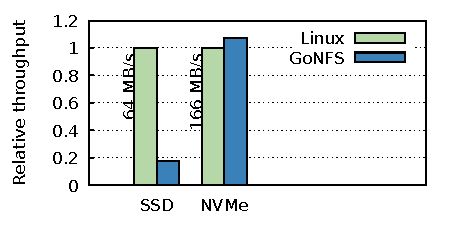
\includegraphics[scale=0.9]{fig/largefile-alt.pdf}
  \caption{Performance of \cc{largefile} depends on the storage medium. Linux
    takes advantage of unstable writes to write a large amount of data between
    barriers but \gnfs flushes to disk frequently.}
  %\caption{Performance of \cc{largefile} on a slow SSD across a few
  %  configurations. \tej{I wanted a cluster per configuration, and colors to
  %    correspond to the system.}}
\label{fig:largefile}
\end{figure}

% \begin{figure}[ht!]
%   \centering
%
%   \includegraphics[scale=0.9]{fig/aws/bench.pdf}
%
%   \caption{Performance of Linux NFS and \txn + \gnfs for \cc{smallfile},
%     \cc{largefile}, and \cc{app} workload, on a RAMdisk. \joe{This was run on an
%       AWS i3.metal with a Go in-memory disk.}}
% \label{fig:perf-aws}
% \end{figure}
%
% \begin{figure}[ht!]
%   \centering
%
%   \includegraphics[scale=0.9]{fig/aws/bench-ssd.pdf}
%
%   \caption{Performance of Linux NFS and \txn + \gnfs for \cc{smallfile},
%     \cc{largefile}, and \cc{app} workload, on a fast NVMe SSD. \joe{This was run
%       on an AWS i3.metal.}}
% \label{fig:perf-aws-ssd}
% \end{figure}

We first evaluate \gnfs's performance with a single client issuing requests.
\autoref{fig:perf} shows the results on the Intel Xeon desktop with both file systems backed by RAM, to
avoid any I/O overhead --- \gnfs takes a simple Go interface for the disk, which
we implemented with a large array, while ext4 uses a file in
tmpfs.\footnote{Running \gnfs on tmpfs performs slightly worse due to the around
  1 microsecond syscall overhead of each disk operation, which ext4
  does not incur since everything happens within the kernel.} \gnfs achieves at
least the throughput of ext4 across the different workloads.

On both the NVMe and slower SSD, \txn's performance relative to ext4 is similar on the \cc{smallfile} and \cc{app} workloads (not plotted),
again achieving at least 90\% of the throughout of ext4.
%
% next consider the effects of I/O overhead on disks. For the
% \cc{smallfile} and \cc{app} workloads, \txn's performance relative to ext4
% on both the NVMe and slower SSD is similar to ramdisk,
However, \gnfs performance on the \cc{largefile} benchmark is sensitive to disk I/O characteristics,
as shown in \autoref{fig:largefile}. On the faster NVMe device, \gnfs's large file performance
is comparable to ext4's, but on the slower SSD, it drops to under 20\% of ext4's throughput.
The reason is that the \cc{largefile}
benchmark produces a large number of parallel, unstable writes to the same file.
\gnfs runs them sequentially due to a per-inode lock, and then journals sequentially because it
ignores the unstable write flag. A disk barrier on the SSD takes about 2
milliseconds, so getting good disk throughput requires writing a large amount of
data before issuing a barrier, and the 64~KB batch size is insufficient to get
the maximum SSD write throughput. Re-running the experiment with
unstable writes enabled in \gnfs raises its throughput to 90\% of ext4's.

% The figure shows that \gnfs achieves
% comparable performance when using unstable writes, because even though the
% writes are issued sequentially \txn commits them to disk in large batches. Both
% systems get the same low performance if the benchmark is changed to consist of
% sequential, stable writes with the NFS client's \cc{sync} mount option, causing
% ext4's journaling behavior to match \gnfs in order to guarantee each write is
% persisted before the next is issued.

% shows the relative performance on this workload.

% \ralf{Are we switching to a different figure here?
% Namely Figure 19, which the comment says we will cut?}
% When run on a fast NVMe disk, relative
% performance is nearly identical. \tej{James suggested using the NVMe numbers as
% the main results and mentioning RAMdisk in passing.} \gnfs is able to achieve 90--95\% of the
% throughput of ext4 across the different workloads. We expect \gnfs and \txn to
% be somewhat slower, because they are written in Go rather than C, but \txn does
% implement sophisticated performance optimizations such as in-place updates of
% buffers, full-block overwrites without read-modify-write, etc. This suggests
% that \txn is a realistic journaling system for performant storage applications.
%
% On an SSD, \txn gets comparable performance for the \cc{smallfile} and \cc{app}
% benchmarks but is slower than Linux for the \cc{largefile} benchmark, as seen in
% \autoref{fig:perf-ssd} which shows relative throughput on the same benchmarks as
% \autoref{fig:perf} but on an SSD instead of a RAMdisk. We further explored the
% performance of this benchmark by running a number of other configurations, shown
% in \autoref{fig:largefile}. The \cc{largefile}
% benchmark produces a large number of parallel writes to the same file, which
% \gnfs runs sequentially due to a per-inode lock and journals sequentially due to
% the use of stable writes. The SSD can get 150 MB/s with sequential writes, but
% this requires writing a large amount of data before issuing a disk barrier,
% larger than the 64~KB write batch size. The figure shows that \gnfs achieves
% comparable performance when using unstable writes, because even though the
% writes are issued sequentially \txn commits them to disk in large batches. Both
% systems get the same low performance if the benchmark is changed to consist of
% sequential, stable writes with the NFS client's \cc{sync} mount option, causing
% ext4's journaling behavior to match \gnfs in order to guarantee each write is
% persisted before the next is issued.
% increasing the write batch size further to 128~KB also improves performance.

%\mfk{this paragraph doesn't have a clear narrative. it also seem to imply
%  that DFSQ has more CPU overhead because its implementation is more
%  sophisticated; i thought it was primarily due to Haskell}
%Compared with DFSCQ (a verified file system implemented by extracting Haskell
%code from Coq), \gnfs has equal or better performance, even with a single
%thread. We ran the same set of workloads to compare, and the only benchmark
%where DFSCQ has comparable performance is the in-memory \cc{smallfile} benchmark. For
%the other benchmarks and on an SSD, it obtains 40-60\% of the throughput (not
%plotted), even when DFSCQ is run through FUSE without the overhead of NFS. This
%is due to CPU overhead, since DFSCQ has a more sophisticated logging design than
%\gnfs that more aggressively buffers writes in memory. DFSCQ is single-threaded
%so with multiple concurrent clients throughput only gets worse.
%\tej{Do we want to put this in some plot, even if it's smaller? It's confusing
%to discuss results that aren't shown. Or, we may simplify our comparison to
%``it can be much worse and is never better''}

\subsection{\txn concurrency improves performance}
\label{sec:eval:concur}

To test whether the concurrency of \txn is important for performance we
measure the aggregate throughput of \gnfs with an increasing number of
clients that run the \cc{smallfile} benchmark.  We run the experiment
on a physical disk instead of an in-memory
file system so that while a thread is waiting for the disk another thread
can run.  We compare the performance of \gnfs to that of Linux ext4,
and to a single-threaded version of \gnfs that has no concurrency.

\autoref{fig:scale} shows the results on an EC2 i3.metal instance with an NVMe
SSD.  Both \gnfs and Linux ext4 take advantage of concurrent requests to
increase throughput.
The single-threaded \gnfs does just barely improve performance, from
parallelization among the clients and NFS server, but this amounts to less than
$2\times$ throughput with 20 clients than with one. Even with one client, \gnfs
achieves 35\% higher throughput than
single-threaded \gnfs due to concurrency between the RPC thread,
the logger thread, and the installer thread.  \gnfs achieves higher
throughput than Linux ext4, but it is hard to pin down the reason why,
because there are many differences in the designs.  One possibility
is that Linux ext4 does not have concurrent logging and installation
(but \txn does); another possibility is that ext4 waits for outstanding
transactions to finish before flushing to disk (but \txn does not).

\autoref{fig:scale-ssd} shows the scaling of \gnfs and Linux, this time on the Xeon desktop with a
slower SSD. While \gnfs obtains comparable performance for 7 or fewer cores,
Linux scales linearly beyond while \gnfs does not. The scaling in this case
primarily comes from batching writes from concurrent clients, resulting in
better disk write throughput.
\txn is not as careful about this, sometimes committing a small amount of data
rather than gathering many multi-writes and issuing them
together. The NVMe experiment in \autoref{fig:scale} uses storage with fast
enough random-write access that CPU efficiency is more important than issuing
large sequential writes; while a disk barrier takes 2 milliseconds on the SSD it
takes only 30 \emph{microseconds} on the NVMe disk.

\begin{figure}[ht!]
  \centering

  \includegraphics[scale=0.9]{fig/aws-spectre/scale.pdf}

  \caption{Combined throughput of multiple parallel \cc{smallfile}
    microbenchmarks, each creating files in different directories,
    on an NVMe SSD.}
  \label{fig:scale}
\end{figure}

\begin{figure}[ht!]
  \centering

  \includegraphics[scale=0.9]{fig/scale.pdf}

  \caption{Combined throughput of multiple parallel \cc{smallfile}
    microbenchmarks, each creating files in different directories,
    on a (slow) SSD.}
  \label{fig:scale-ssd}
\end{figure}

\subsection{Journaling atomicity simplifies proofs}
\label{sec:eval:atomic}

Many storage systems use journaling because they simplify the
implementation in terms of crash safety: the only point at which durable
state is modified is when an operation commits.  A goal of
\txn is to carry this insight into proofs, so that a storage system
using the journal can prove an operation is atomic using reasoning about durable
storage only at the commit point.

One measure of how well \txn achieves this goal is the lines of code in
\simplenfs that require reasoning about durable state.  \simplenfs
consists of \simplenfsLOC{} lines of verified code.  Only \simplenfsCrashLOC{} lines of code require
proofs to explicitly consider durable state, using crash conditions.
In \autoref{fig:write}, for example, crash reasoning is only needed for lines
6--8 when acquiring and releasing with the crash-aware lock specification.  All
of the other
code does not require reasoning about durable state; it suffices to prove
simple crash-free specifications that have a pre- and post-condition, but
no crash condition.  This formal reasoning is enabled by two techniques
from Perennial: lifting disk-object ownership and crash framing.

% \paragraph{Lifting disk-object ownership.}
% Lifting simplifies reasoning about disk-object ownership in \simplenfs in
% two ways.  First, lifting enables \simplenfs to transfer a predicate about
% disk-object ownership into a predicate about in-memory transaction state.
% Subsequent reads and writes within a transaction can operate on the
% transaction state, without worrying about durability until commit.
% Second, lifting enables \simplenfs to transfer predicates about
% disk-object ownership across crashes, to prove that on-disk state is
% correctly preserved on recovery.

% \paragraph{Framing the crash condition.}
% To formally prove that transactions are crash-safe, \simplenfs uses crash
% condition framing.  Specifically, when \simplenfs lifts some predicate
% into a transaction (e.g., a predicate describing the state of the inode),
% the proof immediately uses the durable disk-object ownership to frame
% away the crash-condition obligation until the commit point.  Using the
% durable resources to frame the crash obligation means that the durable
% resources are not available until commit, which in turn proves that they
% are not modified.  At commit time, the resources become available again,
% and the developer must explicitly reason about their crash safety (e.g.,
% just in the code shown in \autoref{fig:writecommit}).


\subsection{Perennial enables modular crash reasoning}
\label{sec:eval:modular}

Atomic crash specifications are crucial for enabling modular reasoning
about crash safety.  In \txn, atomic crash specs are used at many
layer boundaries.  Out of the layers shown in \autoref{fig:layers},
\textsc{circular}, \textsc{wal}, \textsc{obj}, and \textsc{jrnl} all
provide atomic crash specifications, which are used by the layer above. One benefit of atomic crash specs is that they
allowed us to develop these layers independently, using the specifications of
lower layers before their implements were fully proven, as one would
expect of any good API.

The modularity in Perennial largely follows the same structure as the code.
\autoref{fig:loc} shows that the \textsc{wal} and \textsc{jrnl} proofs were
split into an atomic transition specification about the code and a proof-only
abstraction on top, but the bulk of the division was due to boundaries in the
code that made the implementation manageable. Using separation logic it was easy
to prove data structures (like the striped lockmap) and individual utility
functions and use their abstract specifications elsewhere in the proof.

\subsection{Proof effort}
\label{sec:eval:proof}

\autoref{fig:loc} shows the lines of code and lines of proof for \txn
and \simplenfs.  The hardest part of \txn lies in the \textsc{wal}
layer, which has significant lock-free concurrency, and requires careful
reasoning about crashes and recovery.  This is reflected in \textsc{wal}'s
relatively high lines of code, lines of proof, and proof:code ratio.
In contrast,
\simplenfs leverages GoJournal's atomicity, and ends up with a
much smaller proof relative to its code size.


\subsection{Verification prevents bugs}
\label{sec:eval:bugs}

% When developing \simplenfs and
% \txn, we wrote extensive unit tests, but they were not sufficient to
% find all bugs before proving.  When proving \simplenfs, we discovered
% several bugs due to uncaught integer overflows (which wrap around in Go) and
% out-of-bounds reads and writes that could have led to file-system corruption
% (e.g., if the write RPC includes an offset and count that, if added together in
% 64-bit arithmetic, overflows to a value less than the current size of
% the file).

When developing \txn, we wrote unit tests to quickly find problems before starting
verification, but they did not catch all bugs. While proving
\txn, we found a subtle bug in absorption.  When appending a new
transaction in memory, \txn has an optimization called absorption where earlier
writes to the same address are replaced with the new values. However, we discovered a race condition,
where the logger thread could have been already flushing those earlier
writes to disk, leading to unpredictable disk contents depending on the
order of absorption vs logging.  We fixed this issue by introducing the
\cc{nextDiskEnd} boundary, as shown in \autoref{fig:log}: the logger thread only
logs up to \cc{nextDiskEnd}, and absorption is only allowed to modify values
after \cc{nextDiskEnd}.


% Caught a bug where a variable got changed and then we read the new value: \url{https://github.com/mit-pdos/goose-nfsd/commit/255a1c4cc}.
% Forgot to check for out-of-bounds: \url{https://github.com/mit-pdos/goose-nfsd/commit/5cb7b82b9c809}
% Couple missing overflow checks: \url{https://github.com/mit-pdos/goose-nfsd/commit/f5d41e3926c2}, \url{https://github.com/mit-pdos/goose-nfsd/commit/31cc9dcc1}
% Check for inode read past end: \url{https://github.com/mit-pdos/goose-nfsd/commit/b91113936d27}
% added an optimization to make the proof easier: \url{https://github.com/mit-pdos/goose-nfsd/commit/a788305ba0d7}
% introduced data structure (sliding) for mem log to make verification more modular
% introduced layer for on-disk circular log to make verification more modular

% \mfk{describe trusted computing base somewhere: here or in system overview?}

\section{Conclusion}
\label{sec:concl}

\txn is the first concurrent crash-safe journaling
system with a machine-checked proof, built on top of the Perennial 2.0 framework.
\txn uses Perennial's techniques, including lifting and crash framing, to
carry over the atomic benefits of journaling to its formal specification.
This enables storage applications to use mostly crash-free reasoning in
their proofs.  For example, in the verified \simplenfs server, only \simplenfsCrashLOC{}
lines of code, out of \simplenfsLOC{}, required crash reasoning.  \txn is sophisticated
enough to implement a functional (but unverified) NFSv3 server, \gnfs, that achieves
90\% of the performance of a Linux ext4 NFSv3 server on a development workload, far higher than
any previous verified file systems, and \txn's concurrency enables \gnfs
to scale with concurrent client requests.  To simplify \txn's proofs,
Perennial provides logically atomic crash specifications, which capture the
crash properties of internal interfaces as single logical transitions,
enabling modular proofs for \txn's internal layers.



\chapter{Conclusion}%
\label{sec:conclusion}
This thesis describes an approach to verify software with a combination of
concurrency in the implementation and crash-safety guarantees, applied to the
DaisyNFS file system. It spans from foundations for verifying this software in
general through the design and proof of the file system itself. The foundations
include Perennial, a program logic for crashes and concurrency, and Goose, an
approach for reasoning about Go code. DaisyNFS is designed around a verified
transaction system called GoTxn, which makes it feasible to scale verification
by enabling sequential reasoning for transactions on top.

\section{What is the value of verification?}

The reader might wonder about the broader value of verification and the
contribution of the thesis. This section makes some broader points about the
value of verification, both in general and in the specific case of this thesis.

\paragraph{Verification is valuable for critical systems.} It will never be cost
effective to verify all software; at a minimum, for verification to be useful a
piece of software needs a specification that is more likely to be correct than
the implementation.
Instead, the aim is to use verification for critical systems, \emph{critical}
because failures are especially bad, and \emph{systems} that have well-defined
guarantees to make to other systems and applications running on top. It is also
helpful in the cost-benefit tradeoff if the system is part of a ``narrow waist''
used by many other pieces of software, since then the impact of bugs is felt to
a greater extent. Finally, alongside the need for a specification it is also
important that the verification respond to changes in both specification and
implementation. If both change rapidly and the proofs cannot be re-done, then
verification won't keep up with the pace of development. File systems fit all of
these criteria: bugs can lead to data loss which the application cannot
mitigate, the interface is stable and relatively standard, and essentially all
applications go through the file system to store persistent state.

\paragraph{Cost versus benefit.}
I think about verification in terms of whether the benefits in terms of
reliability outweigh the costs of writing the proofs. Research in verification
generally aims to reduce the cost, or to identify areas with particularly large
benefits. This thesis in particular focuses on making verification of crash-safe
and concurrent systems possible, in order to give an upper bound on the cost.
Further research would hopefully bring the costs down so that verification is an
appealing approach for the next generation of storage systems.

A real achievement for verification would be to use verification not just as
alternative to the practices above, but to build something with more daring optimizations,
features, or speed than would otherwise be possible; this would increase the
benefits rather than decreasing the cost. Storage systems that holds persistent
state have the potential to be just such an application. There aren't that many
widely-used
file systems --- most people use one of ext4, btrfs, or XFS on Linux, NTFS on
Windows, and APFS on macOS --- and new file systems are generally adopted
slowly. APFS was surprising for having only a 3-year development period before
Apple widely deployed it. Ext4 is the next newest of that list, introduced in
2008 (by extending ext3, which was first released in 2001). Verification has the
potential to create a file system that is more rapidly adopted by virtue of its
proof. This might be especially applicable for some new hardware, like a file
system for persistent memory or new zoned storage (ZNS) SSDs.

% ext4: 2008
% ext3: 2001
% XFS: 1994 (first released on IRIX OS for SGI)
% NTFS: 1993
% APFS: 2017

\paragraph{Mechanized proofs can be adapted to change.} Informal
reasoning even with a program logic can gain much of the value of formal
reasoning in that it helps the author think systematically, and permits varying
the level of detail to suit the author's needs. However, a complete and
mechanized proof is especially valuable when it comes to \emph{changing} the
code and proof: it is difficult and tedious to make a systematic change to an
on-paper proof and be confident that all relevant parts of the proof have been
re-analyzed and updated.

In contrast, a mechanized proof can be updated and re-checked, particularly in
an automated tool. In developing the DaisyNFS Dafny proof, I had a wonderful
experience with adapting a proof when adding indirect blocks: at some point a
function verified before I had even understood if or why it was correct!
Adapting existing proofs in an interactive theorem prover is more challenging
than with automated tools (although there is a relatively new field of \emph{proof
repair}~\cite{ringer:proof-repair} that aims to address this), and we found
adapting the GoTxn proofs in Perennial to be more challenging.
\Cref{sec:eval:incremental} talks about incremental changes in the work
described by this thesis in particular.

\paragraph{Verification helps discover accurate, precise specifications.} Some
systems are extremely reliable, due to extensive testing, real-world usage, and
development, but they still lack a clear description of the interface exposed.
The process of verification helps discover a precise, mathematical
specification, and the proofs confirm that this specification is actually an
accurate description of the implementation. Precise and accurate specifications
are useful even for unverified software. While documentation is a helpful form
of informal specification, mathematical specifications have the advantage of
reducing ambiguity.

One example from the work in this thesis came up in the GoTxn write-ahead log
specification. When we came up with the idea of a history of multiwrites as the
specification, we able to explain absorption, where a value overwrites an older
write that hasn't been logged yet, as an optimization and not a detail the
caller should be concerned with. Merely writing down the specification also
helped clarify some of the internal invariants. Another example was some
difficulty we ran into interpreting the description of ``weak-cache consistency
(WCC)'' metadata in the NFS protocol. The RFC explains this aspect in several
places and combines describing what information should be returned, rationalizes
the need for this feature, and describes how the client should use it. A
mathematical description teases these apart so that the first is formally
described and the rest are commentary on top. The end result was quite simple:
the server should return both the old attributes and final attributes of
whatever file or directory the WCC data pertains to. Because these attributes
include modification timestamps, they permit the client to invalidate their
local cache when the old timestamp doesn't match the client's cached value.

\paragraph{Verification guides debugging.} With a verified system, bugs are
still inevitable since there is unverified code surrounding the verified code,
the assumptions of the proof can be violated, and the specification can be
wrong. However, an advantage of formal verification, particularly fully
machine-checked proofs, is that when bugs are discovered it's safe to start
debugging with all the code outside the verification as well as looking at the
specification. We ran into several bugs while developing DaisyNFS; several are
described in \cref{sec:eval:testing}. Some were due
to incorrect specifications; for example, at one point we returned the wrong
``before'' WCC data, causing Linux to constantly invalidate its cache and send
extra RPCs and reducing performance. Others were due to unverified code
violating the assumptions in the verified code.

% \paragraph{Interactive theorem proving is a great way to prototype.} I do not
% anticipate that busy engineers trying to write production code will write proofs
% in Coq, much less develop a custom program logic. However, this workflow is
% excellent for prototyping the right reasoning principles, some reasons for which
% are outlined above. Working out proofs interactively gives a good feel for how
% the logic works, from which automation can be designed bit by bit (some of it as
% Coq automation itself). In Perennial (as in Iris), proof steps are at a
% sufficiently high level of abstraction to make the proofs doable for prototyping
% purpose, even though it has no search-based automation, sophisticated
% algorithms, or use of an SMT solver.


\paragraph{Mechanized proofs help develop a sound logic.} Within verification
there is a spectrum of formality that includes ``foundational'' techniques like
Perennial with a soundness theorem as well as tools like Dafny that generate
verification conditions for a solver but no proof of soundness. When developing
a new program logic, one reason to go through the trouble of mechanizing the
proofs and carrying out a soundness proof is to validate the program logic
itself. For example, the formalism helps work out a specification for crash
safety and concurrency, one that the mechanized proof shows has the right
meaning (due to the soundness theorem) and is usable (due to the verified
reasoning principles in the logic). After gaining confidence and intuition with
the safety-net of a soundness proof, it is possible to make further progress
with informal reasoning, or by implementing the logic in an automated system.

Concurrency makes soundness especially challenging and important, since specifications can be quite
subtle to use. One recent example is prophecy variables, where in the process of
developing a mechanized proofs Jung et al.\ found an unsoundness in the use of
prophecy variables in a proof from Viktor Vafeiadis's PhD
thesis~\cite{jung:prophecy,vafeiadis-phd}, a proof that was conducted informally
and on-paper. Higher-order reasoning, especially the ability to store procedures
in the heap, has also led to some subtle reasoning principles like the
anti-frame rule~\cite{pottier:anti-frame}, whose soundness proof was rather
sophisticated~\cite{schwinghammer:semantic-anti-frame}.


\section{Discussion}

\paragraph{Memory safety at interface boundaries.}
A surprisingly difficult aspect of the proof was addressing memory safety
considerations while describing interfaces.
DaisyNFS has two important interface boundaries, one between GooseLang and the
disk, and another to describe the GoTxn interface. Both APIs involve data in the
form of byte slices. The challenging aspect of using bytes in a method is
specifying how \emph{ownership} transfers. For example, the \cc{DiskWrite(a, v)}
operation passes a buffer \cc{v} to the disk. It could be that ownership of
\cc{v} needs to be transferred to the disk, since it uses the buffer later, or
that \cc{v} should be read-only for the duration of the call and ownership is
returned to the caller, or that if \cc{v} is permanently read-only the disk and
caller can share the buffer.

Expressing ownership as a logical idea in the logic is relatively easy using
separation logic, but the semantics of \cc{DiskWrite(a, v)} has to be
axiomatized since it is part of an external interface. In order to simplify expressing the ownership transfer, the
GooseLang \cc{DiskRead} returns a freshly allocated buffer, but it would have
been better for performance if the caller supplied a buffer that the
\cc{DiskRead} wrote to (as in the usual \cc{read} system call). Similarly, the
GoTxn interface to Dafny makes additional copies to simplify ownership
reasoning, especially in the transaction refinement proof. A better solution would
have been to develop a specification style for expressing ownership in the
semantics of the operations themselves, along with associated reasoning
principles.

Rust would assist with better handling of ownership in interfaces, but does
not completely solve the problem. Where it would fit in is that if an interface
makes \emph{assumptions} about ownership transfer, Rust would help in enforcing
those assumptions at compile time. While convenient for the verified code to
know if ownership is violated before attempting a proof, this would be
especially good for enforcing that code calling into a verified interface
respects its assumptions about ownership. What Rust doesn't solve is that it is
still necessary to express ownership assumptions in the interface, a challenge
independent of the implementation language.

\paragraph{Read-only sharing.}
Another challenge, related to memory safety, was reasoning about read-only
sharing in the internals of GoTxn. Changing data structures after they were written to support read-only
sharing was difficult, since every specification needs to incorporate fractional
permissions. Read-only locking was challenging to retrofit support for, even
though it may have improved read-read concurrency in GoTxn and DaisyNFS. This
also showed up in the data structure for the in-memory log, which needs to share
read-only data blocks between threads issuing reads to the write-ahead log, the logger
thread, and the installer thread.

\paragraph{Modular proofs.}
\Cref{ch:crash-logatom} describes a style for specifying a library in Perennial.
Modularity was essential to enable the GoTxn proof. Better support for
modularity, perhaps formalizing some of the aspects of the specification style,
would have more cleanly separated each library's proofs. Where this is
particularly important is in making changes to the code that affect an
interface, in which case it can be difficult to tell from the code exactly what
properties the caller is assuming about the interface. The specification style
was developed in parallel with all the proofs, which means that proofs do not
all follow the best practices developed along the way.

\section{Future work}

\paragraph{Apply the approach to Rust or C.} It would be interesting to port
the Goose approach to Rust or C. This would not necessarily be for better
performance but as a first step towards better systems integration. For example,
Rust or C would be more practical for verifying critical parts of the Linux
kernel. An important challenge for verifying in-kernel code would be modeling
the specifications, both those assumed by the verified code and what is promised
to the rest of the kernel.

\paragraph{Asynchronous model of the disk.} The disk model in Goose assumes
writes are durable as soon as the write returns, but real disks typically buffer
writes internally. Goose has a new asynchronous disk model, used for an
independent example, but it would be good future work to change GoTxn to use
this new model. Above the write-ahead log this should have no effect on the
specifications. Going beyond asynchronous durability, it would also be
interesting to model a different interface entirely like that of libaio where
requests are submitted to a queue and completions are delivered separately.

\paragraph{Improve the write-ahead log.} After implementing GoTxn, we made
relatively few changes, as reported in \cref{sec:eval:incremental}. Several
improvements to the write-ahead log would be interesting to make, which were
challenging due to the complexity of the existing proof.

First, it would be worth experimenting to see if the proof of installation could
be separated from the rest of the proof. The important task would be identifying
the right specification for the logging code which is enough to reason about the
combination of installation and logging.

Second, due to the future dependency in the write-ahead log's \cc{Read}
(described in \cref{sec:txn:wal}), it is specified as two separate
operations; it would be interesting to add \emph{prophecy variables} to
Perennial, similar to the Iris implementation~\cite{jung:prophecy}, and give
\cc{Read} a single linearizable specification.

Finally, the write-ahead log uses physical logging where all updates represent
full-block overwrites. It would be interesting to add more sophisticated
operations like sub-block updates that are natively supported by the write-ahead
log (rather than by the layer above). More ambitiously, it would be interesting
to verify \emph{logical logging} where updates represent high-level operations
like a file write. Logical logging would require a more sophisticated
specification and proof because the write-ahead log's entries would be
interpreted by the caller, resulting in a higher-order specification where the
caller passes a function which might need to be run during recovery, and
multiple times.

\paragraph{Verifying a file system directly on top of GoJournal.} Dafny allows
the DaisyNFS proof to take advantage of automation that is enabled by sequential
reasoning. It would be interesting to do a direct comparison against a proof in
Perennial where due to ownership the proofs would still require only sequential
reasoning. The GoJournal paper reports verifying a subset of a file system
directly~\cite{chajed:gojournal}, but we never attempted to apply the approach
to a full-fledged file system. What would be especially interesting is if the
Perennial proof started with the Dafny proof's structure and invariants; perhaps
these invariants (developed under the constraints of Dafny and for
automation-friendliness) would also be useful in an interactive theorem proving
setting.

\paragraph{Do more with the NFS specification.} The NFS specification for
DaisyNFS is hand-written and integrated with the code. It would be an
interesting project in its own right to turn this into a complete, well-tested
formalization of the RFC. For example, the Dafny specification could make a serious
attempt to capture all the non-determinism allowed by the RFC. As a standalone
artifact the specification could also be used to test servers (comparing to the
allowed behaviors). An executable version of the specification (though perhaps
inefficient and not durable) would be valuable to test the specification itself
and explore what clients do when faced with different server behavior.


\backmatter

% single spacing for bibliography
\begin{spacing}{1}
\bibliography{n-str,paper,n,n-conf}{}
\bibliographystyle{abbrvnat}
\end{spacing}

\end{document}
